\section{Choice of methods}
\lb{sec:methods}

\subsection{General methodology}
We will use data-driven approach in constructing the probabilistic catalog.
The result depends on two inputs: data used for constructing the model and the choice of the method for classification.
The data in our case will be sources in 3FGL with known classes. 
We will split the data into training and testing subsets.
For the methods, we will consider four machine learning algorithms: boosted decision trees (BDTs),  random forests (RF),
logistic regression (LG), and neural networks (NN).
The resulting probabilities of classification depend on the choice of the classification algorithm.
Although some algorithms have slightly better performance on the test sample then others,
the overall performances are relatively similar.
As a result, we will report the classification probabilities for all four algorithms in the catalog, instead of selecting the 
``best'' one.
The difference among the predictions will serve as a measure of modeling uncertainty related to the choice of the classification algorithm.

\subsection{Discussion of the choice of the classification algorithms}
{\it Decision trees}
One of the most simple and transparent algorithms for classification is decision trees.
In this algorithm, at each step the sample is split into two subsets using one of the input features.
The choice of the feature and the separating value are determined by minimizing an objective function, such as misclassification
error, Gini index, or cross-entropy.
This method is very intuitive, since at each step the results can be described in words, 
for example, at the first step, the sources can be split in "mostly" Galactic and extragalactic by a cut on the Galactic latitude.
At the next step, the high latitude sources can be further subsplit into millisecond pulsars and other sources, buy a cut on the spectral index around 1 GeV (pulsars have a hard spectrum below a few GeV) etc.
One problem with decision trees is overfitting: if the tree is too deep, then it will pick up particular cases of the training sample, while too shallow tree would not be able to describe the data well. As a result, one needs to be very careful in selecting the depth of the tree.
This problem can be avoided if a random subset of features is used to find a division at each node. This is the basis of the RF algorithm,
where the final classification is given by an average of several trees with random subsets of features used at each node.
Another problem with the simple trees is that it can miss the classification of some subsets of data. In BDT algorithms, the final classification is given by a collection of trees, where each new tree is created by increasing the weights of misclassified samples of the previous step. 
Finally, simple trees predict classes for the data samples, while we would like to have probabilities of classes (also known as soft classification).
RF and BDT algorithms, by virtue of averaging, provided probabilities. As a result, we will use RF and BDT algorithms rather than simple trees in this paper.

Tree-based algorithms, even after averaging in RF and BDT methods, have sharp edges among domains with different probabilities.
In LR algorithm, the probabilities of classes are by construction smooth functions of features.
In particular, for two-class classification the probability of class 0, given the set of features $x$, is modeled by sigmoid (logit) function
\be
\lb{eq:logit}
p_0(x) = \frac{1}{1 + e^{m(x)}}.
\ee
The probability of class 1 is then modeled as $1 - p_0(x)$.
If $m(x)$ is a linear function of features, then the boundary between the domains, defined, e.g., as $p_0(x) = 0.5$, will be linear.
More complicated boundaries can be modeled by taking non-linear functions $m(x)$.
Unknown parameters of the function $m(x)$ are determined by maximizing the log likelihood of the model given the known classes of the data in training sample.
A nice feature of the LR method is that it, by construction, provides probabilities of classes with smooth transitions among domains of different classes.
A limitation is that the form of the probability function is limited by the sigmoid function in Equation (\ref{eq:logit}).

We notice that if $m(x)$ is a linear function of features $x$, then the logistic regression model is obtained by an application of sigmoid function to a linear combination of input features.
This is in fact a single layer perceptron, or a neural network, with several input nodes (each node corresponds to a features), one node in the hidden layer, and one output node, which corresponds to $p_0(x)$.
The output value is obtained by a non-linear transformation (sigmoid) of a linear combination of features.
Neural network with several hidden layers is obtained by a sequence of nonlinear transformations of linear combinations of features.
In particular, the values in the first hidden layer are obtained by a non-linear transformation of linear combinations of input features.
Then the values in second hidden layer are obtained by a non-linear transformation of  linear combinations of values in the first hidden layer etc.
In the context of neural networks, the non-linear transformations are called activation functions.
If the activation function for the output layer is sigmoid, then the output value (values) can be interpreted as probabilities.
We notice that in this case the neural network is can be expressed by a logistic regression for some function $m(x)$,
i.e., the neural network is then a particular way of constructing $m(x)$.
Thus the only difference between LR and NN for the classification problems is the construction of the function $m(x)$.
In this paper, for LR $m(x)$ will be constructed as a combination of low-order polynomials of the input features,
while for NN, $m(x)$ will be constructed by taking linear input features and several hidden layers, e.g., 4 or 5, 
in a fully connected neural network.

\section{Construction of a probabilistic catalog}

As an example of the construction of a probabilistic catalog, we will use with the 3FGL catalog.
For training and testing the methods, we use sources which have associations and no missing values in the catalog table.
In this paper we will perform a two-class classification to separate PS into pulsars and AGNs.
Thus, we subselect the sources, which are associated to either a pulsar or an AGN.
After the training of the algorithms, we test the performance with the test sources and predict the classes of sources without associations,
but have all features present in the catalog table.
The general workflow will have the following steps:
\ben
\item
Select data for learning and testing.
\item
Train algorithms using the learning dataset.
Tune hyper-parameters of the algorithms and test the performance on the test dataset, in particular, to avoid overfitting.
\item
Make prediction for unassociated point sources of the 3FGL.
We also apply the classification for associated source. In this case we check if there are any outliers among the associated sources.
\een
As a result of the analysis in this section, we obtain a catalog with probabilistic associations of sources in 3FGL.
We will report the classification probabilities for all four algorithms and each source.
In the next section we compare the predictions in the catalog with the new 4FGL catalog.
We also construct a probabilistic catalog starting with the 4FGL.


\subsection{Data and feature selection}

We restrict attention to associated and unassociated source but without missing values. 
We use the associated sources which were classified as either AGNs (classification labels in 3FGL catalog: agn, FSRQ, fsrq, BLL, bll, BCU, bcu, RDG, rdg, NLSY1, nlsy1, ssrq, and sey) or Pulsars (classification labels in 3FGL: PSR, psr), which results in a list of 1905 sources. 
%The rest of the sources without problematic values were then used as unassociated sources, which we used later on for testing and prediction. \\
%Our methodology for classification was dependent on two things: The data that we had, which needed to be cleaned and the algorithms that we needed to apply. For this we decided on using the 3rd catalog of F-LAT (3FGL from hereon) for initial training and testing, the 4th catalog (FL8Y from hereon) for further testing and predictions.
%Our data was similar to that used by Parkinson et. al. We cleaned the 3FGL catalog to have sources which were both associated and unassociated but with no missing values.\\

There are several tens of features of point sources quoted in the catalog, such as the position, photon and energy fluxes integrated in different energy bands, spectral parameters, variability index as well as corresponding uncertainties.
In our example, we use the following ten features:
flux density and the error on it, spectral index, spectral curvature, four hardness ratios (as defined in \cite{2016ApJ...820....8S}), variability, and the galactic latitude. 
We used the logarithmic scale for features with large spread of values, e.g., for the flux density, the error on flux, the curvature, and the variability. 
\begin{comment}
%The complete list of sources, along with some statistics, is given in the appendix. 
The influence of the features on the classification, especially the differences in the various methodologies is discussed in more details in the next section.
Not all of these parameters are independent, for example, log of the ratio of fluxes is proportional to the spectral index (if the spectrum is represented well by a power law) etc.
If two variables are highly correlated, then one can discard one of them, since the corresponding information can be recovered from the other one, the corresponding correlation matrix is shown in Figure \ref{fig:corr}.
In the following we will see that not all features are important for classification and further restrict our attention to the four features, which have the largest separating power for tree-based algorithms.

\end{comment}  
The feature statistics can be seen in the appendix.




\subsection{Construction of classification algorithms}

The number of tunable parameters in the classification algorithms are not fixed a priori. 
Moreover there is a certain freedom in the choice of the architecture of the algorithms, such as
the number of hidden layers and the number of neurons in the hidden layers in neural networks.
In general one starts with a simple model and increases the complexity (the number of tunable parameters)
until the model can describe the data well, but does not overfit it.
The overfitting is avoided by splitting the training data into the training sample, which is used for tuning the parameters,
and test sample, used to check that the model is not overtrained (for overtrained models the accuracy on the test
sample is significantly worse than the performance on the training sample).
We will split the data into 70\% training and 30\% testing samples.

The construction of the algorithms will proceed in two steps:
\bi
\item
Choose the number of free parameters in the model and tune them, so that the model fits the training data.
\item
Test the model in the testing sample.
\ei
The details of this procedure are given in the subsections below.

\begin{comment}
%In this section we provide details on the training of the ML algorithms for the classification of the PS.
We will split the sources with known classifications into training (70\%) and test samples (30\%).
One of the main objectives is to increase the accuracy of classification: this is achieved by adding more parameters to the model
and tuning them using the training sample.
The test sample is used to ensure that the algorithms do not overfit the data.


One of the main aims of our project was to understand and optimize the machine learning methods which we were using. So apart from the features which were in the data itself, we also theorized and experimented with the parameters of the algorithms themselves. We wanted to find the fastest and cost-effective way of using certain methods, without going into regimes of under and over-fitting the data. Parameters which we studied range from Depth and Number of trees in Forest based methods to the number of hidden layers and epochs in neural networks. The details are given in the next section, where we discuss our expectations and the resulting behaviour of our algorithms.\\


 All of the machine learning algorithms were taken from the python module sklearn, including Neural Networks. A neural network using Keras was also attempted; however, due to the classification being on only two classes, we discarded it in favour of the sklearn algorithm which was much faster.\\
One of the main aims of our project was to understand and optimize the machine learning methods which we were using. So apart from the features which were in the data itself, we also theorized and experimented with the parameters of the algorithms themselves. We wanted to find the fastest and cost-effective way of using certain methods, without going into regimes of under and over-fitting the data. Parameters which we studied range from Depth and Number of trees in Forest based methods to the number of hidden layers and epochs in neural networks. The details are given in the next section, where we discuss our expectations and the resulting behaviour of our algorithms.\\	

\subsection{Details of the analysis}

\subsection{Data and Features}

The total number of sources, including unassociated and associated, in the two catalogs is shown below. \\
\begin{figure}[h]
%\centering
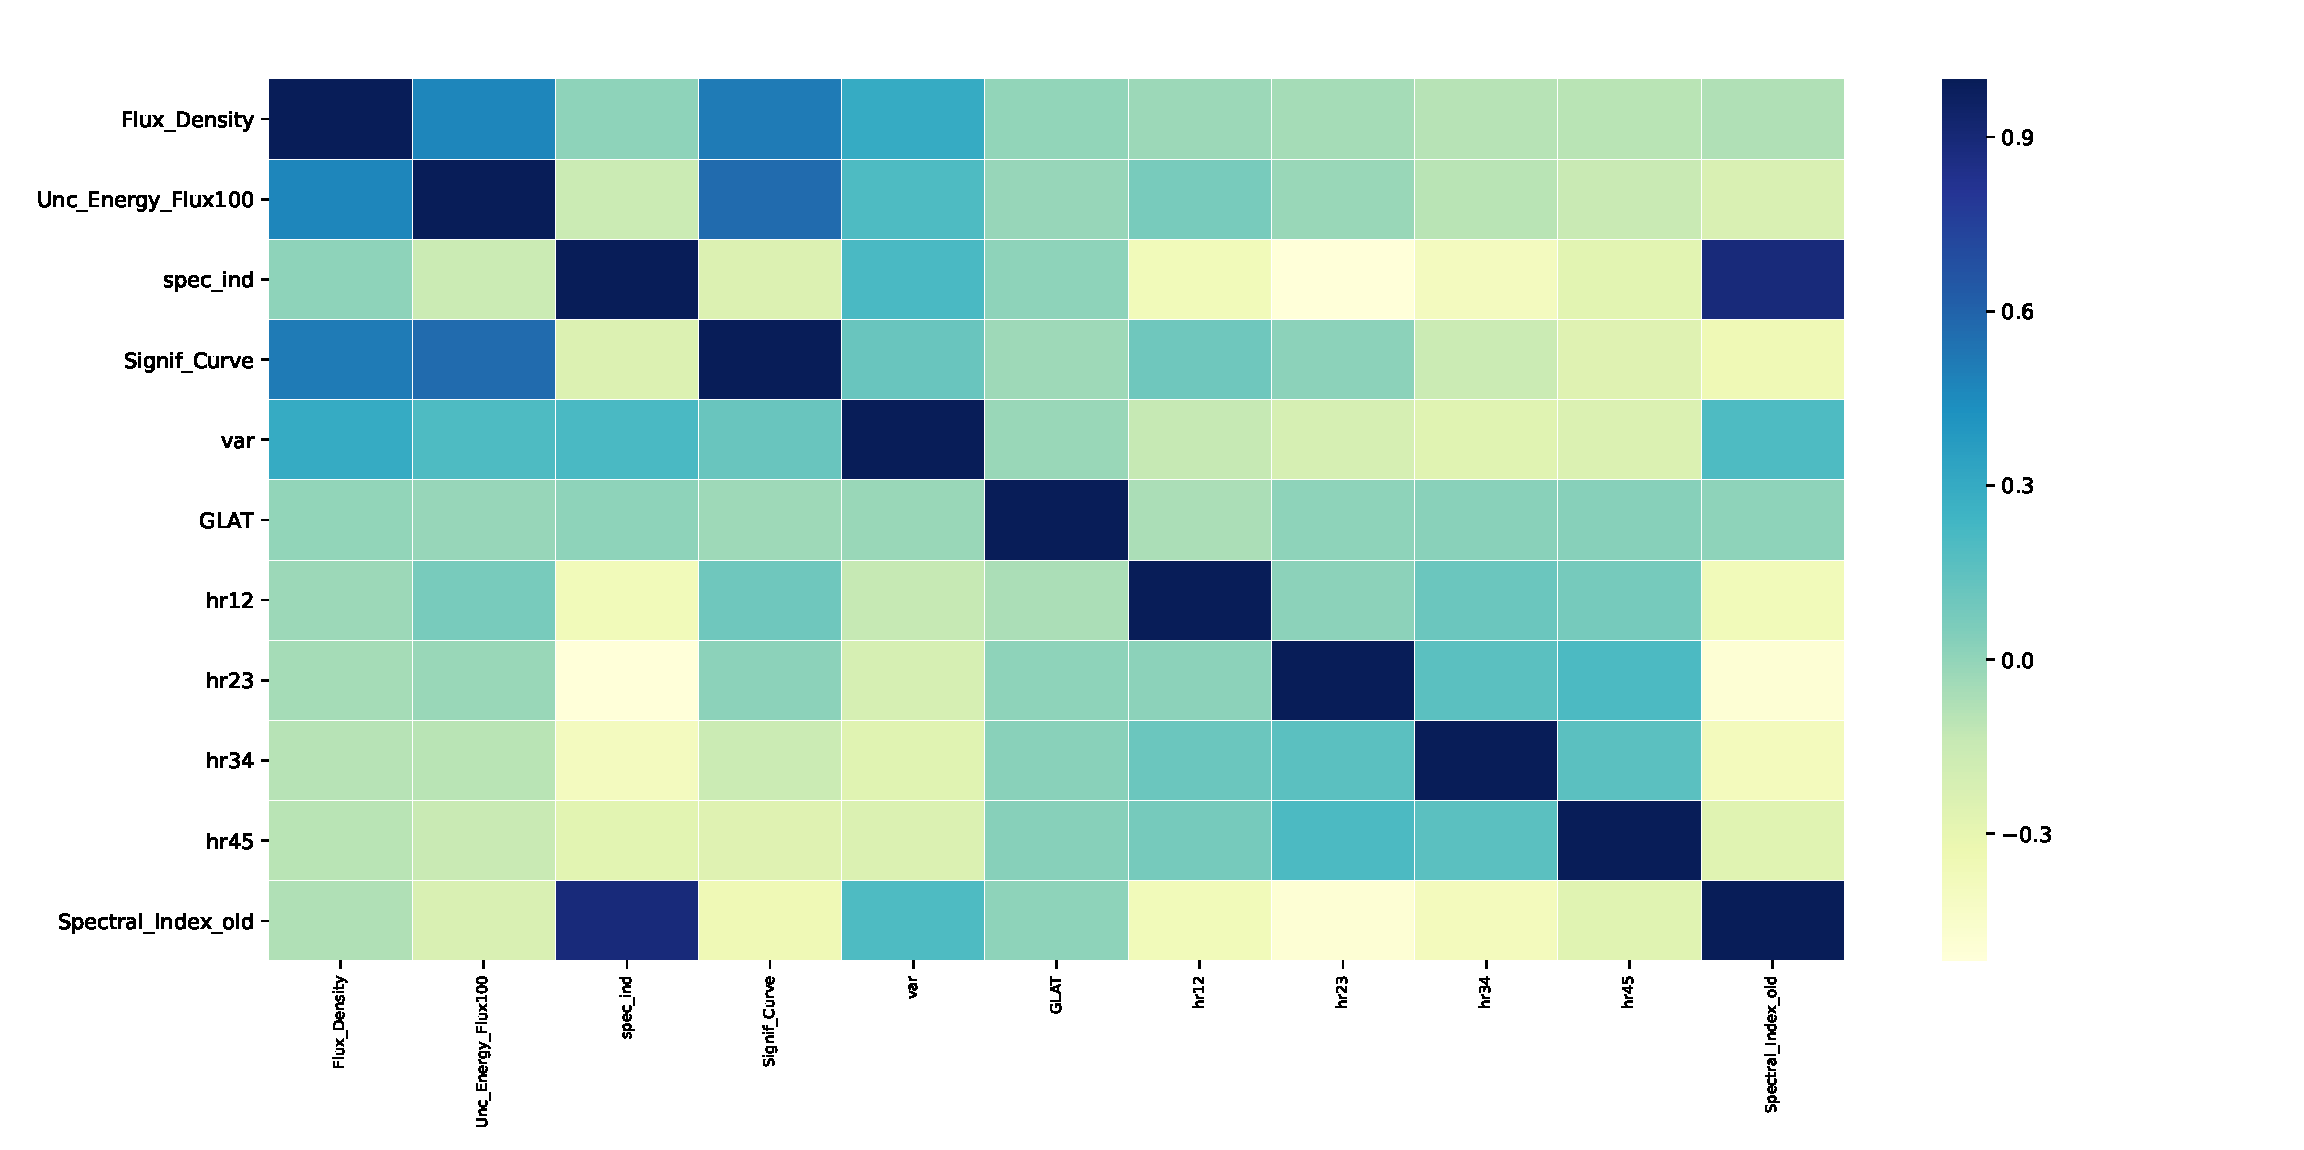
\includegraphics[width=\onepic\textwidth]{plots/correlation.pdf}
\caption{Correlation matrix for the most important features}
\label{fig:corr}
\end{figure}
[Add Table]\\

The features used for our analysis follow the same idea as the previous studies. The features, along with statistical and methodological details, are given below. A correlation matrix is presented for the most important features as well. The matrix is important for the case where there might be redundant features, in which case using only one of the two features would be a better idea.\\




Our initial hypothesis was that certain features would be more important for classification than others. For instance, as shown below, one can see a clear distinction between the regimes of AGNs and Pulsars, based on spectral idex and significant curvature. [Add image] While not clearly obvious from the get go, we were also interested in comparing the importance of features based on the algorithms that we were using. Due to the difference in the basic method of Random Forests and Neural Networks, we expected a slight shift in their reliance on certain features. Despite that we hypothesized that features with the most contribution would be among spectral index, variability, and the curvature; as already observed by Parkinson et. al. This is made clearer by the two figures below, which highlight the separation of PSR and AGN. The separation is seen to be much easier when spectral index and curvature are used, as opposed to the flux and uncertainty on the flux.\\

\begin{figure}[h]
%\centering
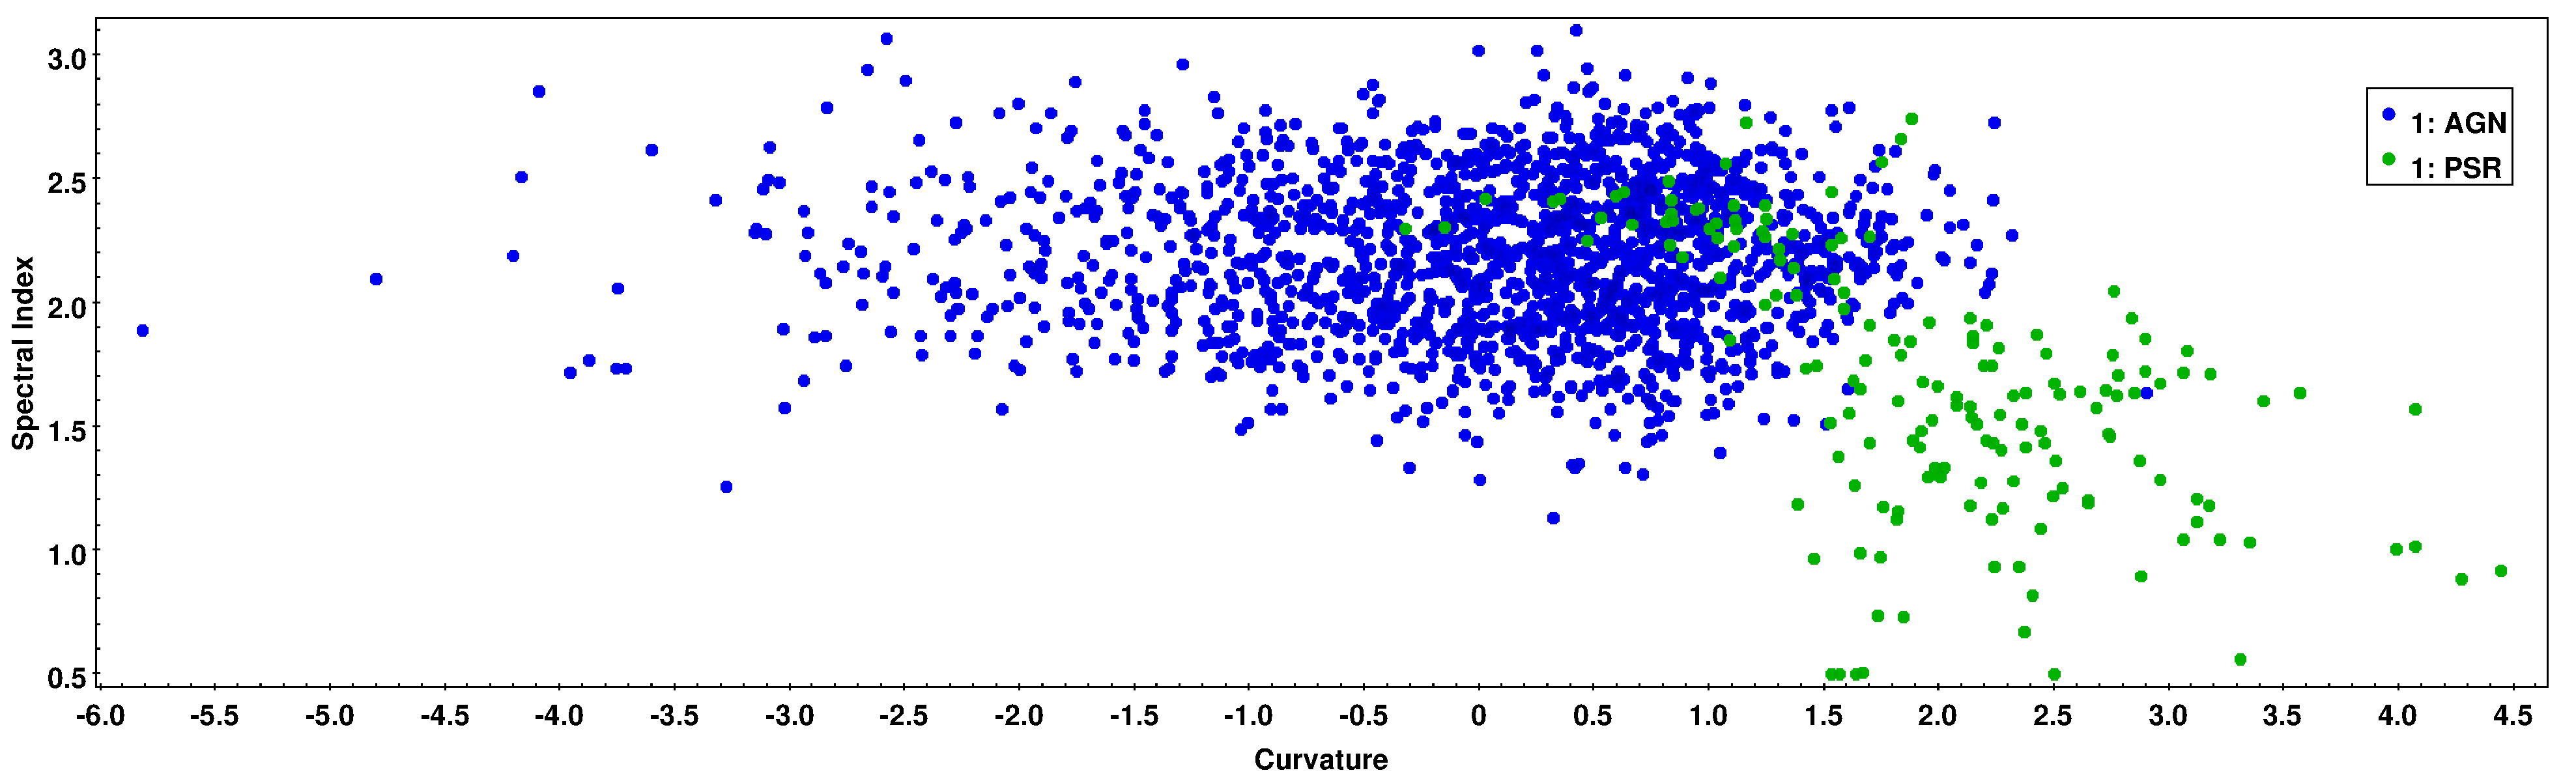
\includegraphics[width=\onepic\textwidth]{plots/signifcurvvsspecind2.pdf}
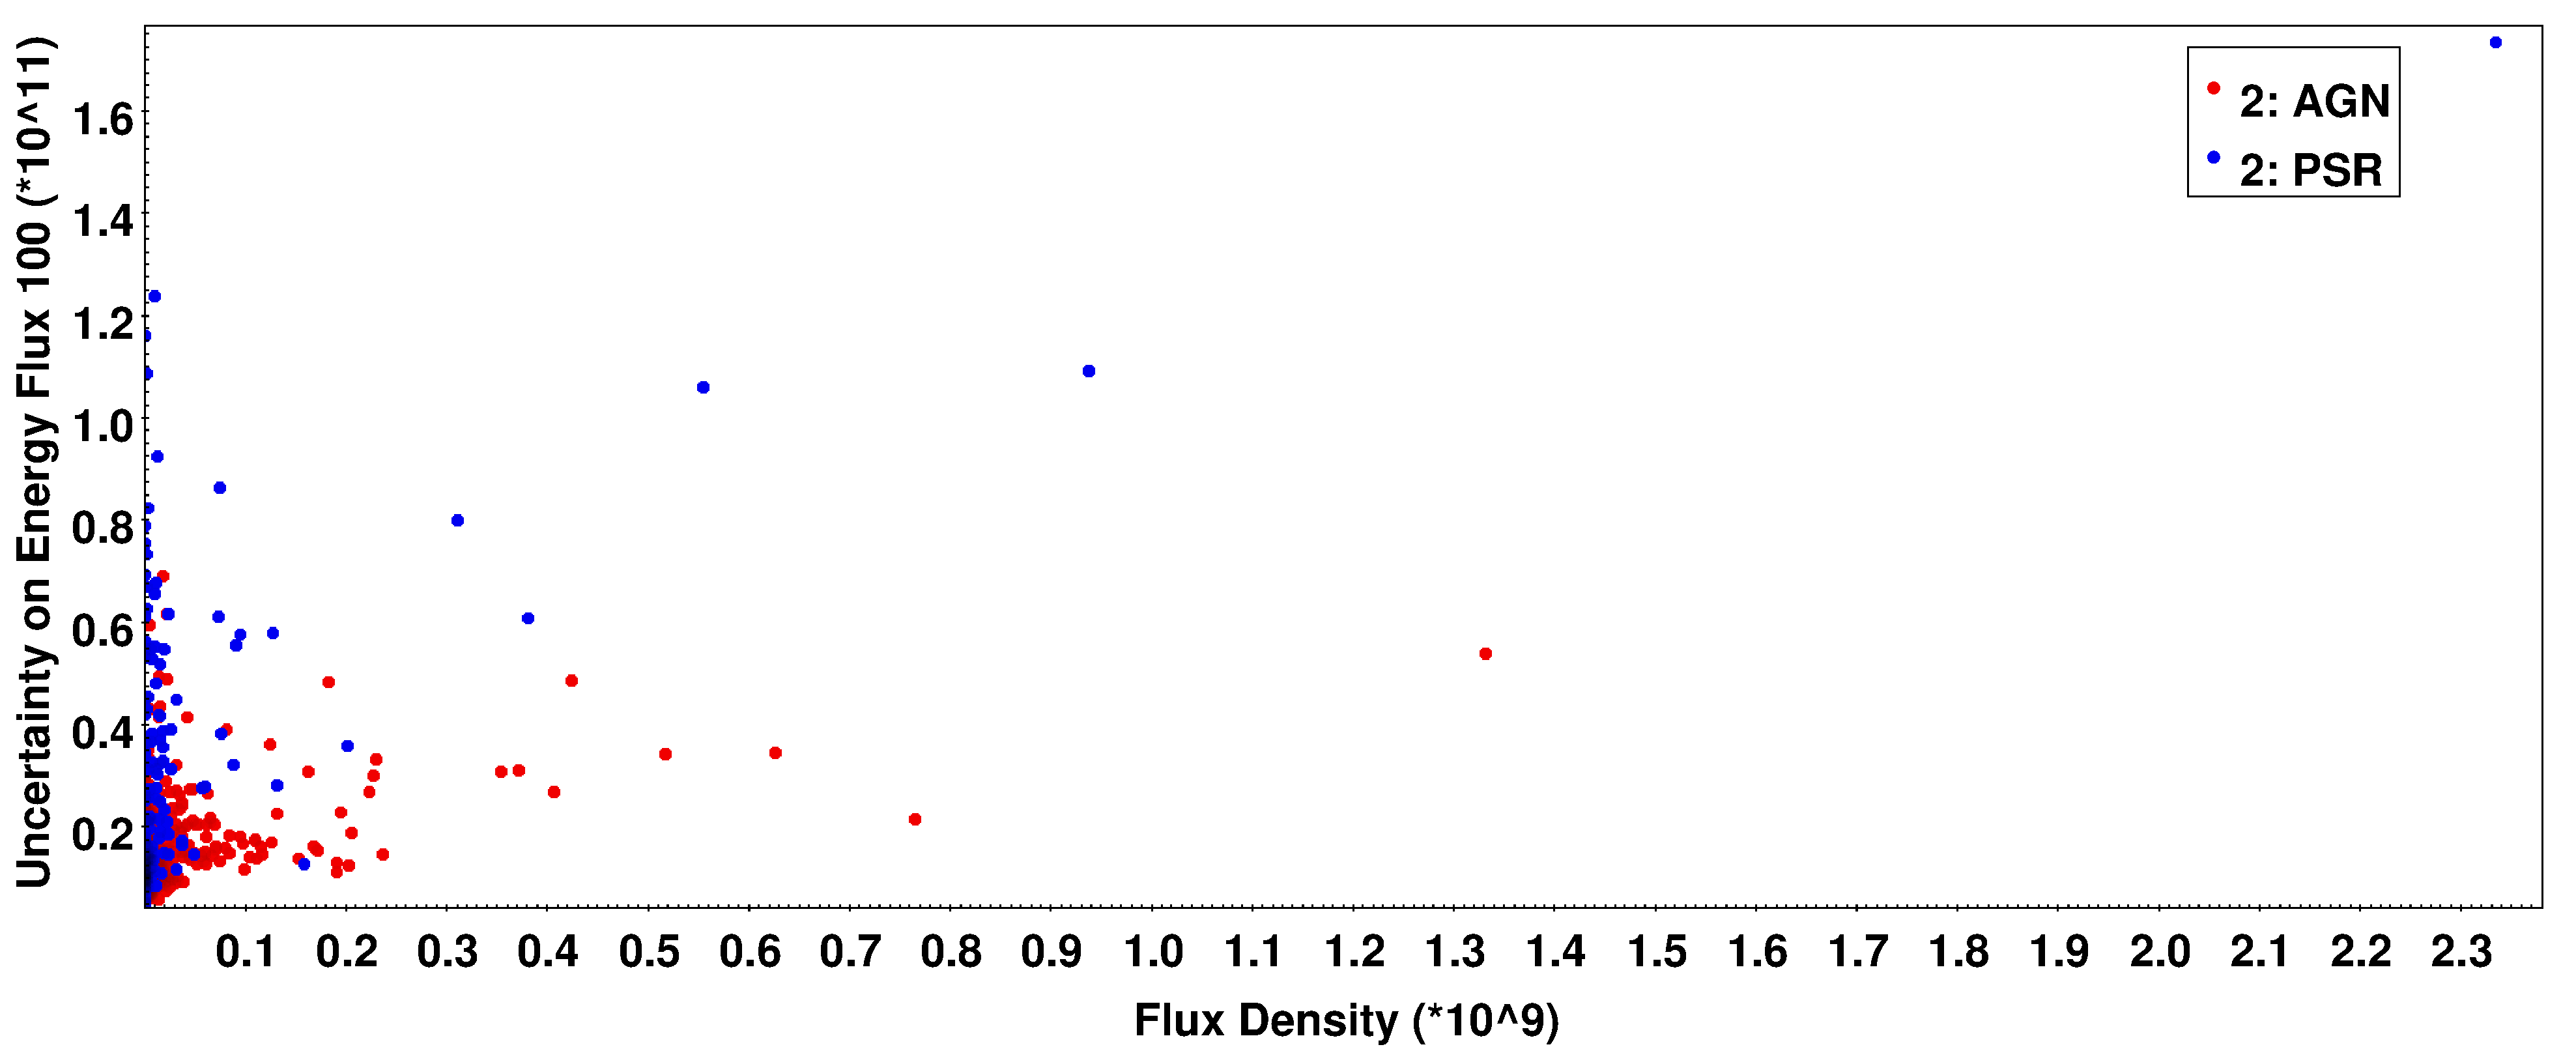
\includegraphics[width=\onepic\textwidth]{plots/fluxvsunc.pdf}
\caption{Separation of AGNs and PSRs from the 3FGL catalog based on different features}
\label{fig:corr}
\end{figure}




These importances were found to be consistent for various different algorithm parameters. So while the value might change a bit for different tree architechtures, for instance, the importances of these features were still pronounced. \\
\subsection{Comparison of the classification algorithms}

\end{comment}

\subsubsection{Random Forests}


\begin{figure}[h]
%\centering
\hspace*{-0.5cm}
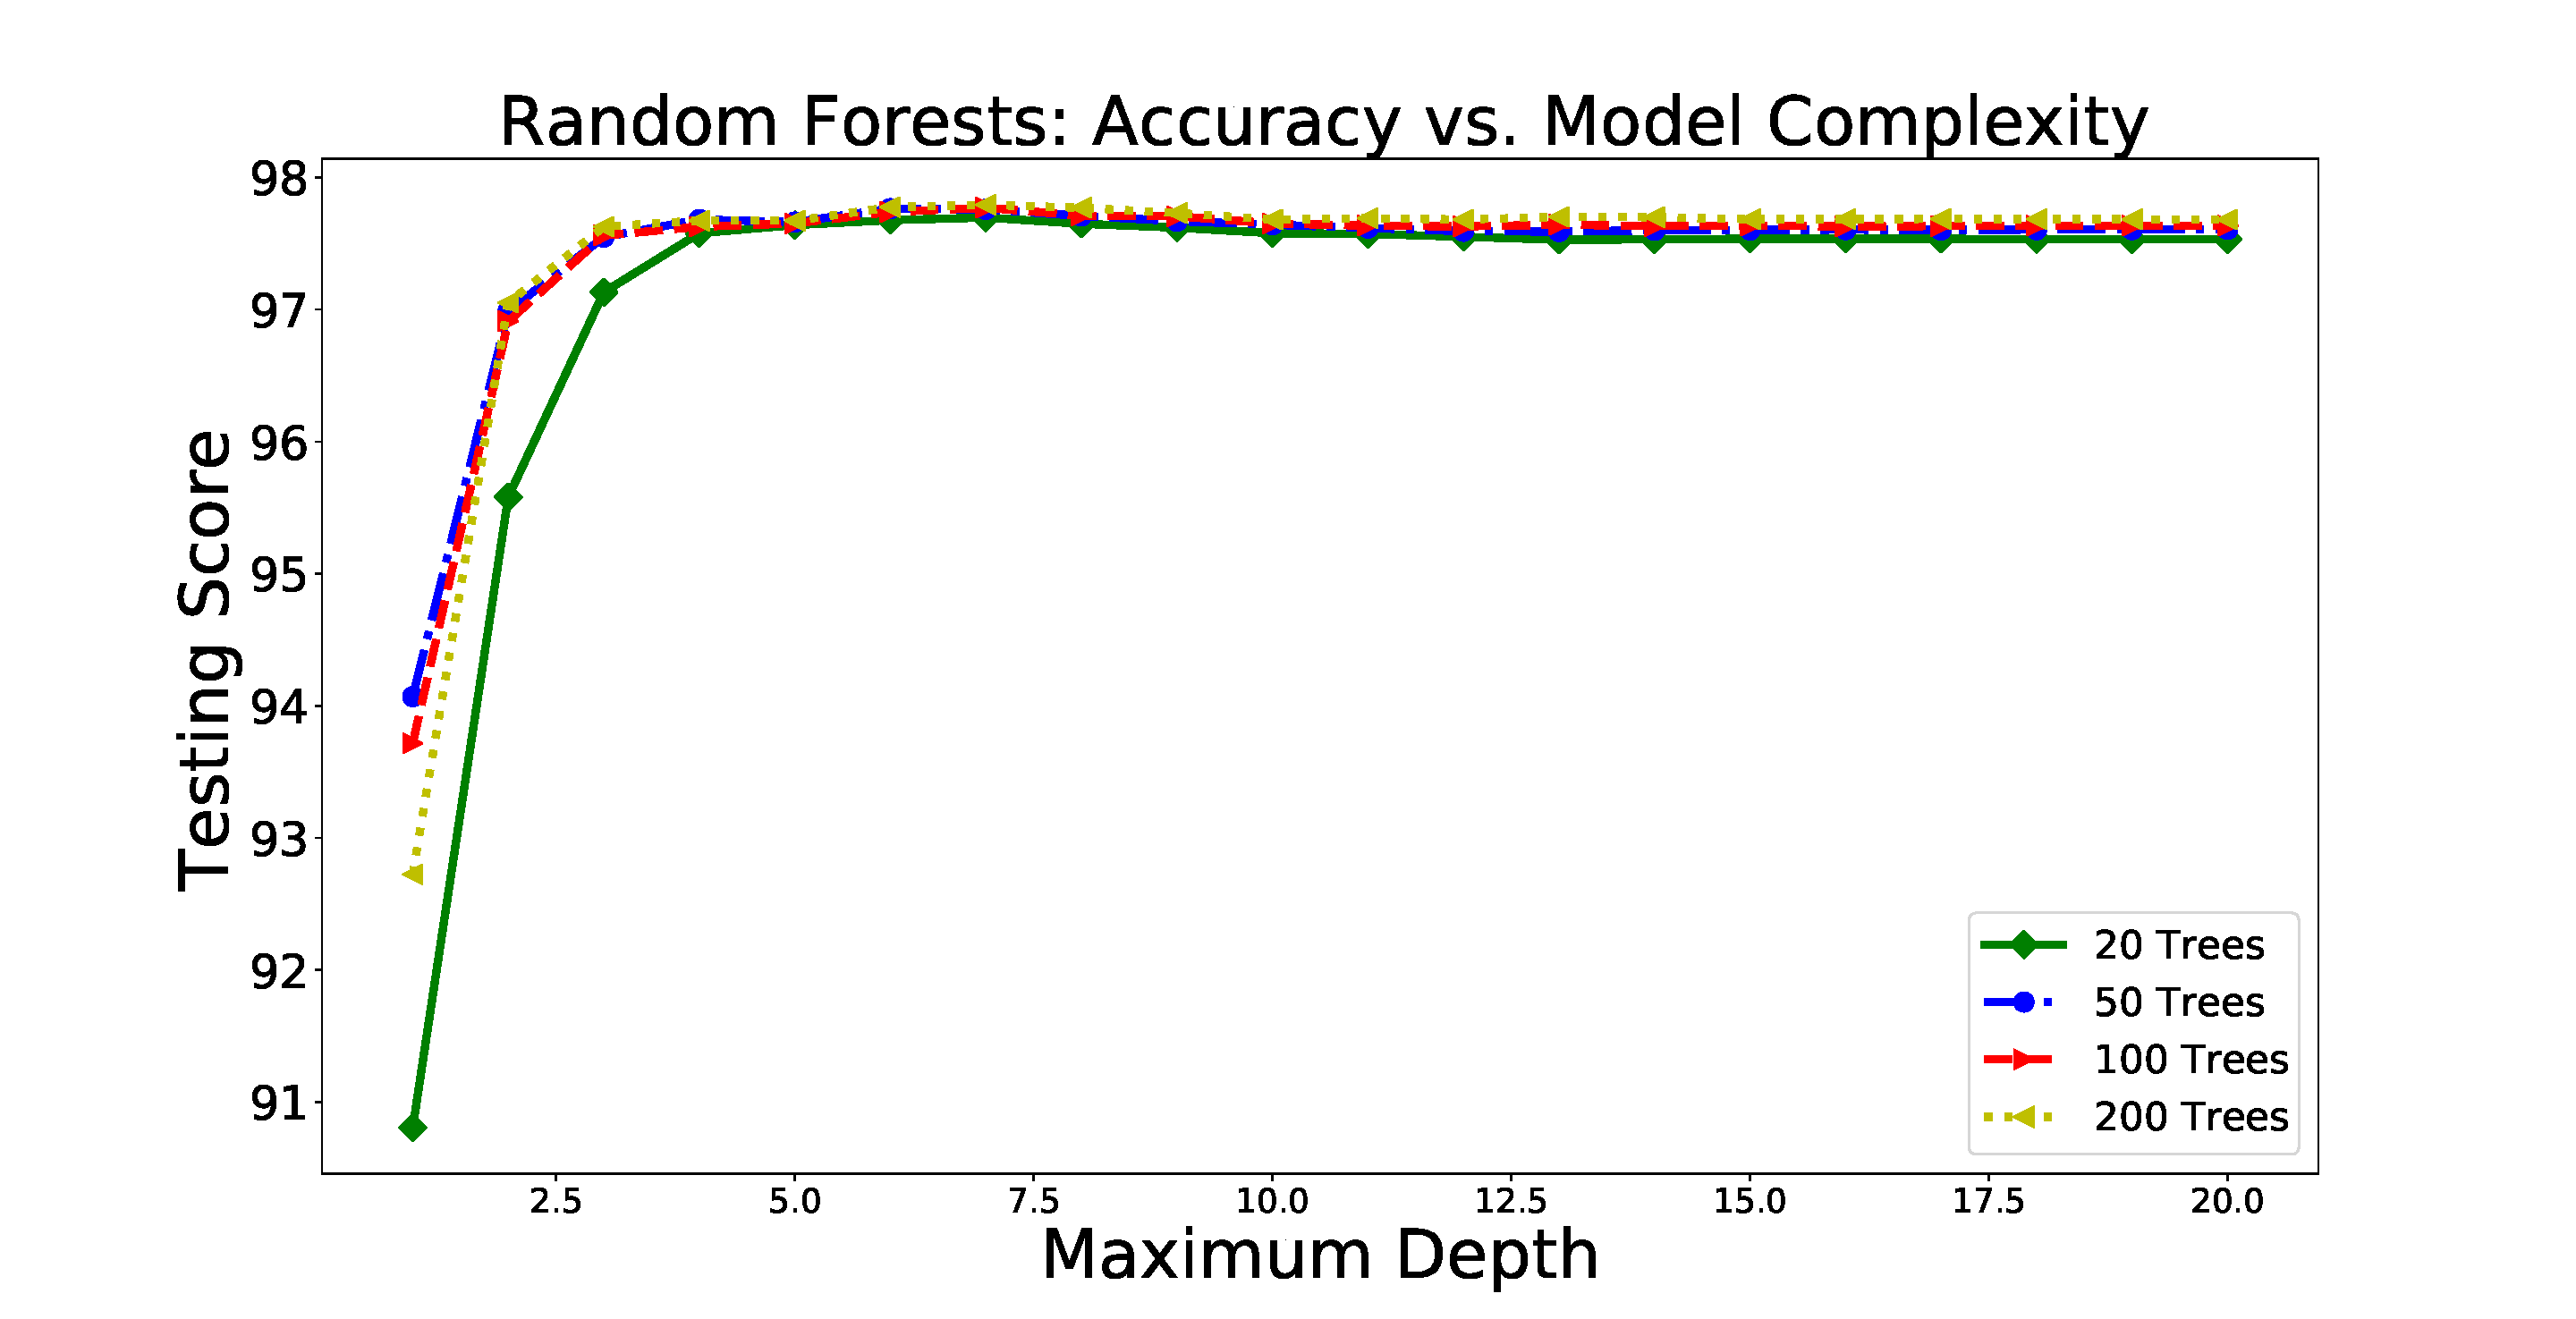
\includegraphics[width=0.5\textwidth]{plots/rf_train}
%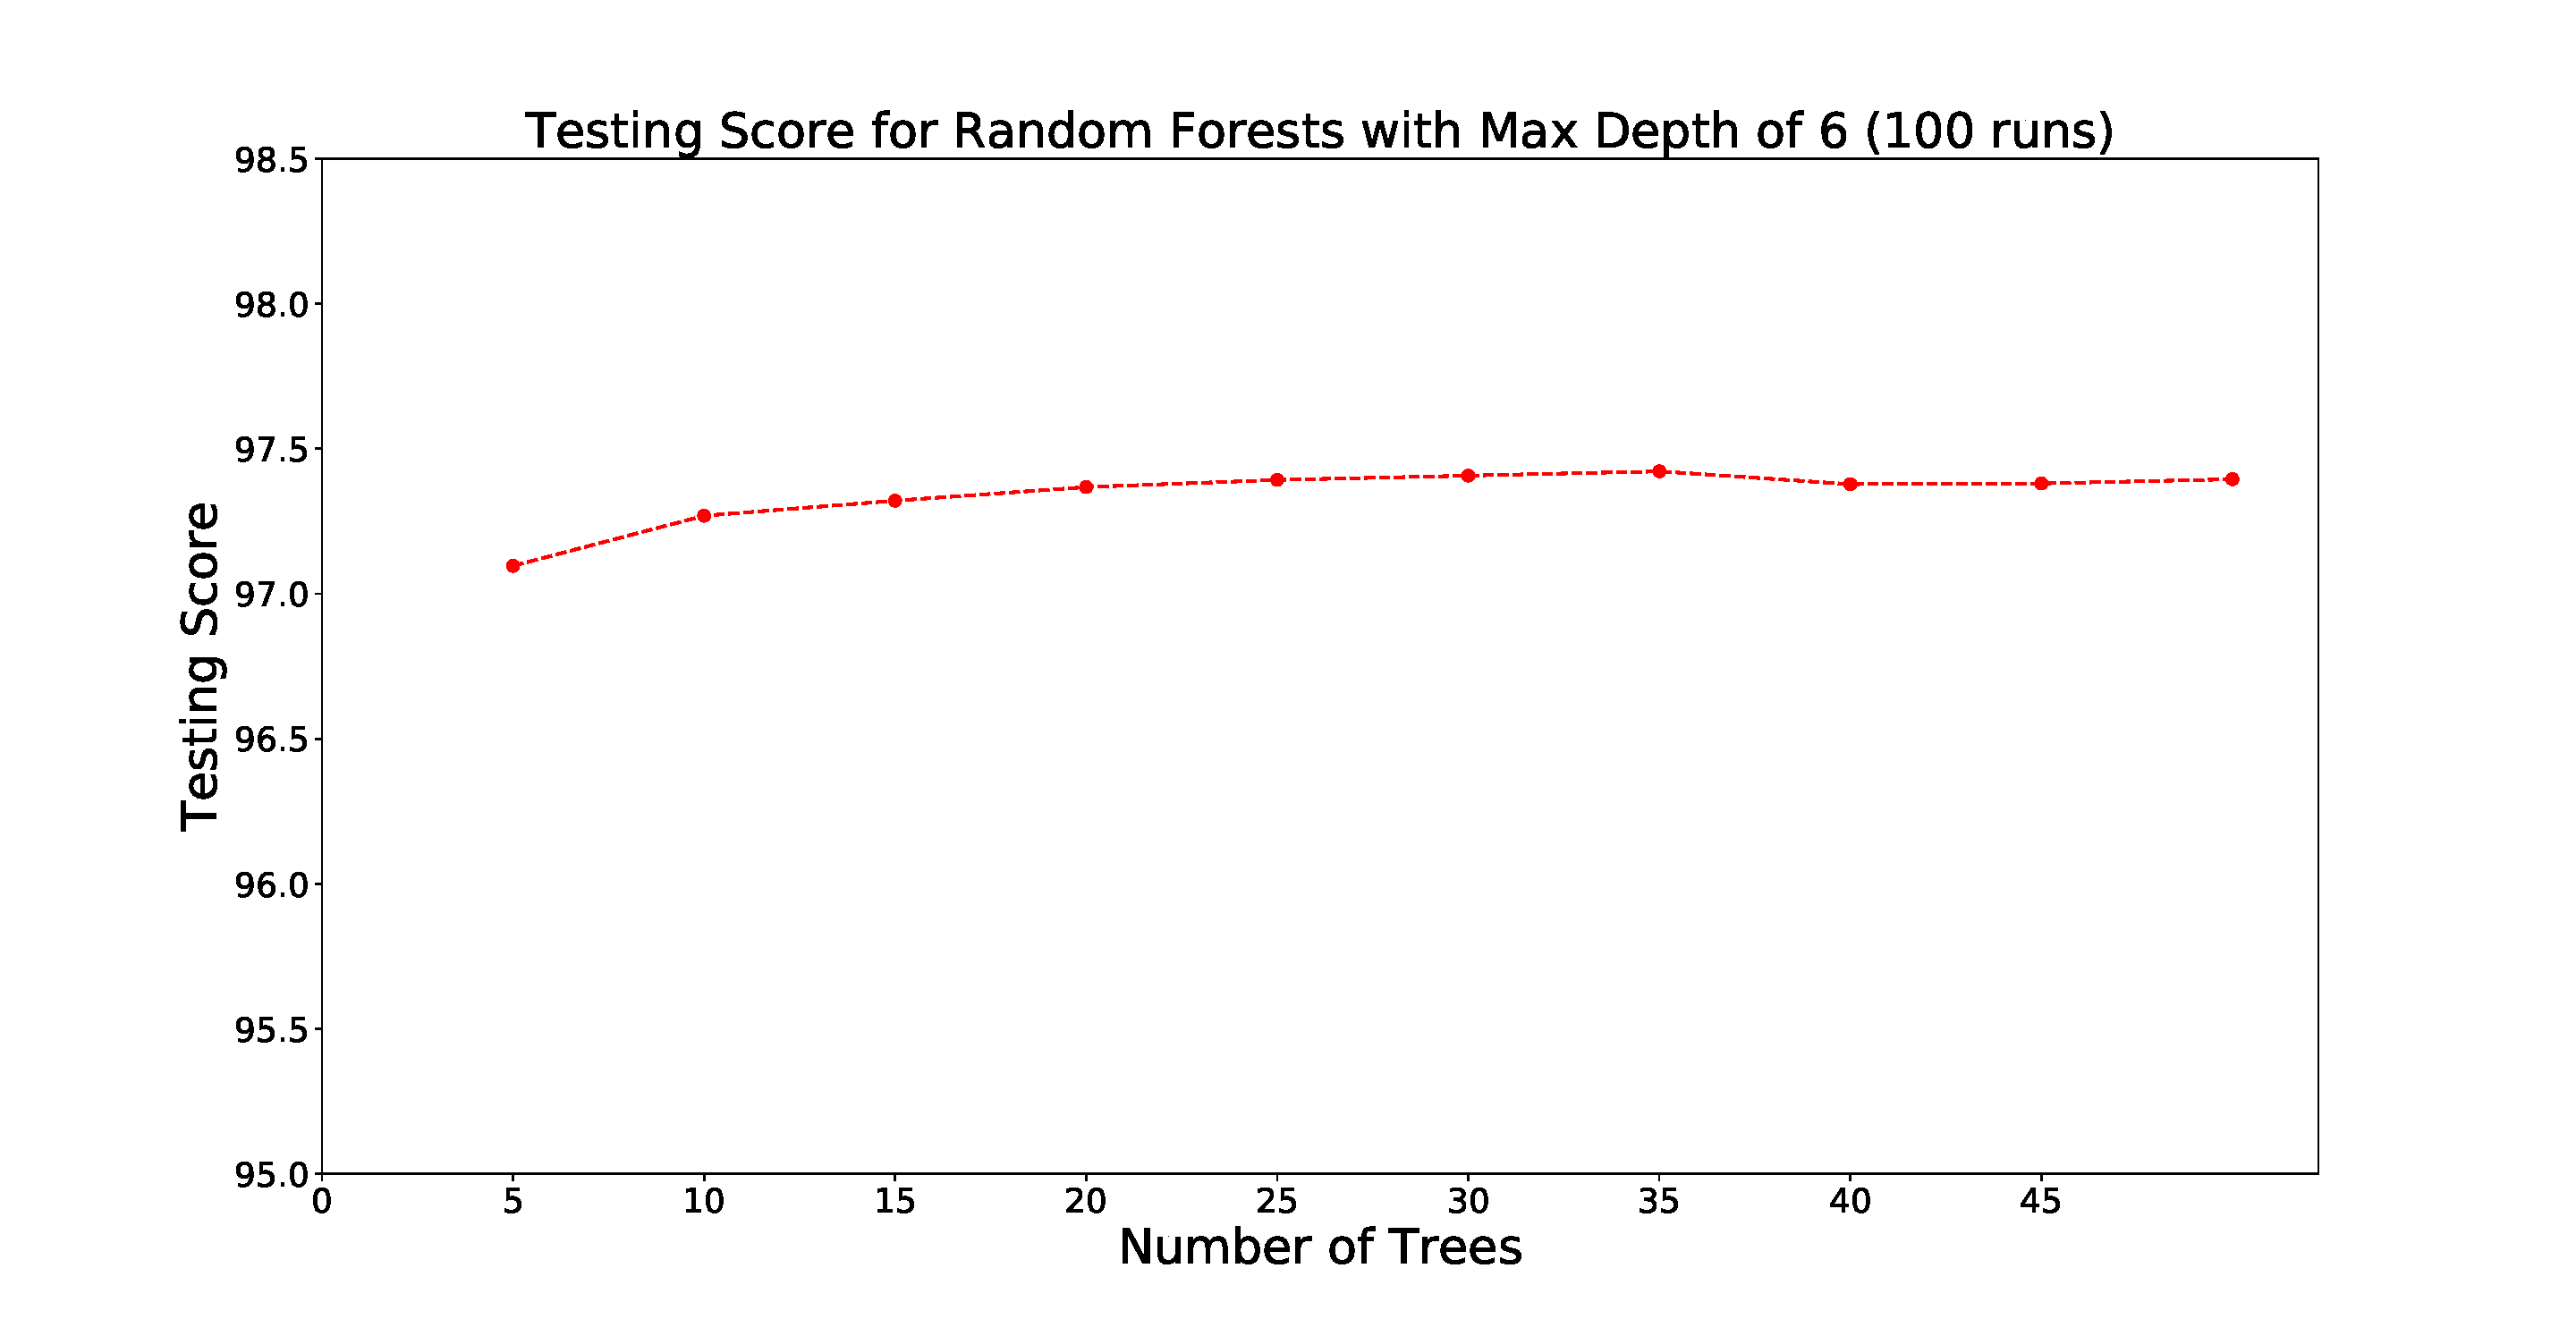
\includegraphics[width=\twopicsp\textwidth]{plots/6md_trees_weighted}
\caption{
Test score of RF classification as a function of the number of trees and maximal depth of trees.
%\dima{I think we should stop at 15 here since results don't change for max depth above 15.}
}
\label{fig:RF_complexity}
\end{figure}

The two main parameters characterizing the random forest algorithm are the number of trees and the maximum depth. 
Figure \ref{fig:RF_complexity} shows the dependence of the accuracy on the test sample as a function of maximum depth and the number of trees. For each line the number of trees is fixed.
The results for each point are averaged over 100 runs.
We have performed weighting the data by the inverse numbers of pulsars and AGNs to take into account that there are more AGNs than pulsars. Training on data without the inverse weighting did not have a significant effect on the accuracy.
We notice that the test score does not decrease with larger complexity of the model 
(larger number of free parameters due to larger maximal depth of trees).
This is due to the random choice of a subset of features at each node.
For the final algorithm, we will use a RF with 200 trees and a maximum depth of 8 trained on inversely weighted data. A depth greater than 8 results in a drop in performance. For the objective function we chose the gini index, which uses the square of the class probabililties for minimization.\\
%In the case of training, we found no significant differences when using weights for our data set. However, we chose to use a inversely weighted dataset since that allows us to generalize the algorithm more. The influence of weights will also be discussed more in the case of unassociated data, in the next section.
%After running tests on various architectures we chose a Random Forest with 20 trees to avoid over-fitting, and a maximum depth of 12.
%\dima{
%Why 12? It looks like 4 or 5 is already good enough.
%We should write here an equation for test score in case of weighted data.}

In tree-based algorithms, one can calculate feature importance by using the averaged reduction of impurity for nodes involving the different features. The feature importances for the case of two different RF algorithms: 20 trees with max depth 12 and 50 trees with max depth of 6 are shown in Table \ref{tab:feat_imp}.
We find that the four most important features are spectral curvature, hardness ratio of the last two energy bins, spectral index, and variability, which follow the trend regardless of hyper-parameters chosen.
%Since Random forests are based on decision trees, they allow us to characterize feature importances based on how helpful a feature was to split a tree. In our case, using all 10 features discussed above we found the following feature importances for two architectures of random forests with similar accuracies of 97.5:\\


\begin{table}[!h]
    \tiny
    \centering
    \renewcommand{\tabcolsep}{1mm}
\renewcommand{\arraystretch}{1}

    \begin{tabular}{|c|c|c|}
    \hline
    Feature &  20 trees, depth 2& 50 trees, depth 6\\
    \hline
    Flux Density& 0.04 & 0.05        \\
    \hline
    Unc Energy Flux100& 0.07     & 0.08 \\
    \hline %\midrule   -> aakash do you mean this?
   Spectral Index & 0.13     &   0.11\\
    \hline %\midrule   -> aakash do you mean this?
    Significant curvature& 0.33 &0.29  \\
    \hline
   var&  0.06   &  0.10  \\
    \hline %\midrule   -> aakash do you mean this?
    hr12& 0.03 &0.03 \\
    \hline
     hr23& 0.03 &0.04 \\
    \hline
    hr34& 0.02 &0.03 \\
    \hline
   hr45& 0.25 &0.21 \\
    \hline
    GLAT&0.01&0.02\\
    \hline
    \end{tabular}
    \vspace{0.4cm}
    \caption{Feature importances for two RF algorithms.}
    \label{tab:feat_imp}
\end{table}

%Our hypothesis about feature importances turned out to be correct, as curvature, variability, and spectral index were the most important features. The last hardness ratio was also seen to be quite important, most probably reflecting the end of the spectrum where the AGNs and PSRs shift from each other.\\

In order to illustrate the separation of the PS into AGNs and pulsars, we retrain the RF algorithm using only two features: curvature significance and spectral index, and plot the resulting probabilities of classes in Figure \ref{fig:RF_domains}. These classification domains provide us with a look at the complexity of the network. As we can see the depth 4 outperforms depth 2. We decide to go higher on the depth and trees, since this plot is a 2-d estimation of a 10 feature problem, as we have only plotted for two of the main features. As can be seen in the figure, the colourer is redder closer to cluster of AGNs and bluer in areas with higher PSRs. The probabilities are shown for only one run, as a way of illustrating how the algorithm seperates different regions of the data-set. The higher the depth the more the probabilities becomes denser and the dense areas become smaller. For instance, one can see region of near zero probabilities in the depth of 4, as opposed to a depth of 2.  
\dima{Add discussion of the domains, e.g., overfitting, and selection of the final model for classification.}

\begin{figure}[h]
\hspace*{-1.5cm}
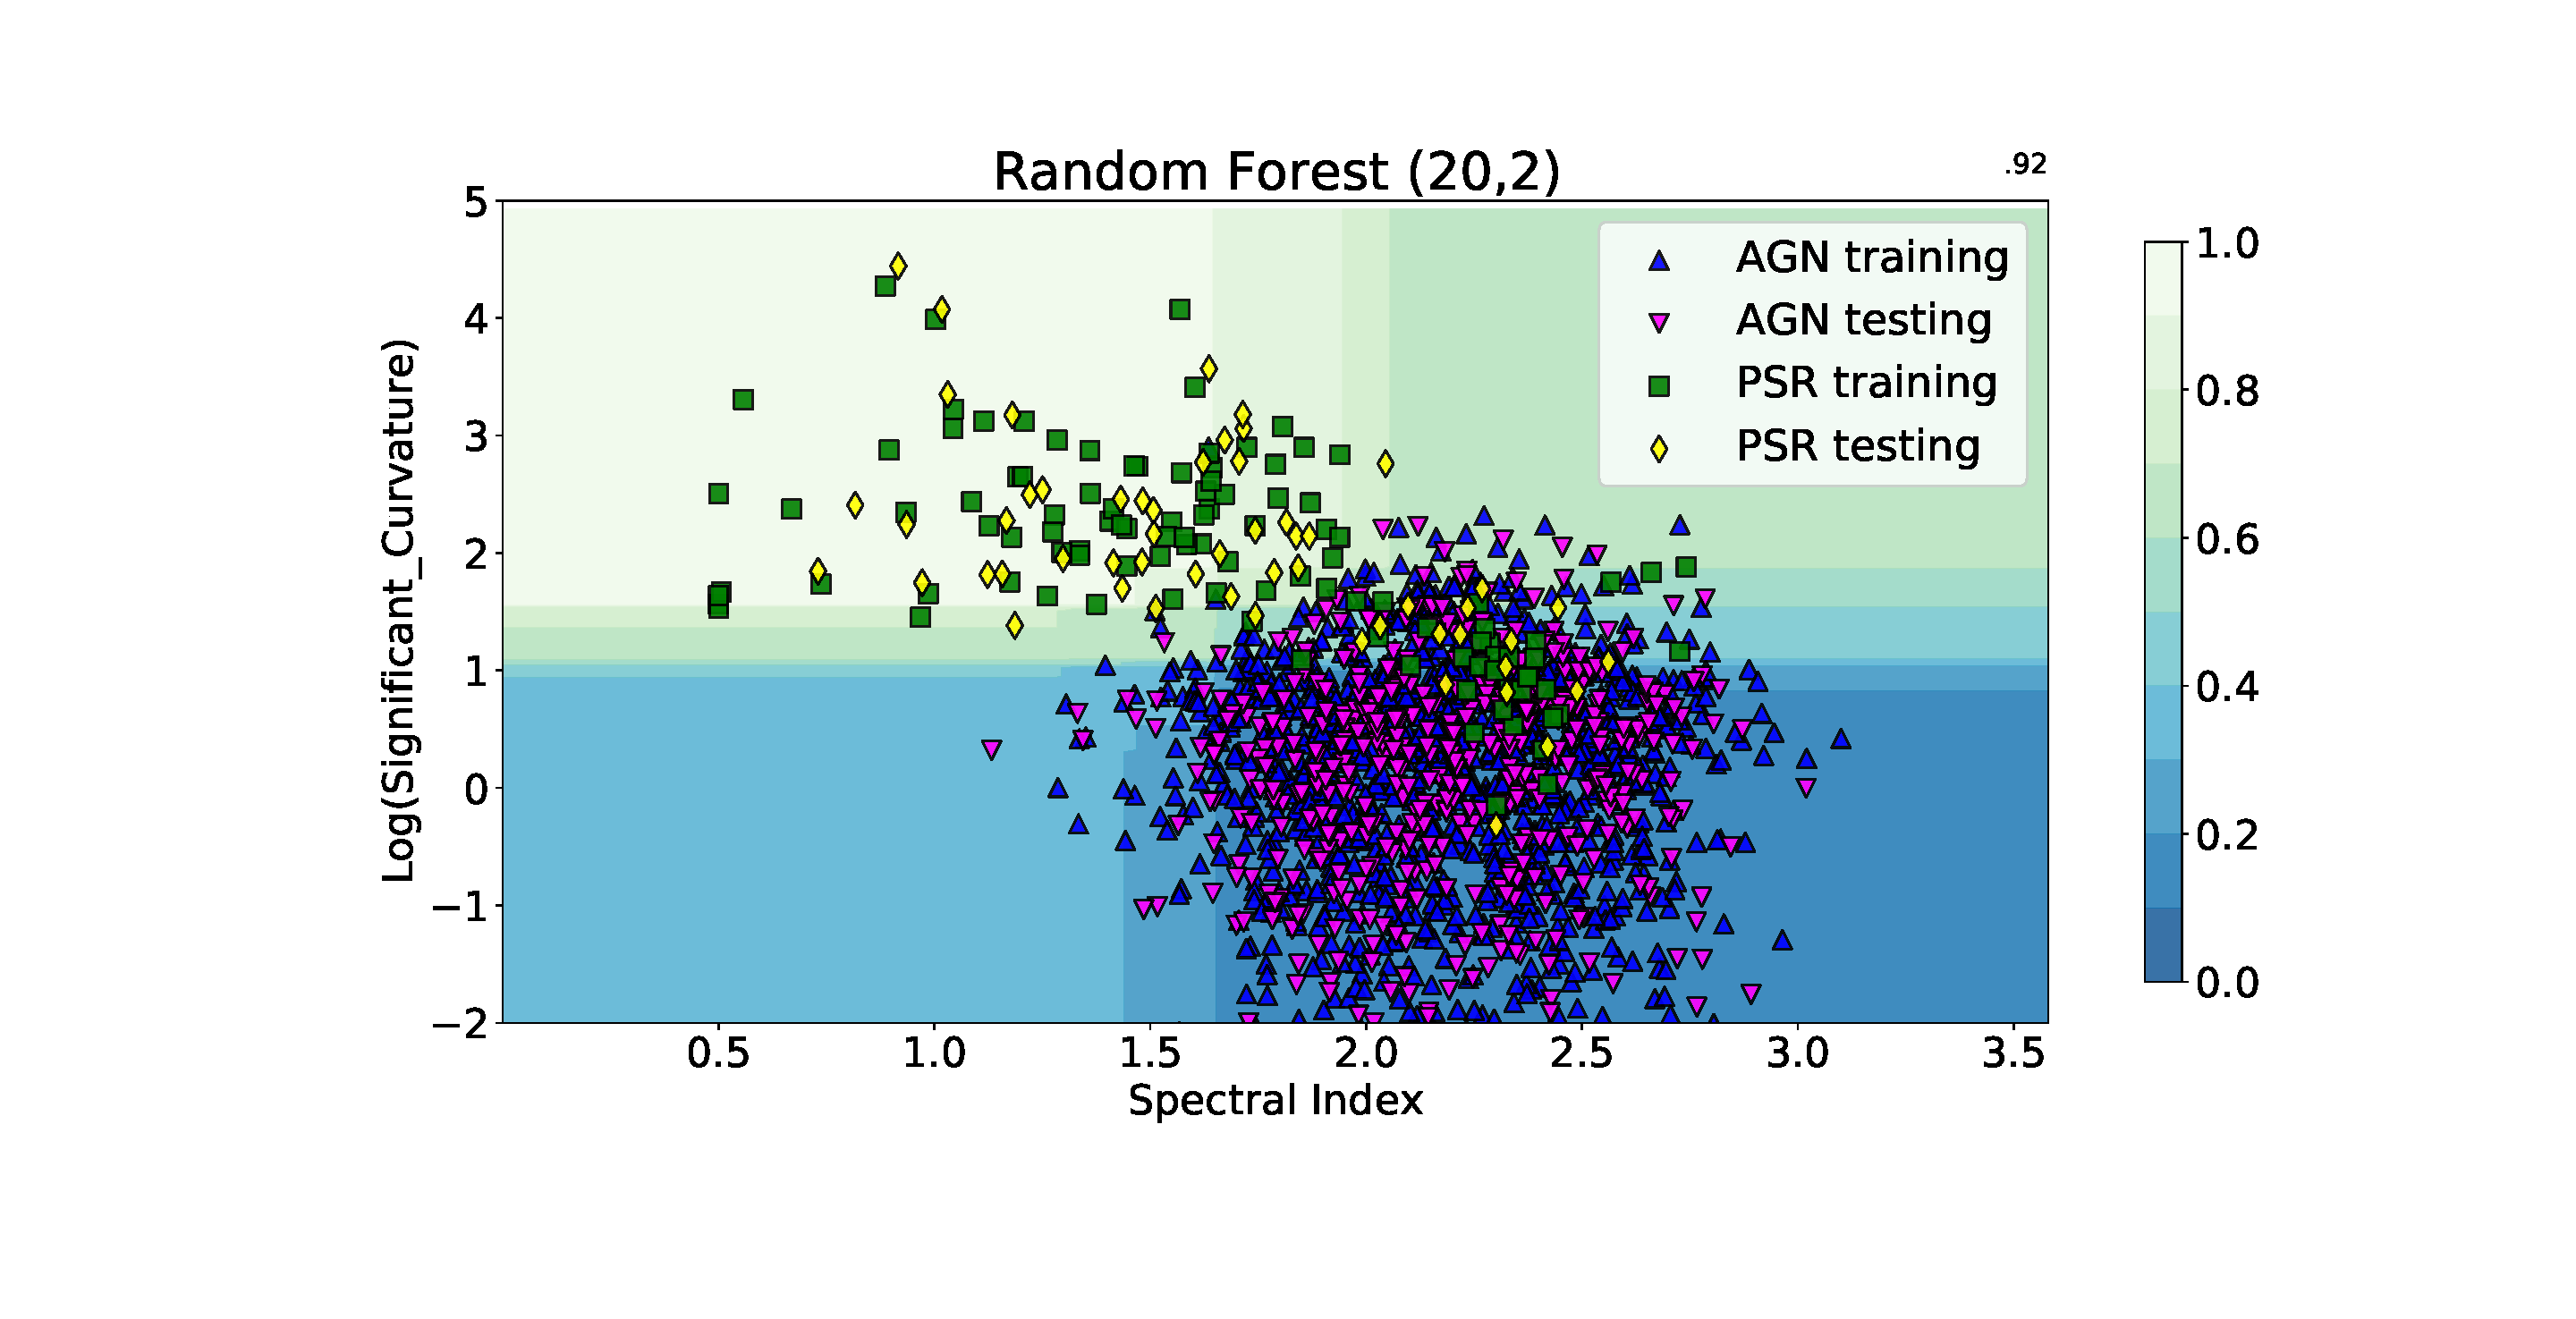
\includegraphics[width=0.6\textwidth]{plots/classification_domains/rf_20_2_final.pdf}
\hspace*{-1.5cm}
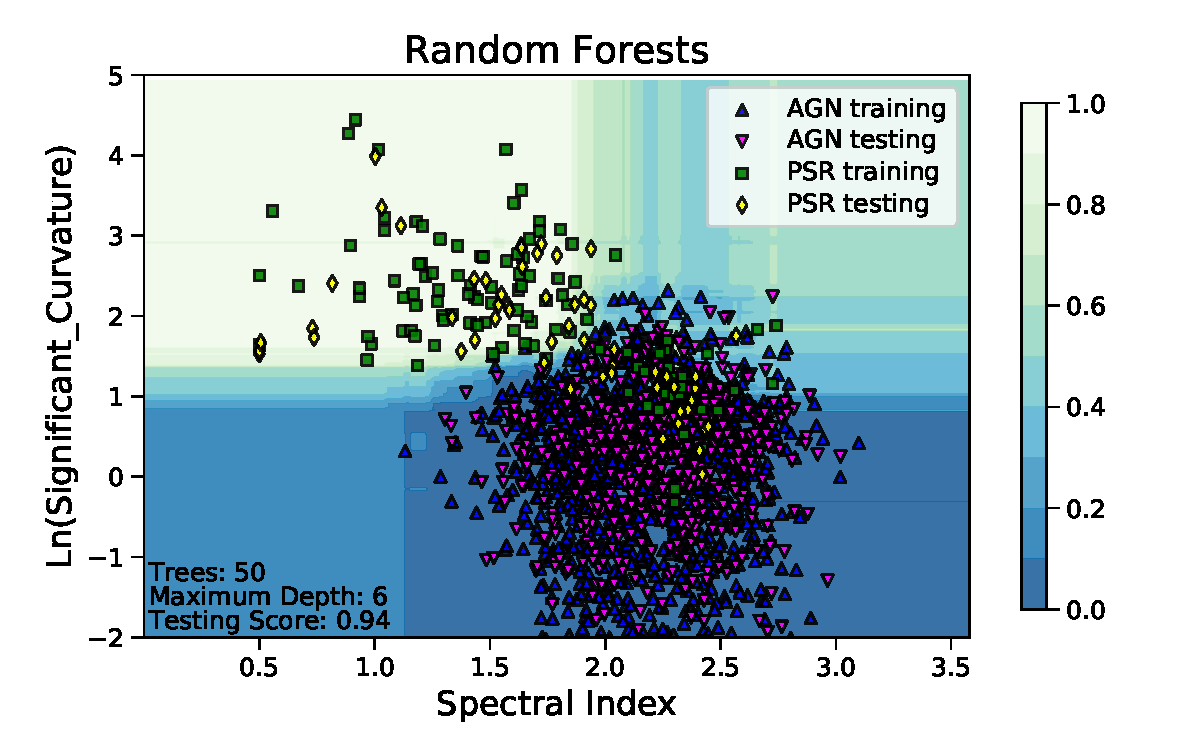
\includegraphics[width=0.6\textwidth]{plots/classification_domains/rf_50_6_final.pdf}
\caption{Classification Domains of RF: Differences in decision function for lower model complexity, compared to the chosen model.}  
\label{fig:RF_domains}
\end{figure}

%=======
%\begin{figure*}[h]
%\centering
%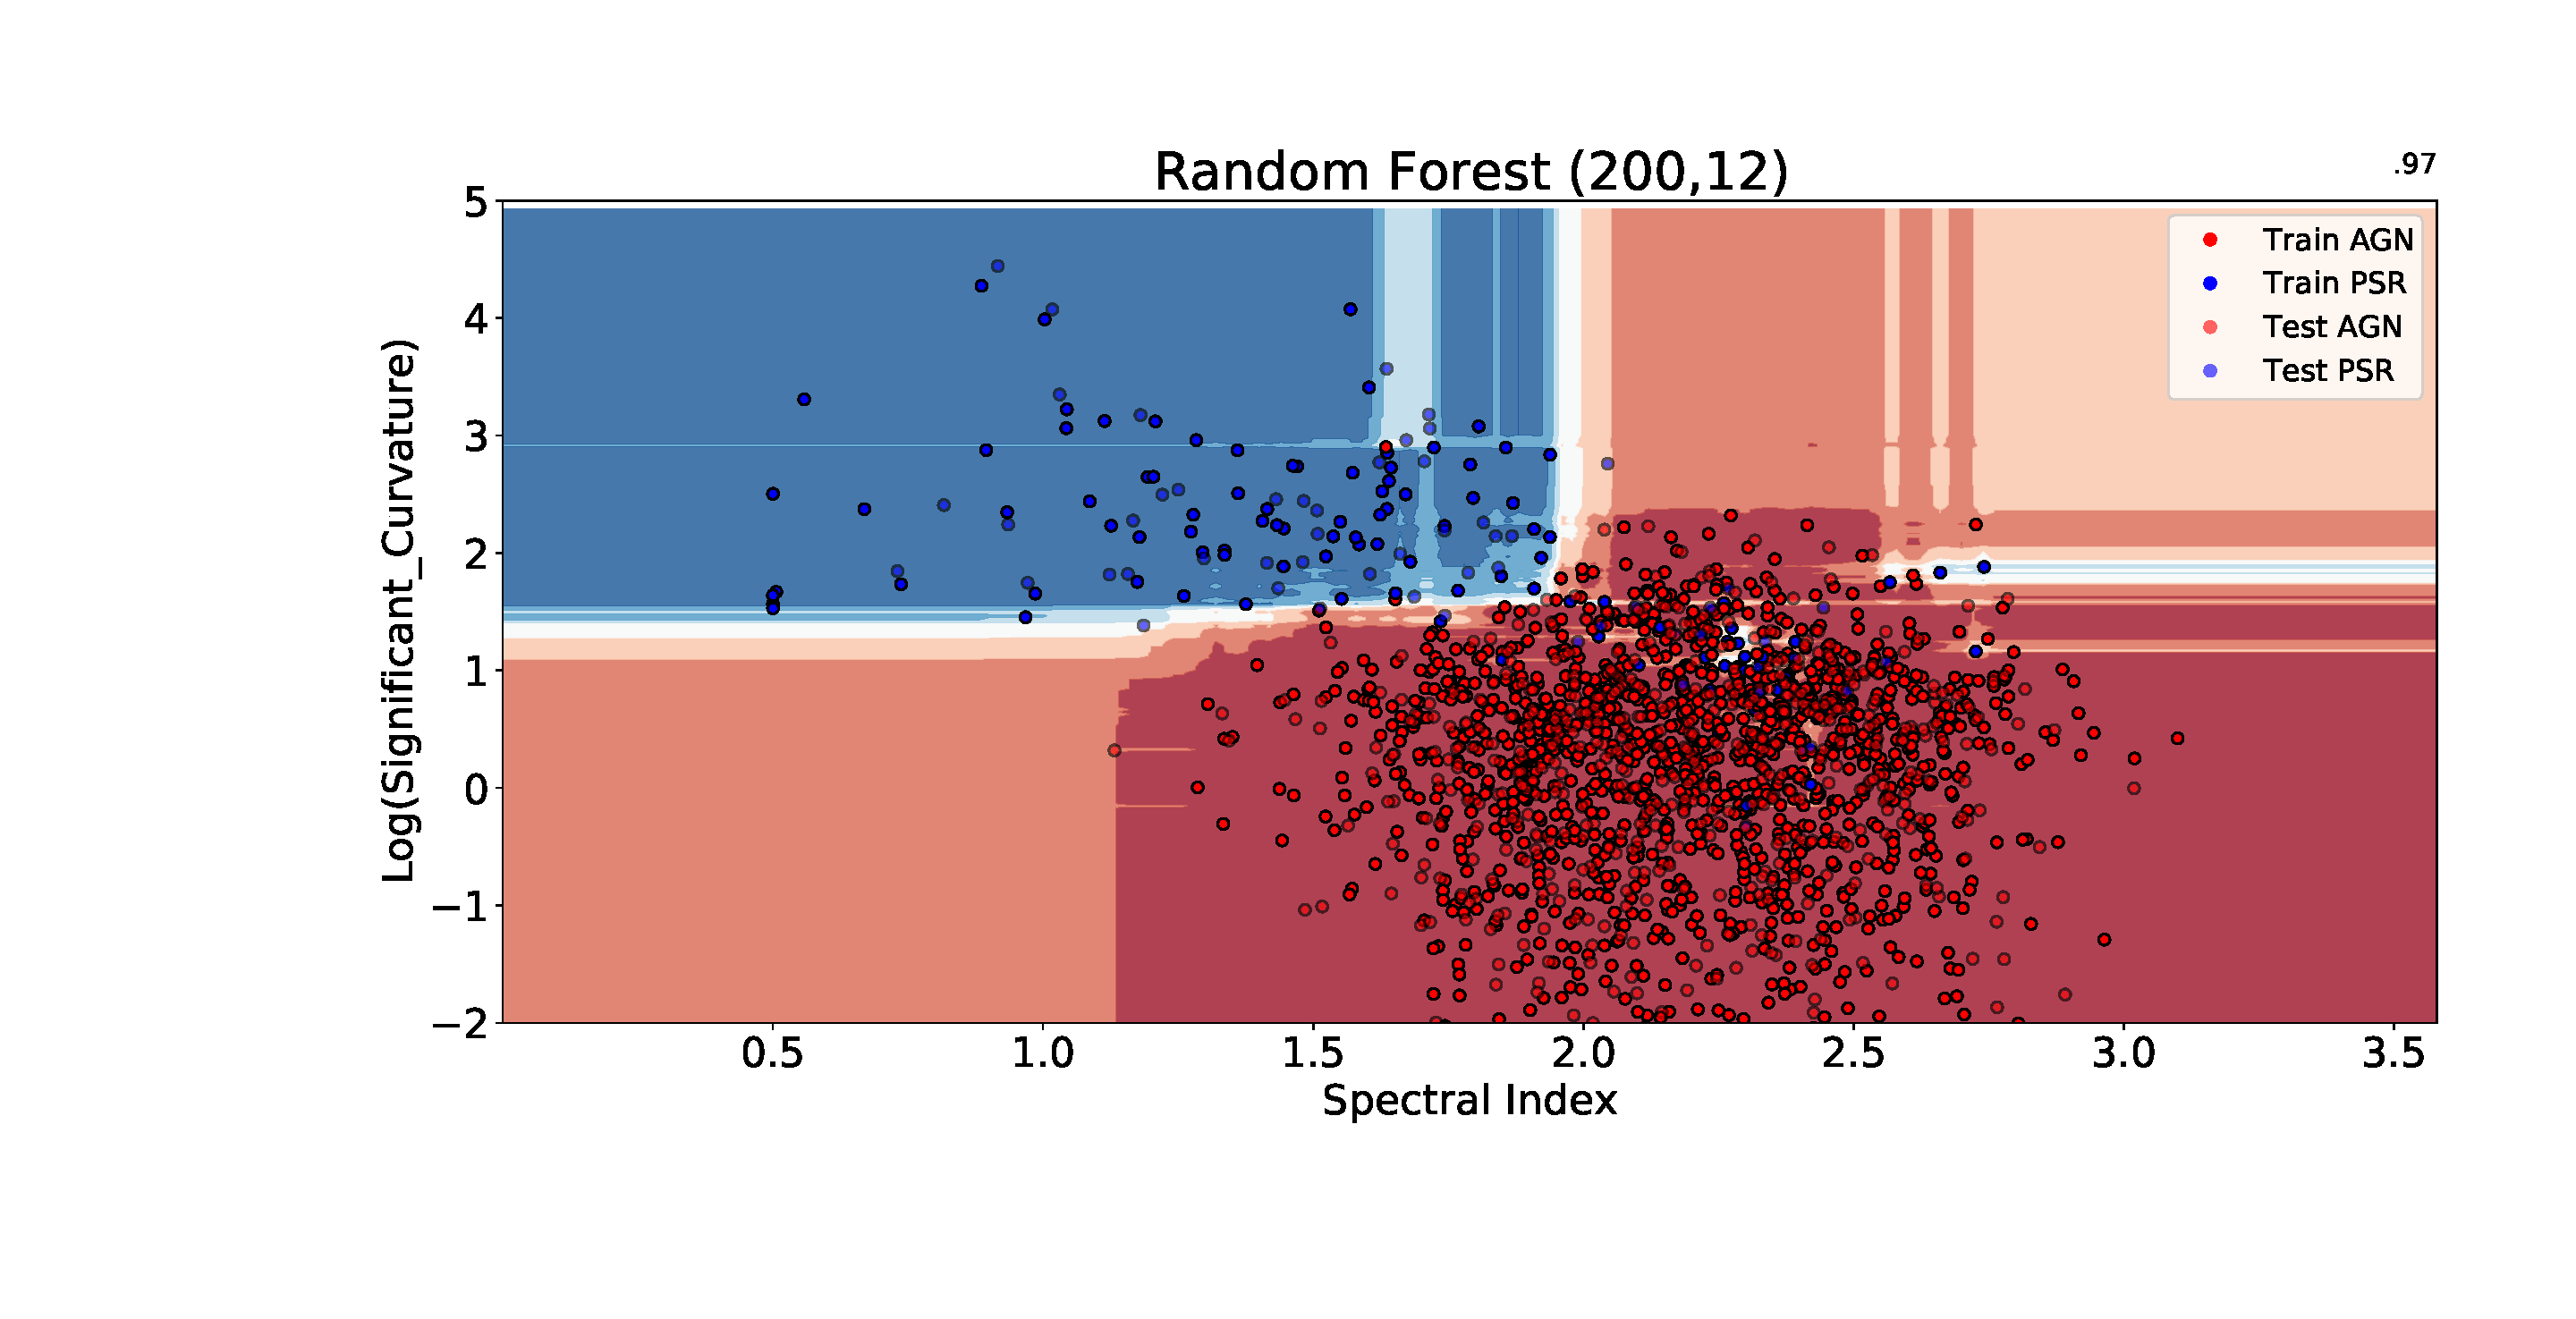
\includegraphics[width=\twocolumnwidth\textwidth]{plots/classification_domains/rf_200_12.pdf}\\
%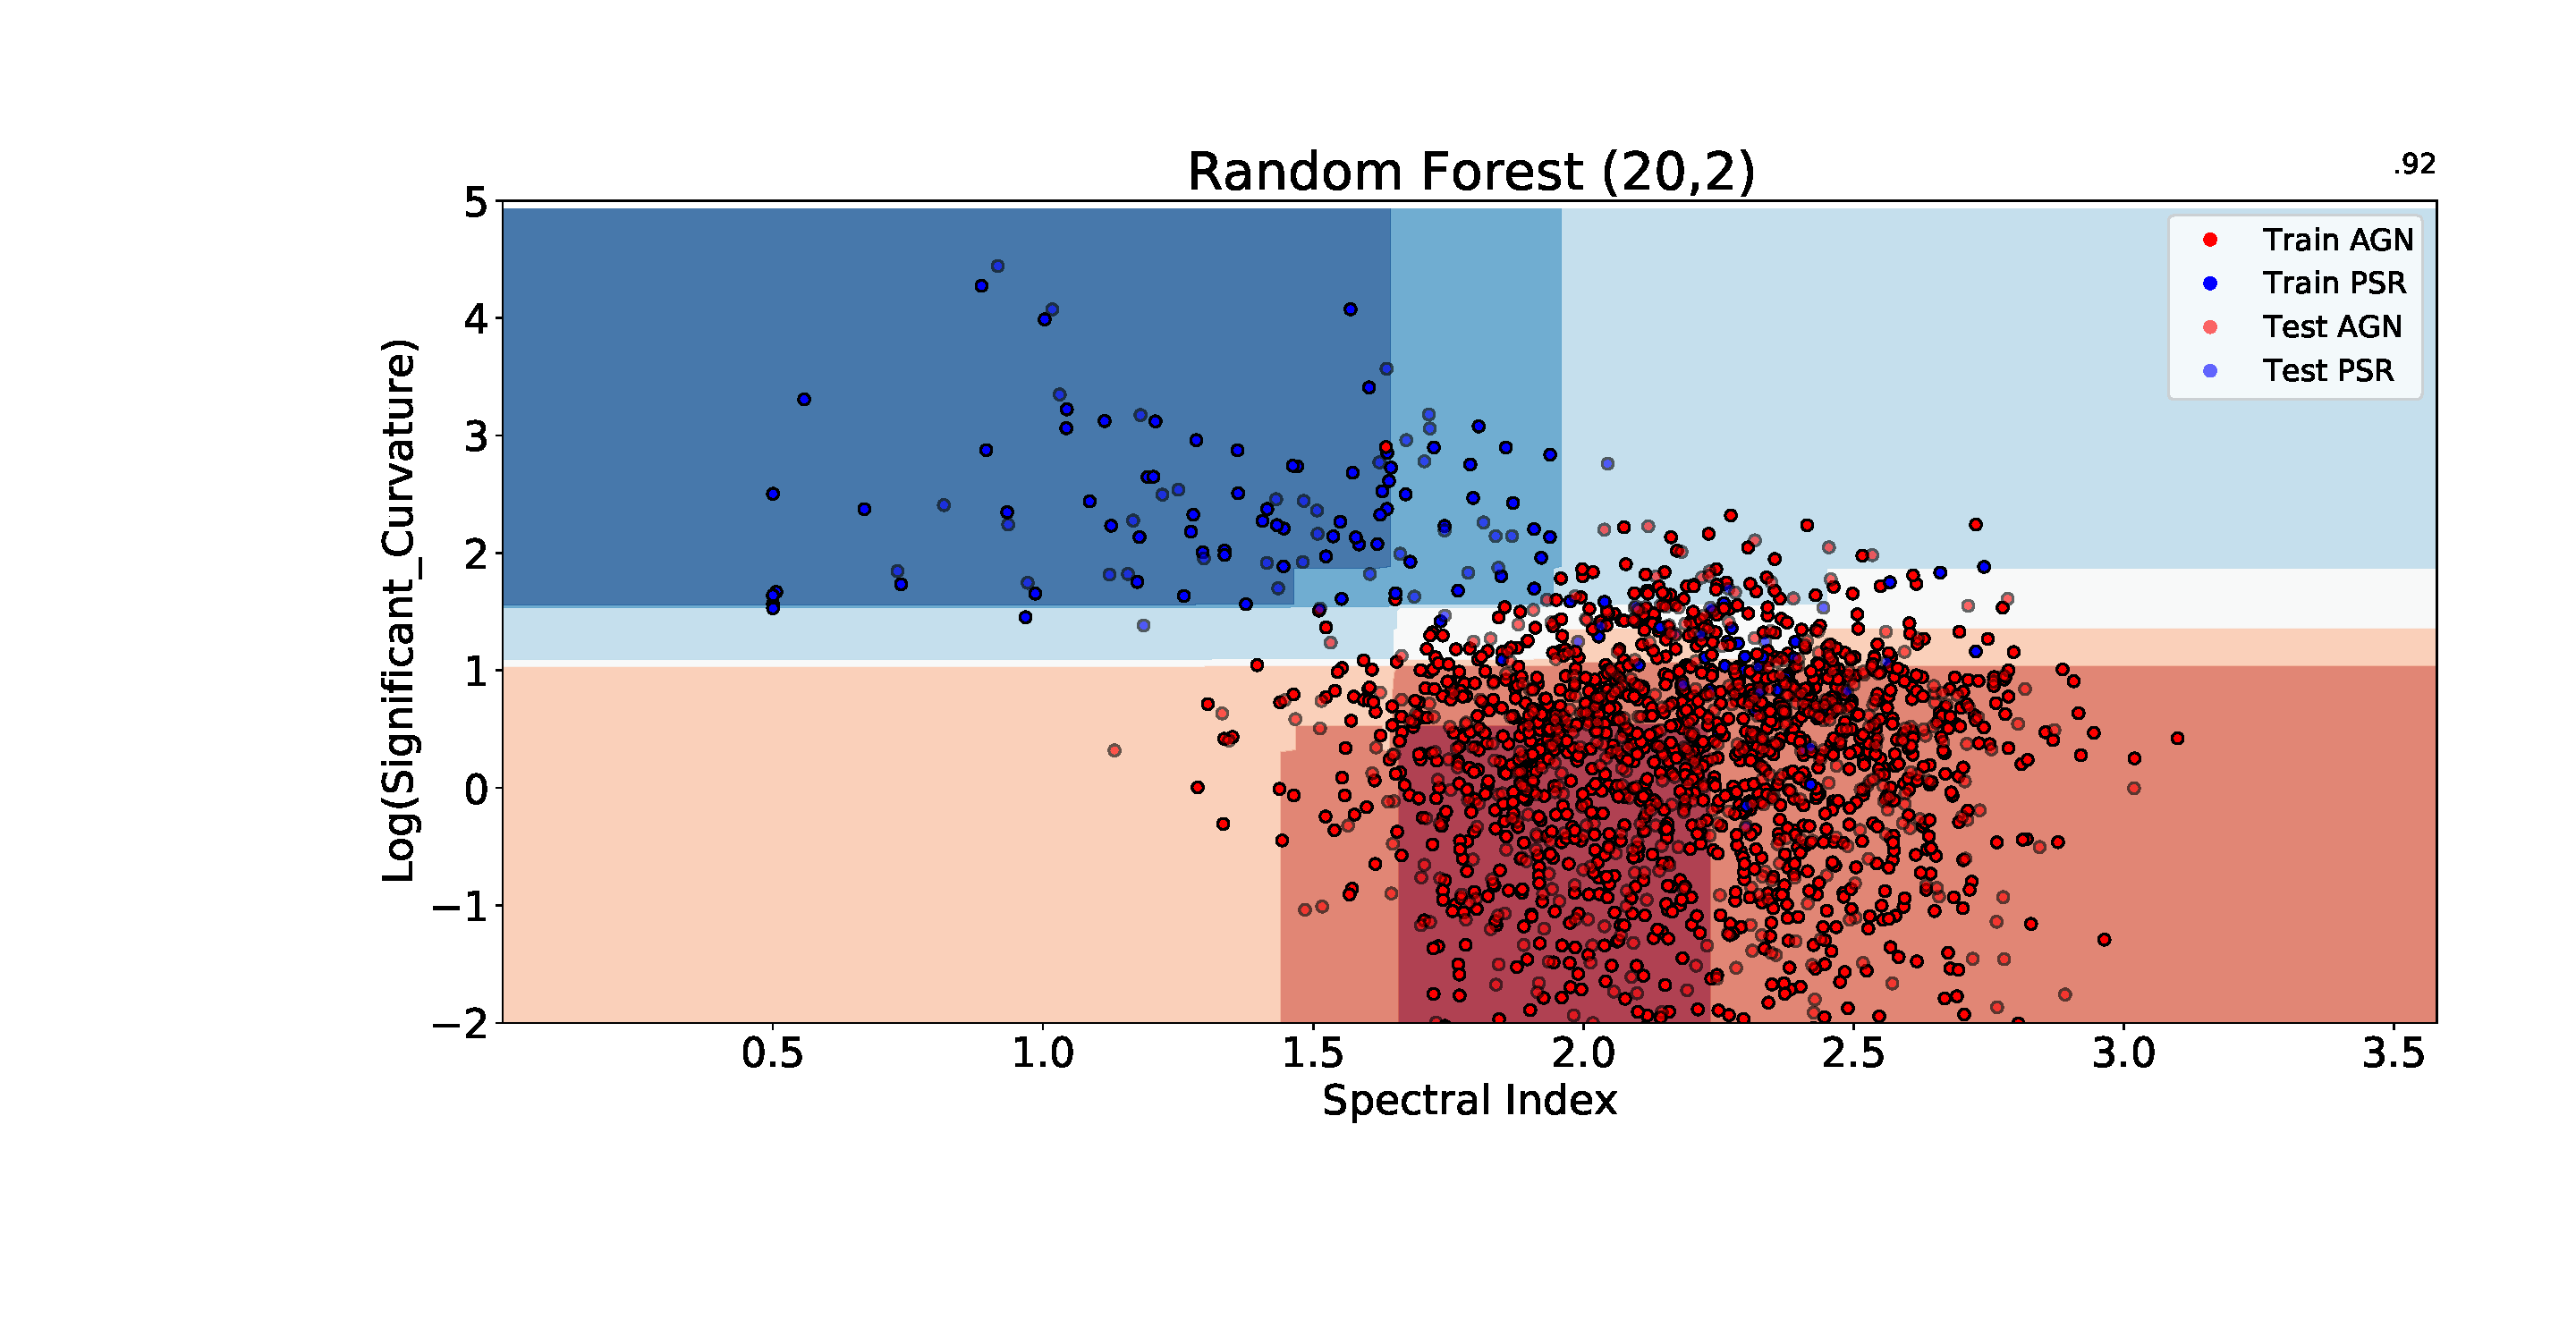
\includegraphics[width=\twocolumnwidth\textwidth]{plots/classification_domains/rf_20_2.pdf}
%>>>>>>> a522eecb66fa0cf6f440bc2907db2c42d74cac67
%\caption{Classification Domains of RF.  \dima{Why don't we show the domains for the final model, which we use for predictions?
%Moreover, it looks like for max depth 12 the model overfits the data, i.e., using max depth of 4 or 5 would be better for the final model.
%We should also add color bars for all domain plots and make the labels larger.}}
%\label{fig:RF_domains}
%\end{figure*}


\subsubsection{Neural Networks}

In the case of NN, the number of free parameters depends on the number of hidden layers and on the numbers of nodes.
Adding more than one hidden layer did not improve the accuracy of the classification.
In the following we will use NNs with only one hidden layer.
Dependence of the accuracy for test sample on the number of neurons in the hidden layer is shown in Figure \ref{fig:NN_neurons}.
Dependence on the number of epochs (number of iterations in fitting) is presented in Figure \ref{fig:NN_epochs}. 
The methods used to solve the loss function are L-BFGS and ADAM. L-BFGS (Limited memory Broyden-Fletcher-Goldfarb-Shanno) is an approximation of the quasi-newtonian BFGS method. The BFGS method uses the full inverse of the nxn Hessian matrix to find the direction of movement for minimizing the gradient. The limited memory counterpart however, only stores a smaller representation of the full matrix. This makes this method much faster for larger data-sets.\\
ADAM on the other hand belongs to a realtively newer family of algorithms which use gradient descent. Gradient descent is a first-order method to find the local minima or maxima of a differentiable function. Nowadays, this process is made more efficient by taking the gradient from parts of the data-set instead of the entire data-set itself. This is called stocahstic gradient descent, since the data is selected randomly. ADAM is a newer approach of the stochastic family using adaptive network learning rates for every parameter. ADAM is usually preferred for Neural Networks with big data-sets.\\ 
%\dima{Discuss L-BFGS and ADAM methods here. I don't understand where you can use tanh and relu activations, if we have only one hidden layer with classification for output.}

\begin{comment}
 we were concerned with the number of epochs that one would need to tweak, along with a dependence on the number of neurons in the hidden layers. A final improvement involved checking whether multiple hidden layers would actually add to such a classification algorithm or not.\\
As can be seen in the figure, with the specific stochastic gradient method ADAM, the number of epochs required are higher since ADAM converges slow. However, after around 200 epochs the accuracy saturates and reached the same as the lbfgs solver, which converges faster for smaller data-sets. \\
\end{comment}

\begin{figure}[h]
%\centering
\hspace*{-0.5cm}
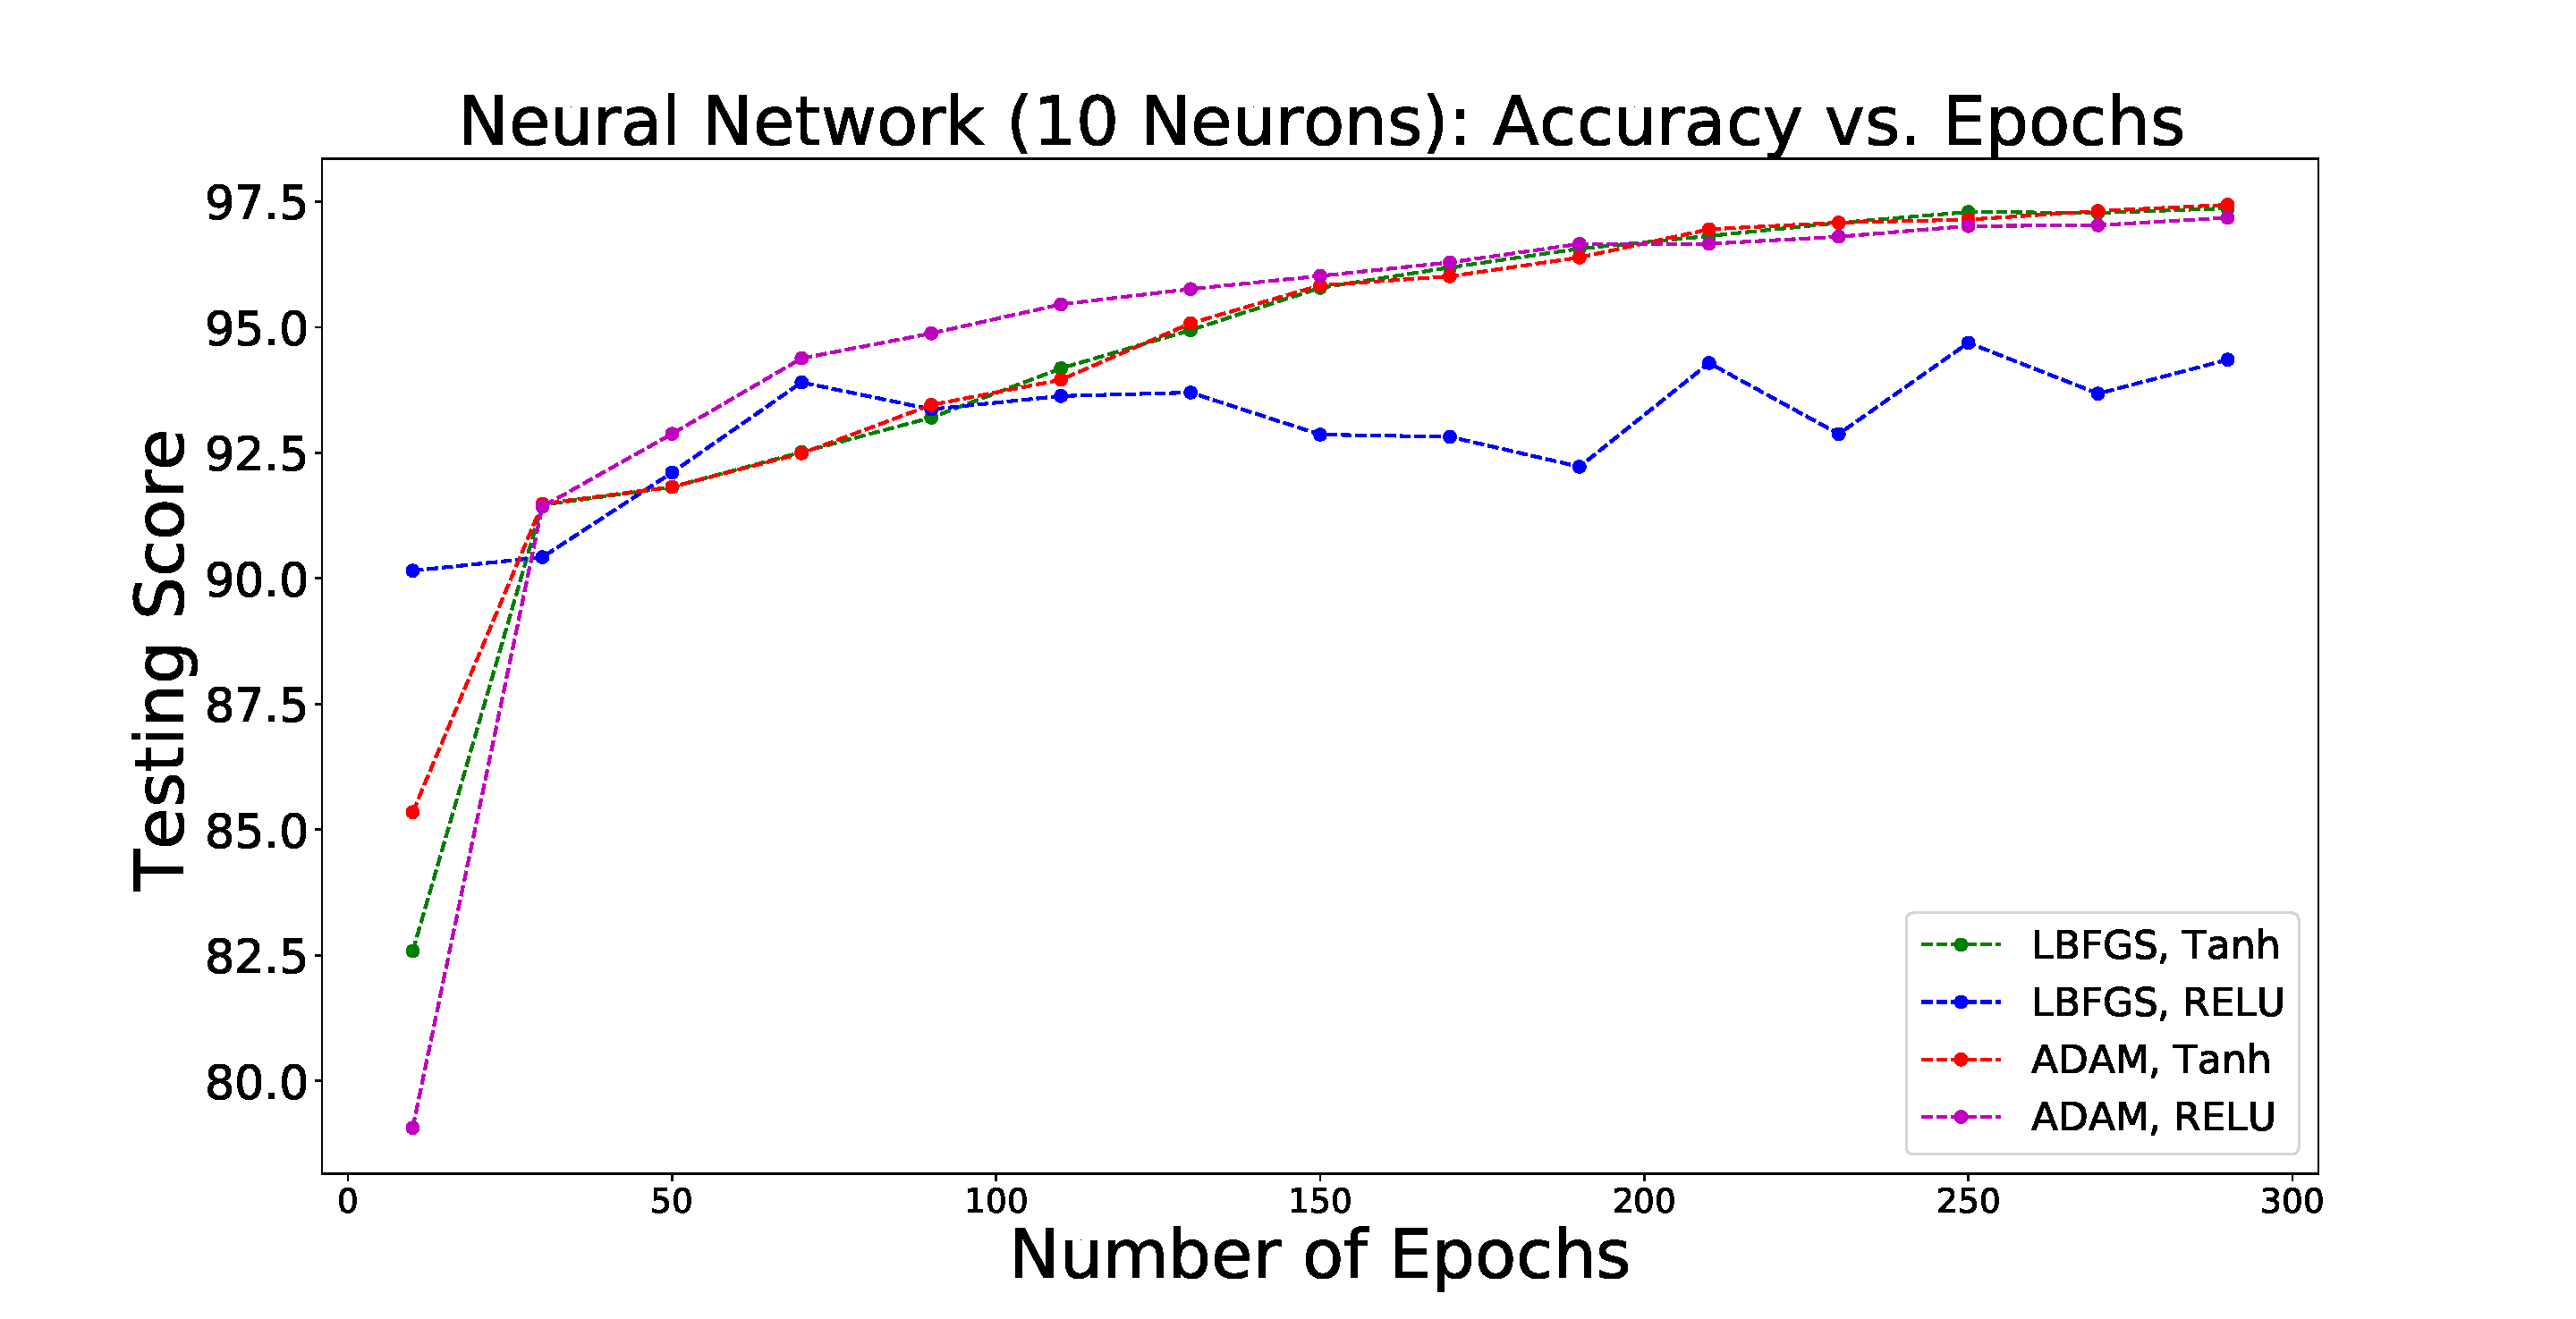
\includegraphics[width=0.5\textwidth]{plots/nn_epochs.pdf}
\caption{
Dependence on epochs for different solvers and activation function
}
\label{fig:NN_epochs}
\end{figure}

%The next step was to see the effect of multiple hidden layers and number of neurons on the accuracy. In this case we found no clear dependence, and it seems as though the network doesn't overtraiin even for a higher number of neurons. This could be explained by the less number of iterations. Higher number of hidden layers added nothing more to the accuracy and serve to only over-fit the data.\\


\begin{figure}[h]
%\centerin
\hspace*{-0.5cm}
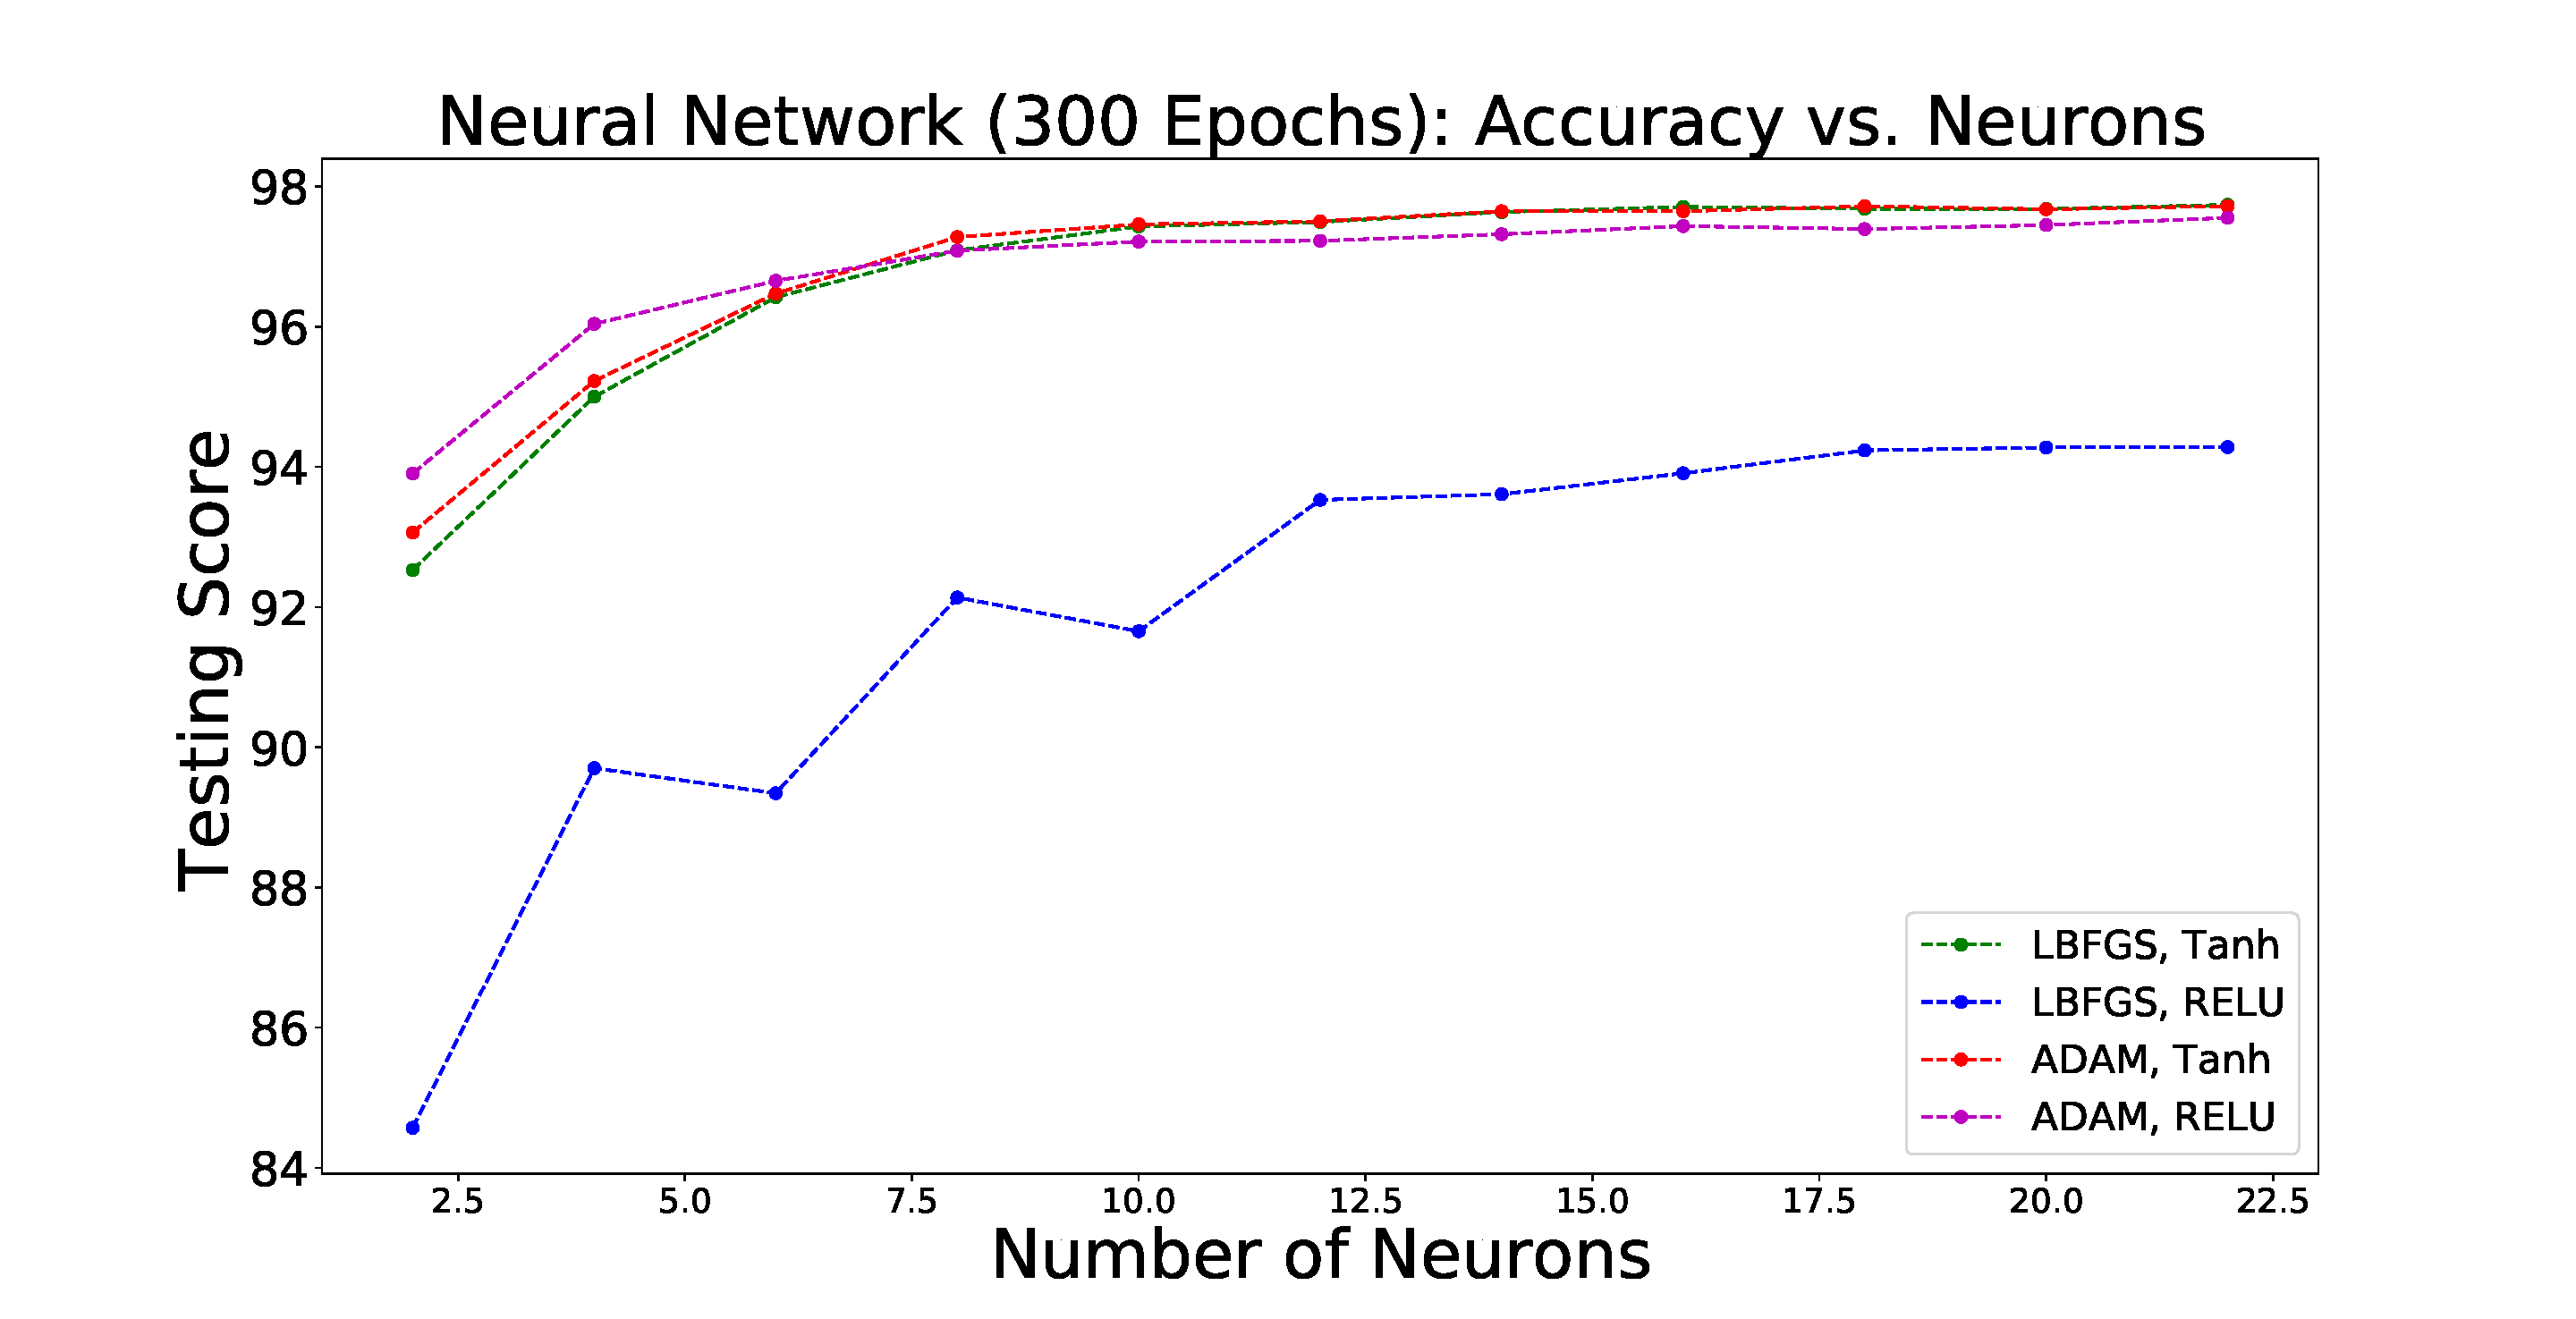
\includegraphics[width=0.5\textwidth]{plots/nn_neurons_300epochs.pdf}
%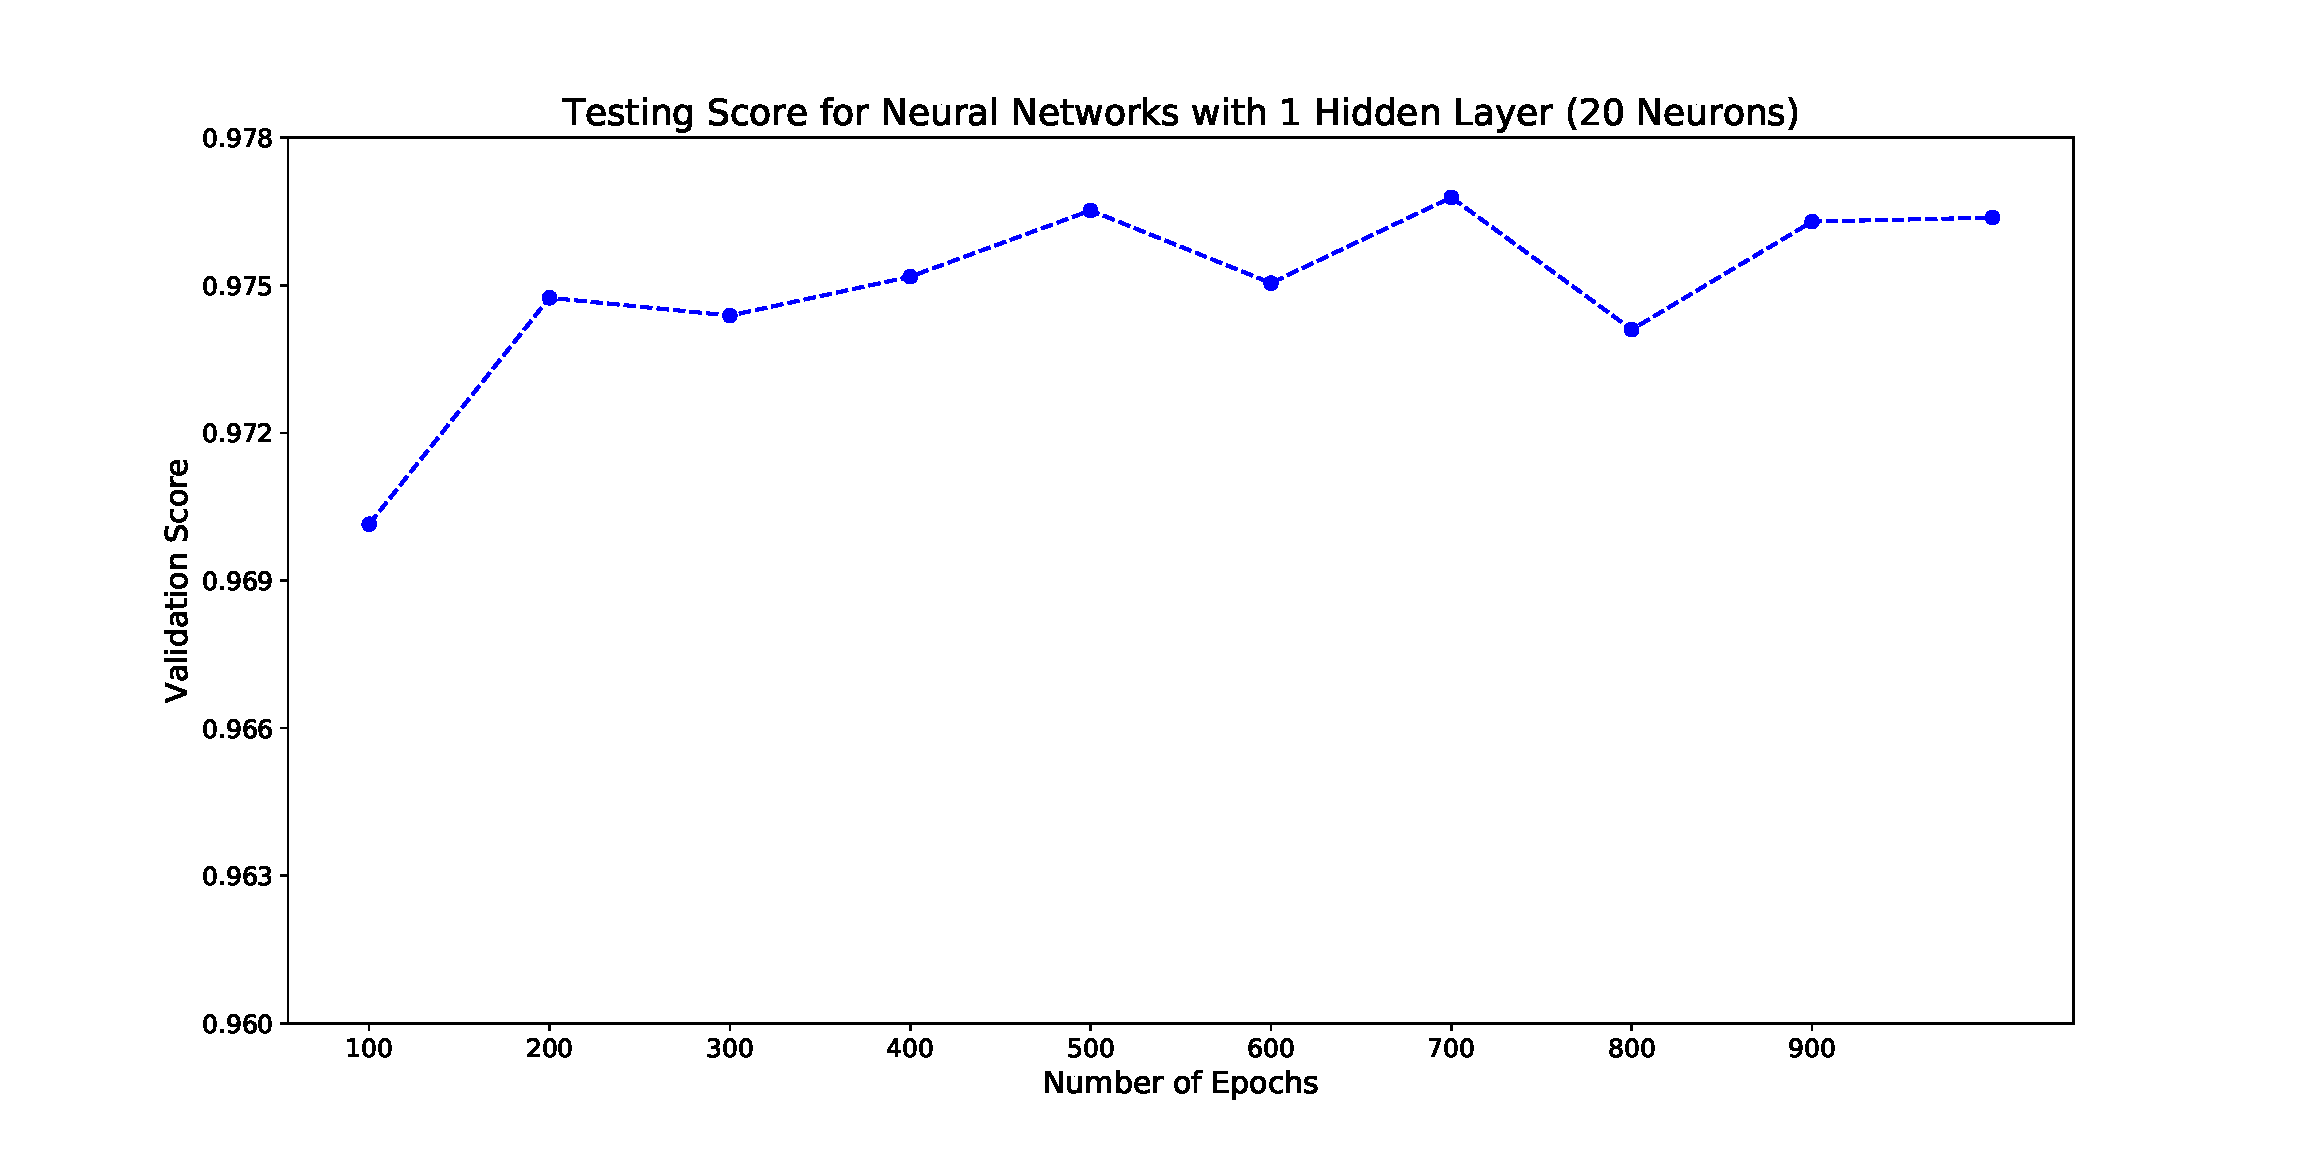
\includegraphics[width=\twopicsp\textwidth]{plots/epochsvsscore2_10seeds.pdf}
\caption{Dependence of accuracy on number of neurons for different models.}
%\dima{I'm not sure I understand where you use Tanh or RELU activations, if we have only one hidden layer with sigmoid activation (I guess) for classification?}}
\label{fig:NN_neurons}
\end{figure}

Domains for NN with only two input features are shown in Figure \ref{fig:NN_domains}.
%\dima{As above, I don't think it makes sense to use more than 2 nodes in the hidden layer here, since there are only two input features.}


\begin{figure}[h]
%\centerin
\hspace*{-1.5cm}
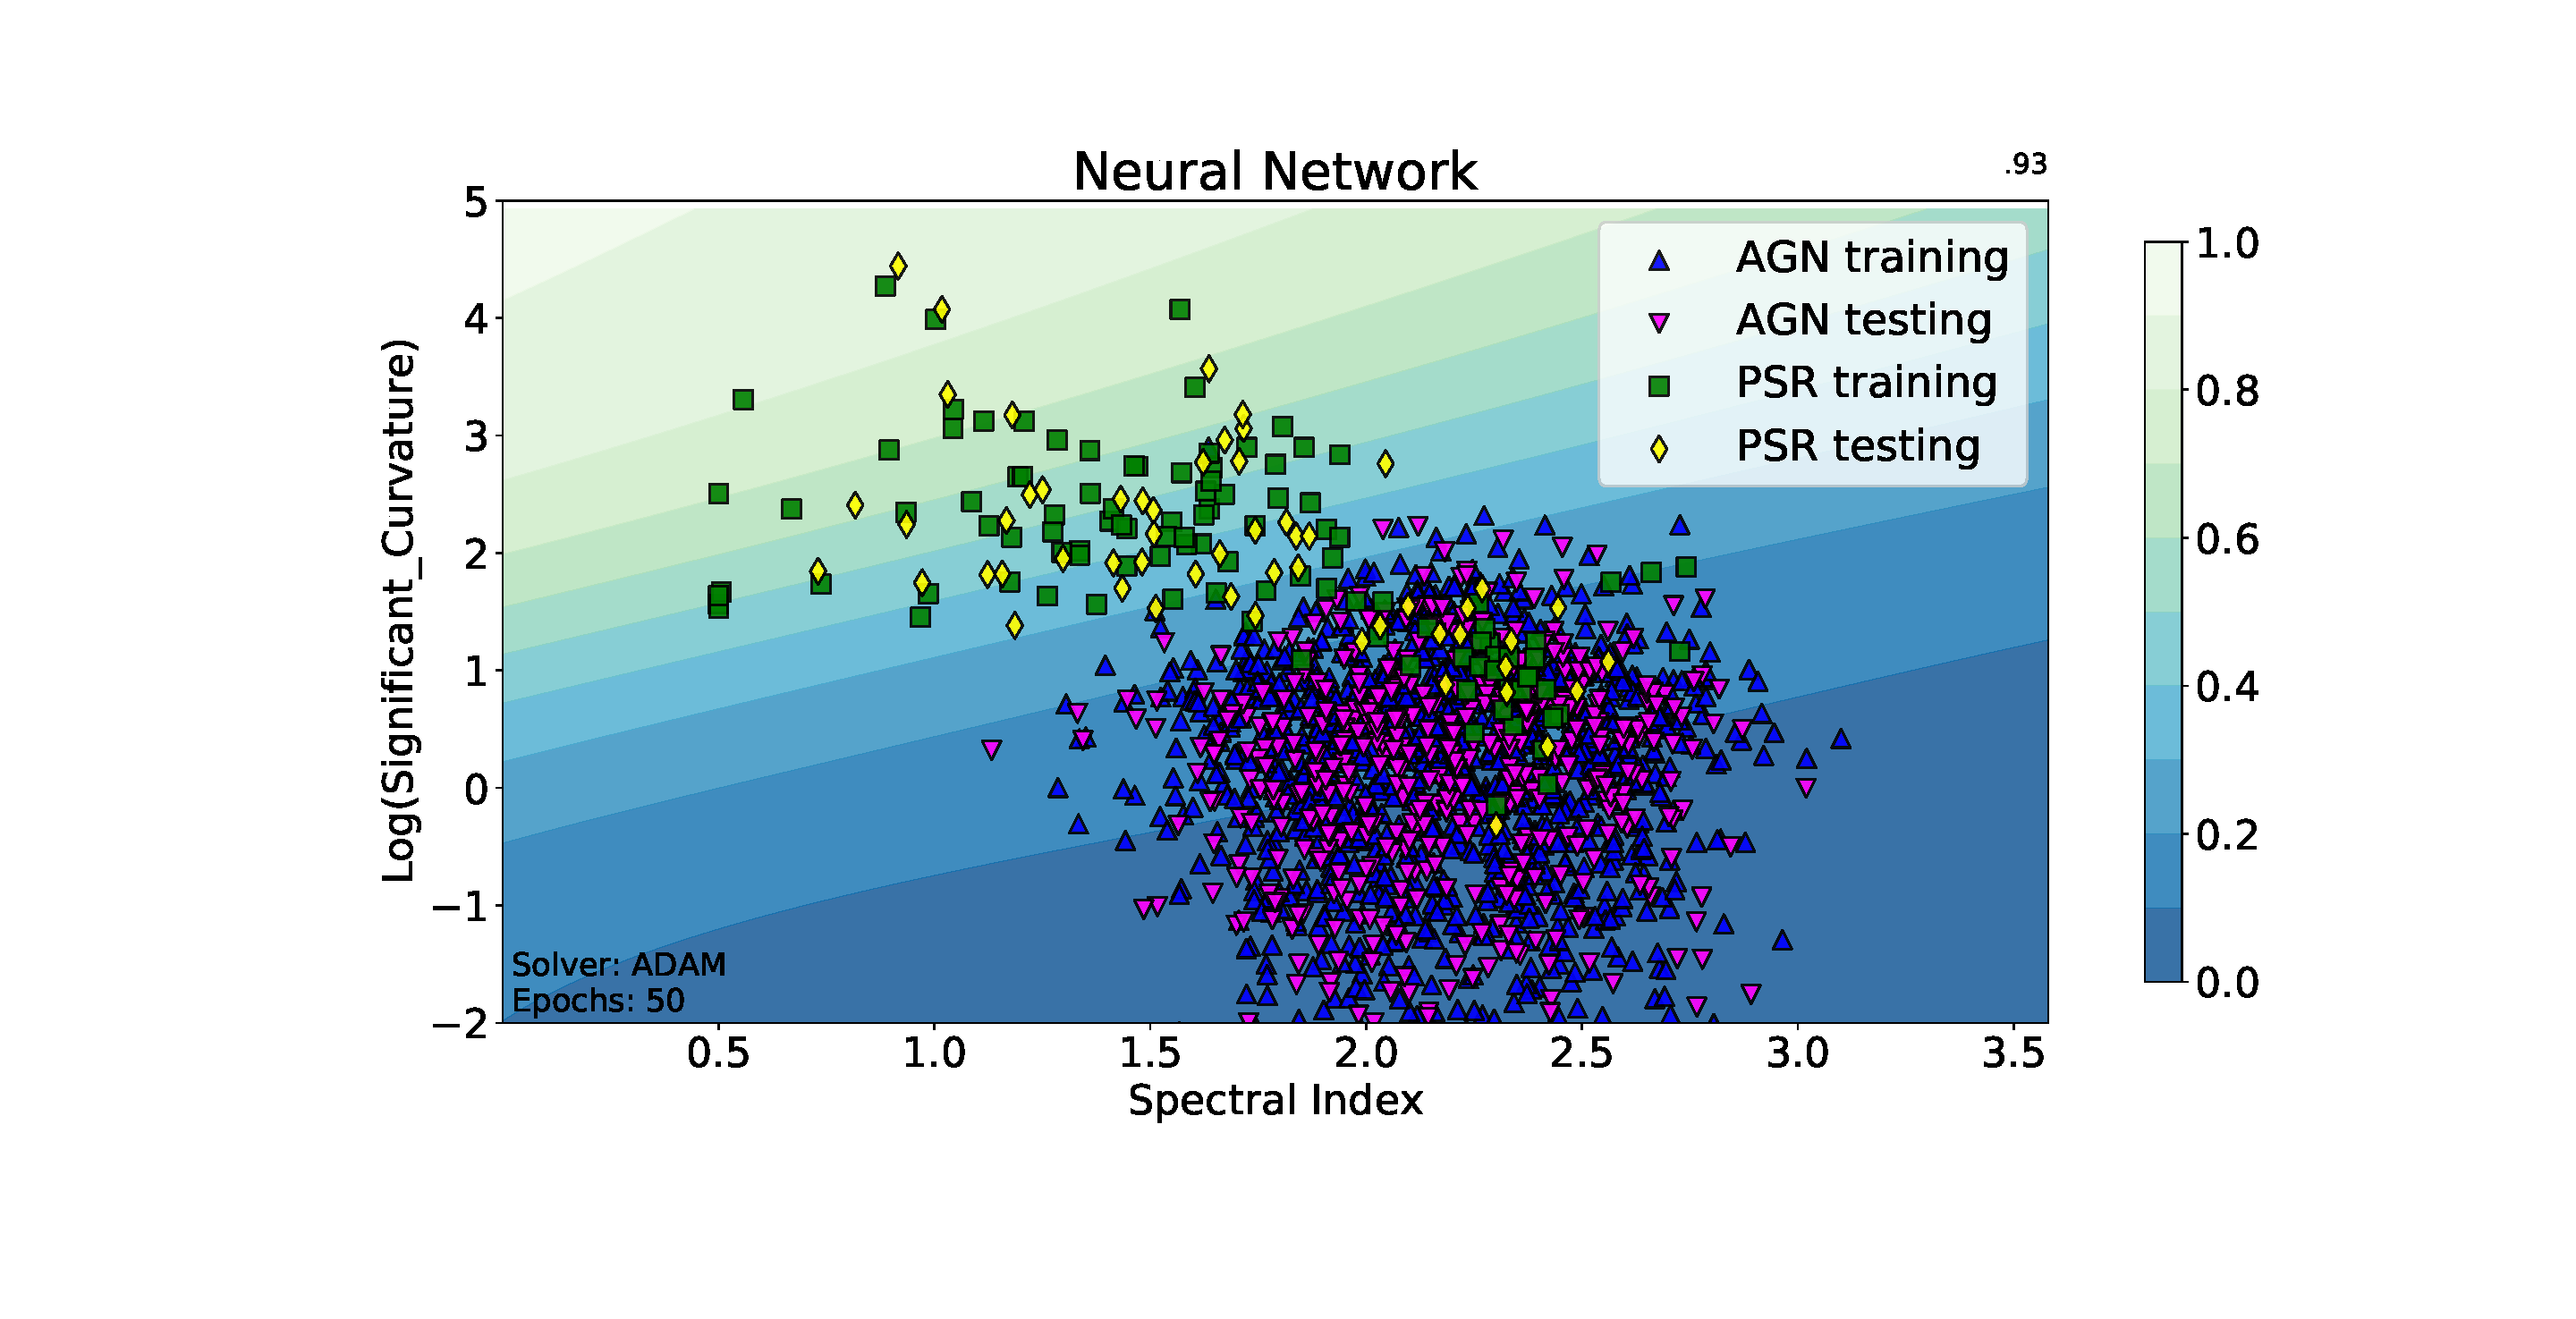
\includegraphics[width=0.6\textwidth]{plots/classification_domains/nn_adam_10_tanh_50_final.pdf}
\hspace*{-1.5cm}
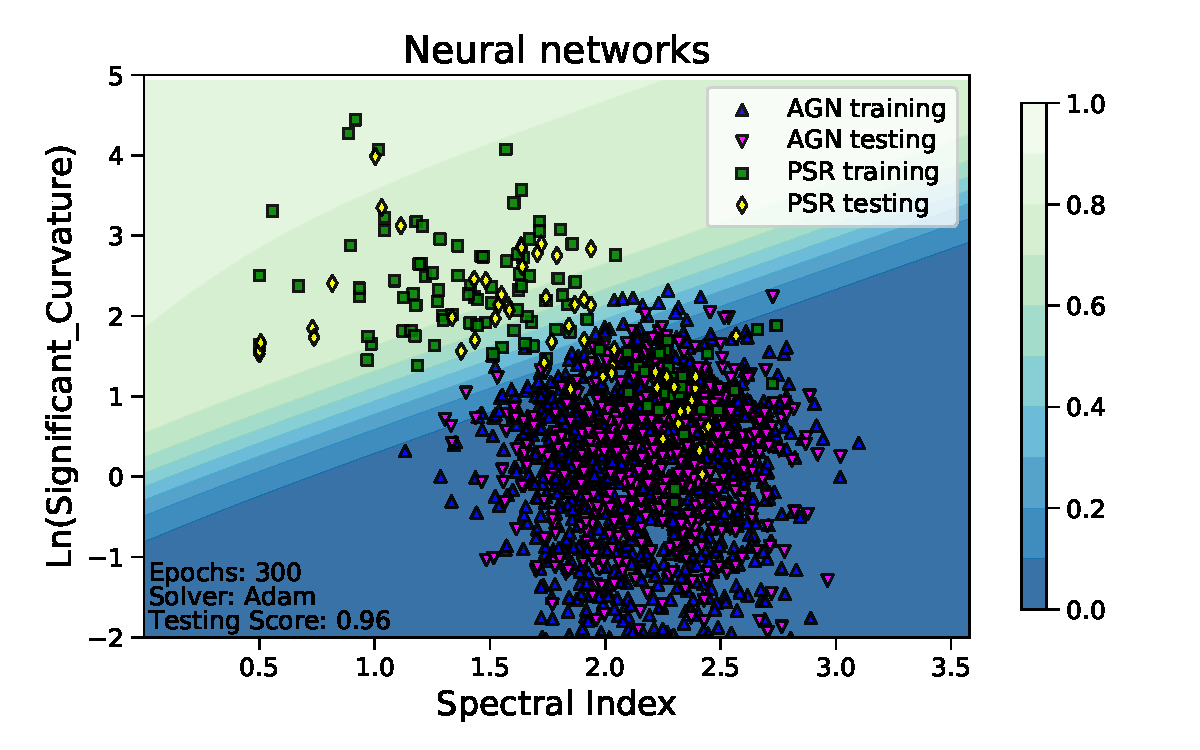
\includegraphics[width=0.6\textwidth]{plots/classification_domains/nn_adam_10_tanh_300_final.pdf}
\caption{Classification Domains for Neural Networks for the same complexity of 2 Neurons and tanh activation, using ADAM solver. }
\label{fig:NN_domains}
\end{figure}

\subsection{Boosted Decision Trees}

The free parameters for BDT algorithms are similar to RF algorithms: the number of trees and the maximal depth.
We will use the gradient boosting algorithm for the construction of BDT.
The classification is performed by a weighted average of trees, where the trees are constructed recursively in order to better address 
misclassifications from the previous step. The new trees are added with an additional parameter $\nu$ called learning rate.
We will use learning rate $\nu = 0.3$.
\dima{I'm not sure we need to discuss the learning rate, since we haven't done so in, e.g., neural networks}
Dependence of the accuracy on tree depth is shown in Figure \ref{fig:BDT_depth}. The plot shows that depth of 2 and 100 trees is near the optimal limit. 
%\dima{Which depth do we use for the final algorithm, it looks like depth 2 gives the best results. What about depth = 1?}

\begin{figure}[h]
%\centerin
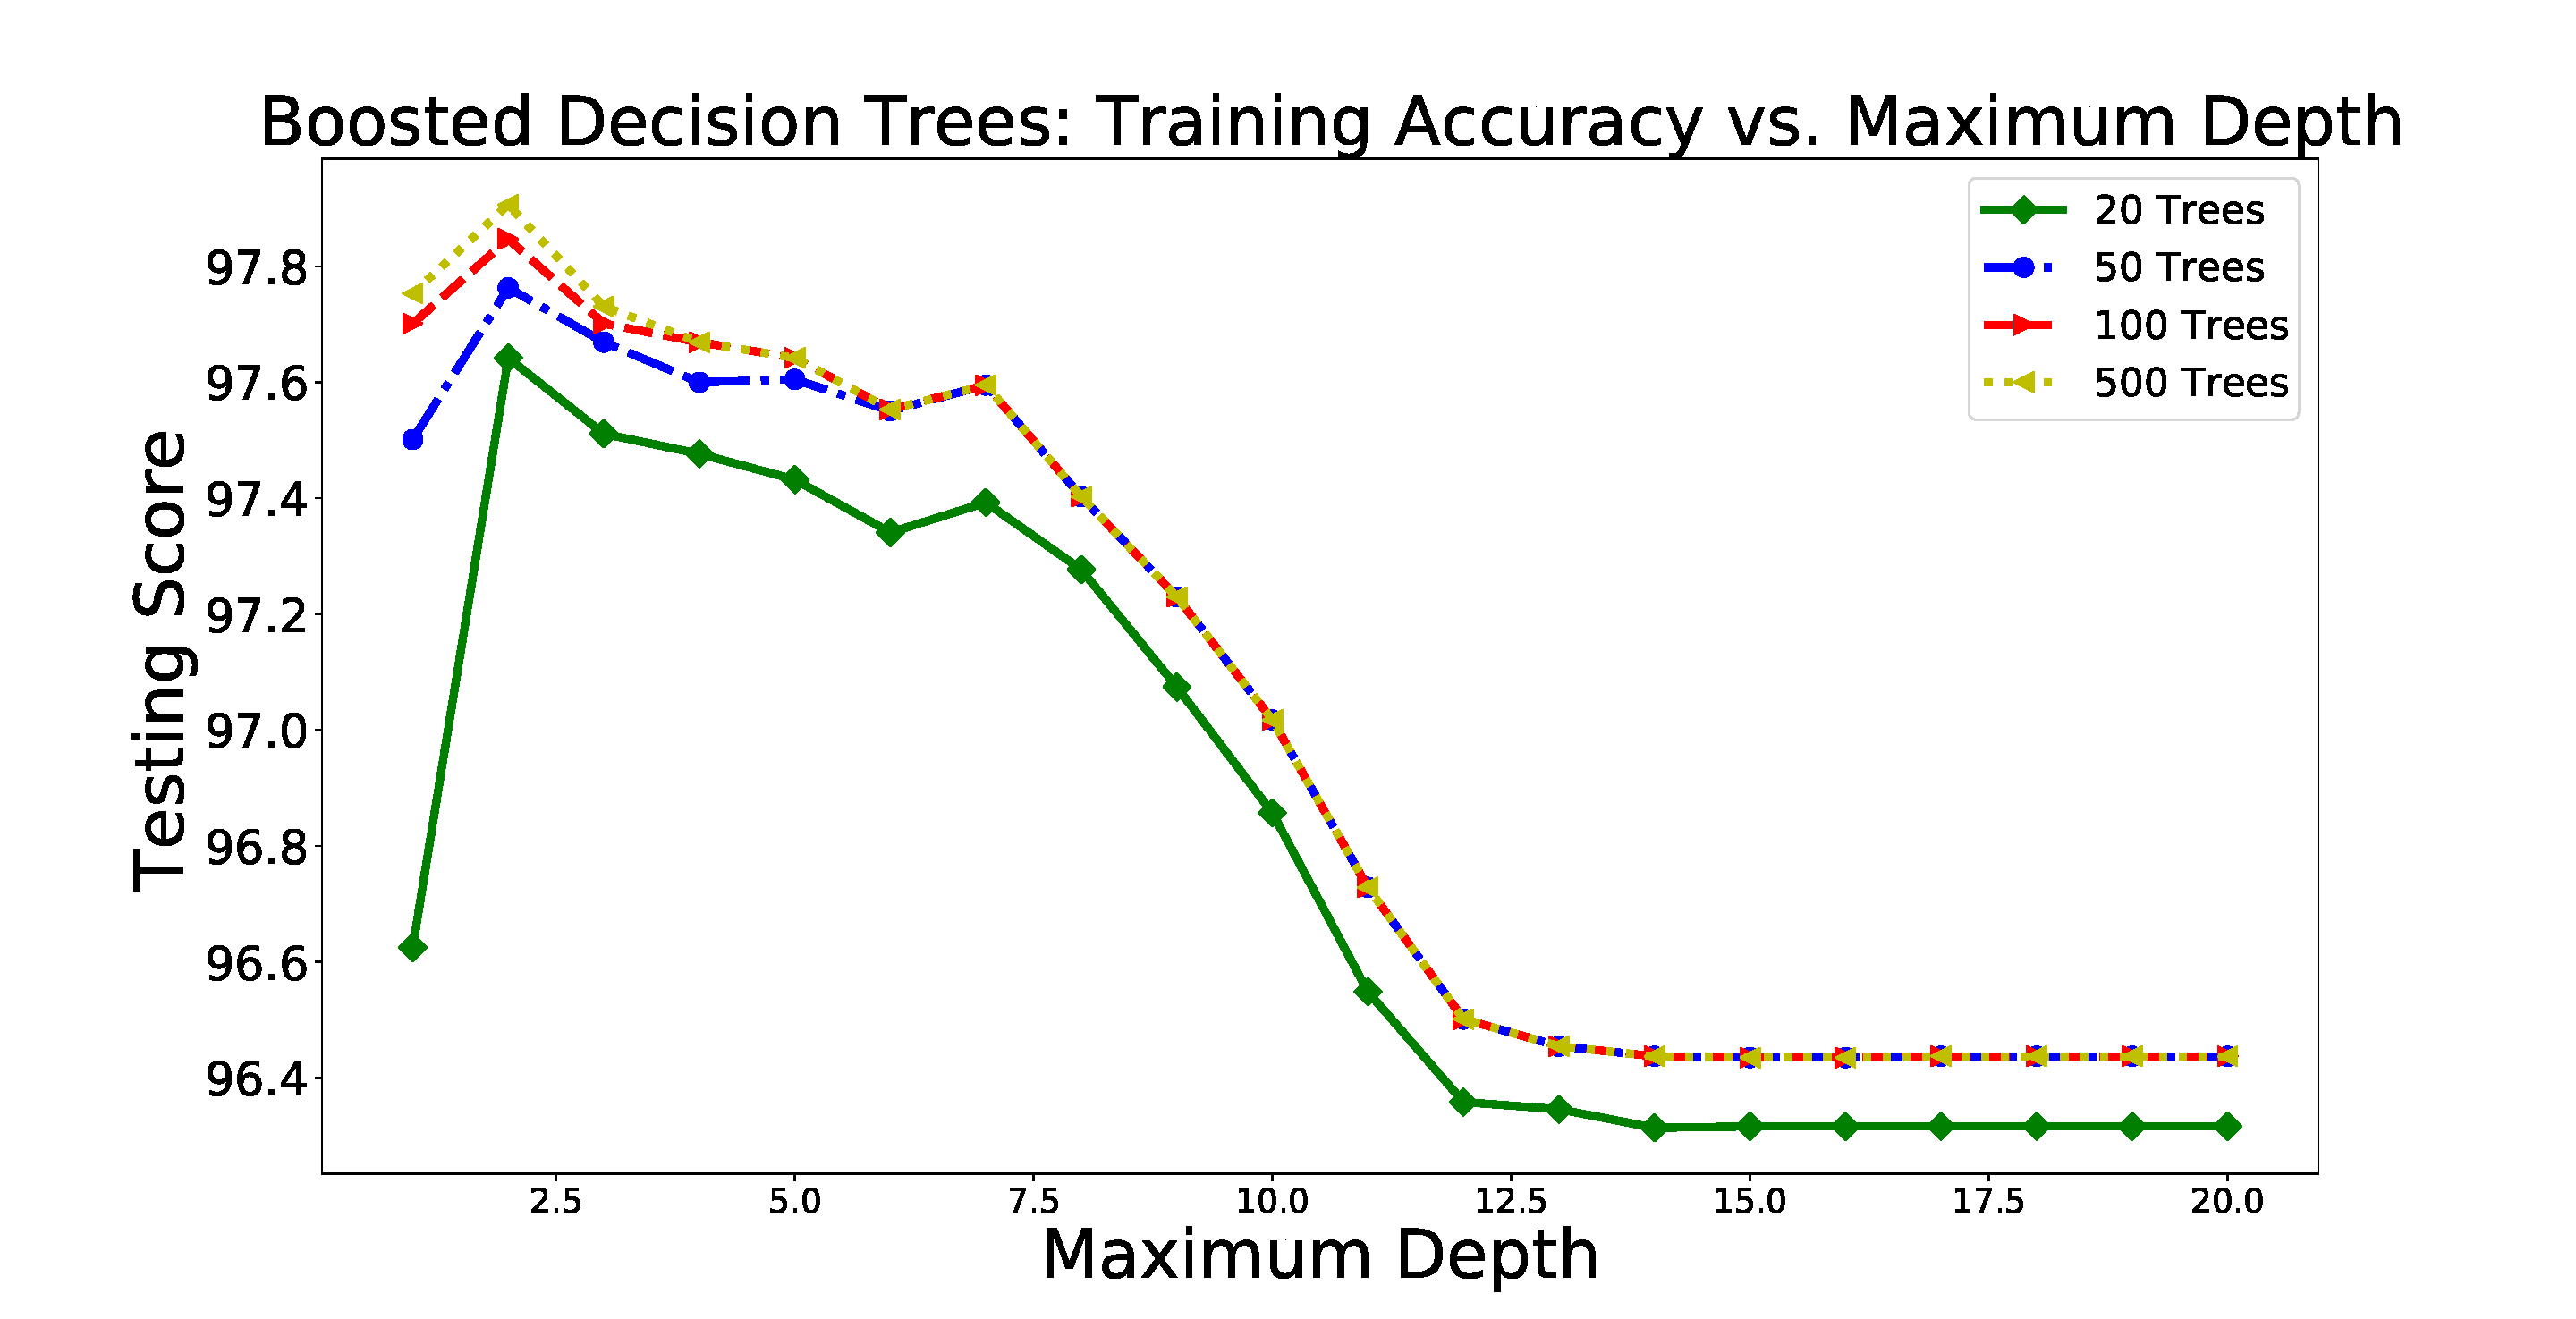
\includegraphics[width=\twopicsp\textwidth]{plots/bdt_train.pdf}
%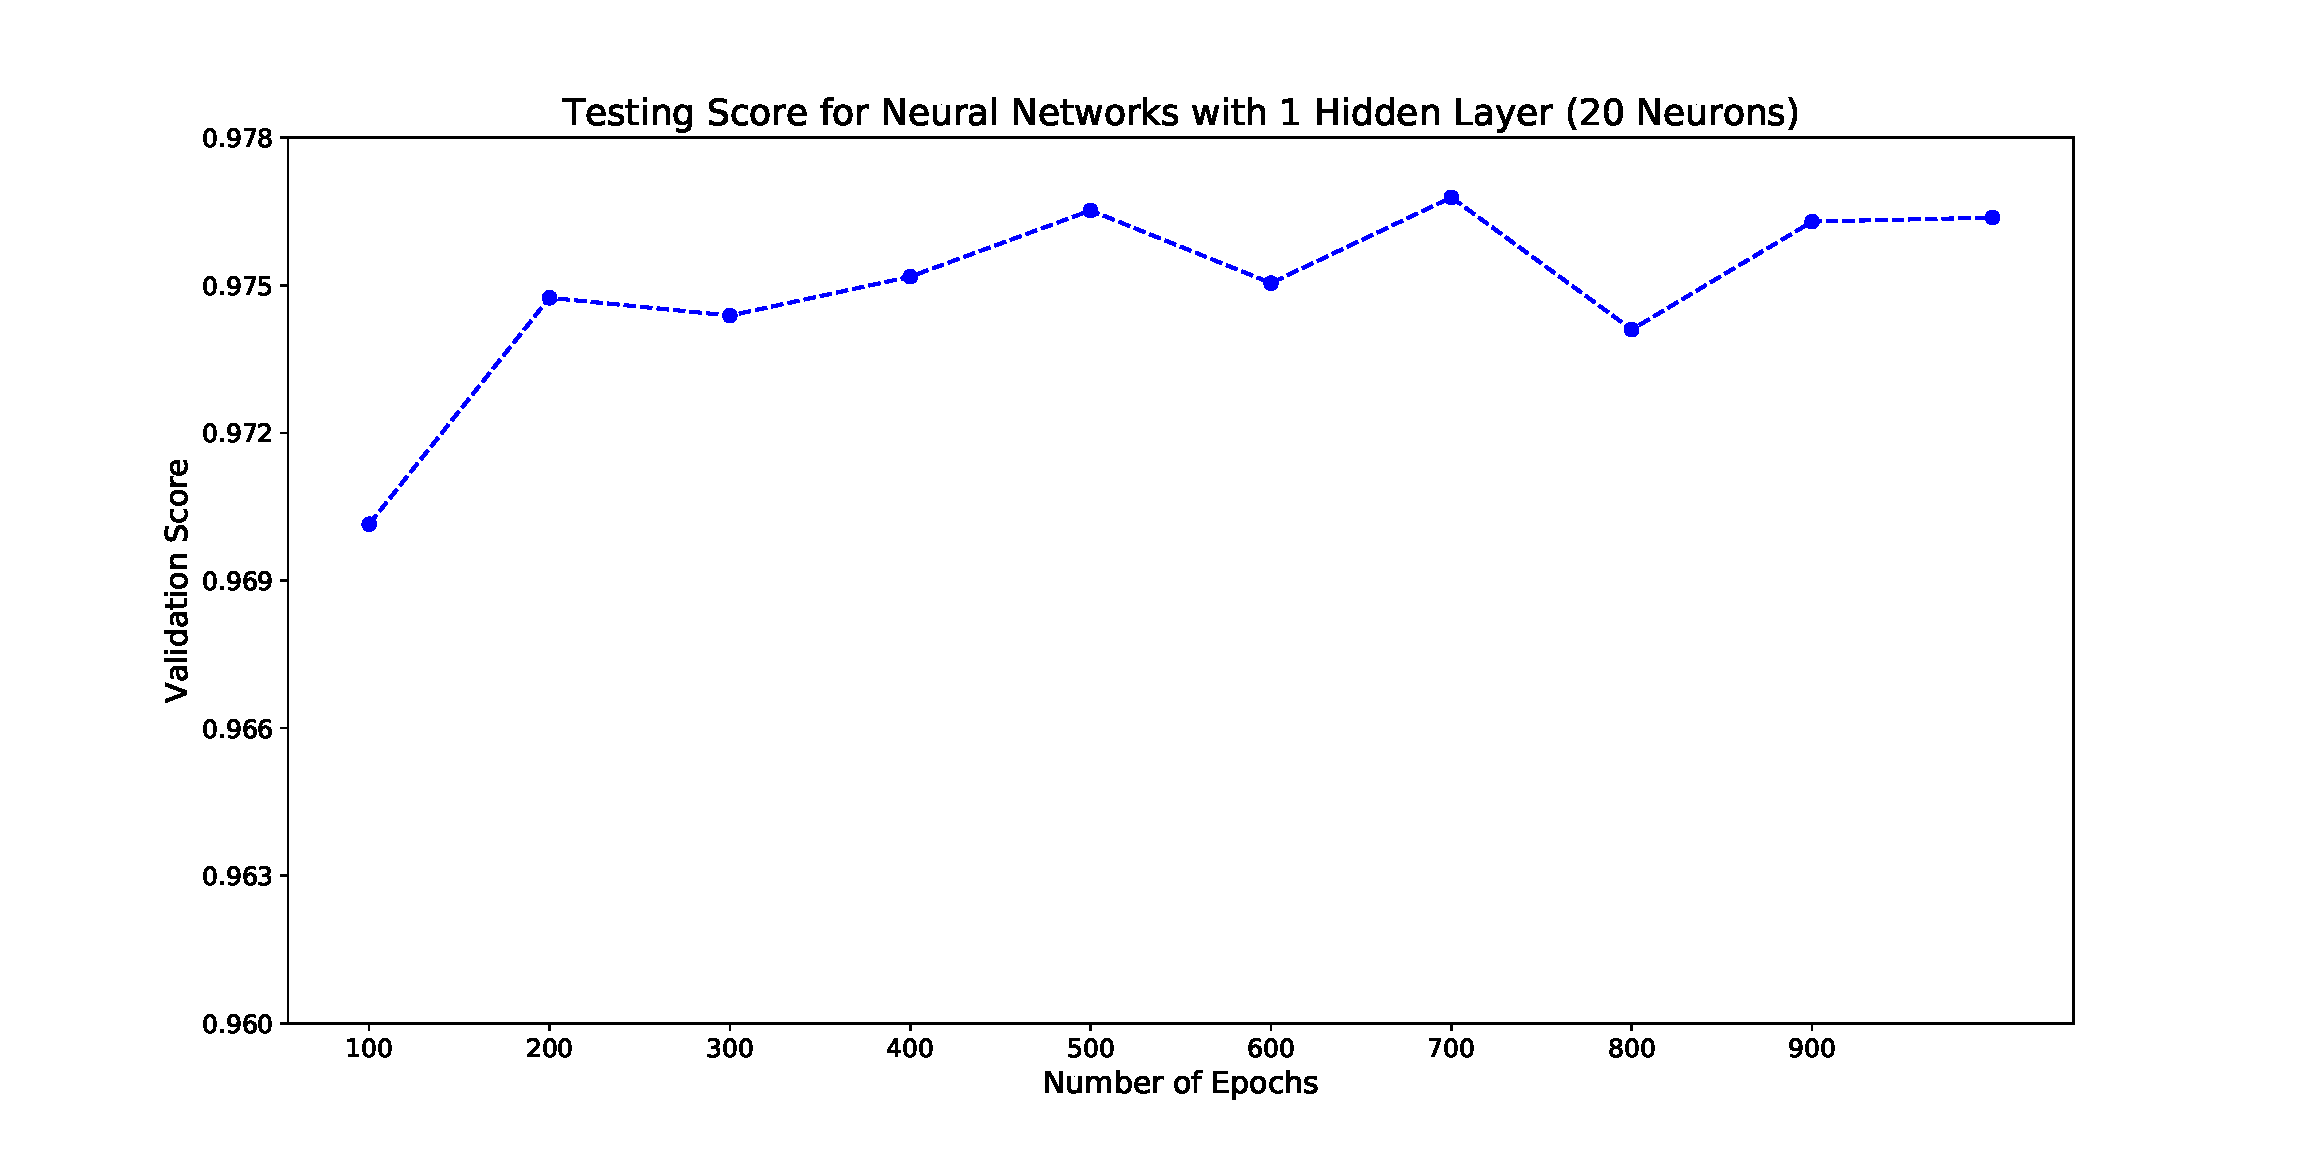
\includegraphics[width=\twopicsp\textwidth]{plots/epochsvsscore2_10seeds.pdf}
\caption{Dependence of BDT accuracy on maximum depth}
\label{fig:BDT_depth}
\end{figure}

The Classification domains in case of two features for the maximal depth of 3 and 15 is presented in Figure \ref{fig:BDT_domains}. The greater than a percent decrease in the accuracy from a max depth of 3 to a max depth of 15 can be explained by the domains, where we see a pattern of almost over-fitting the data. While for 2 features the decrease is small, it should increase as we increase the number of features, with a lower complexity network being enough for a good accuracy.
%Boosted Decision Trees again show a similar effect as Random forests in their classification, and have a significant difference when the model complexity is changed.

\begin{figure}[h]
%\centerin
\hspace*{-1.5cm}
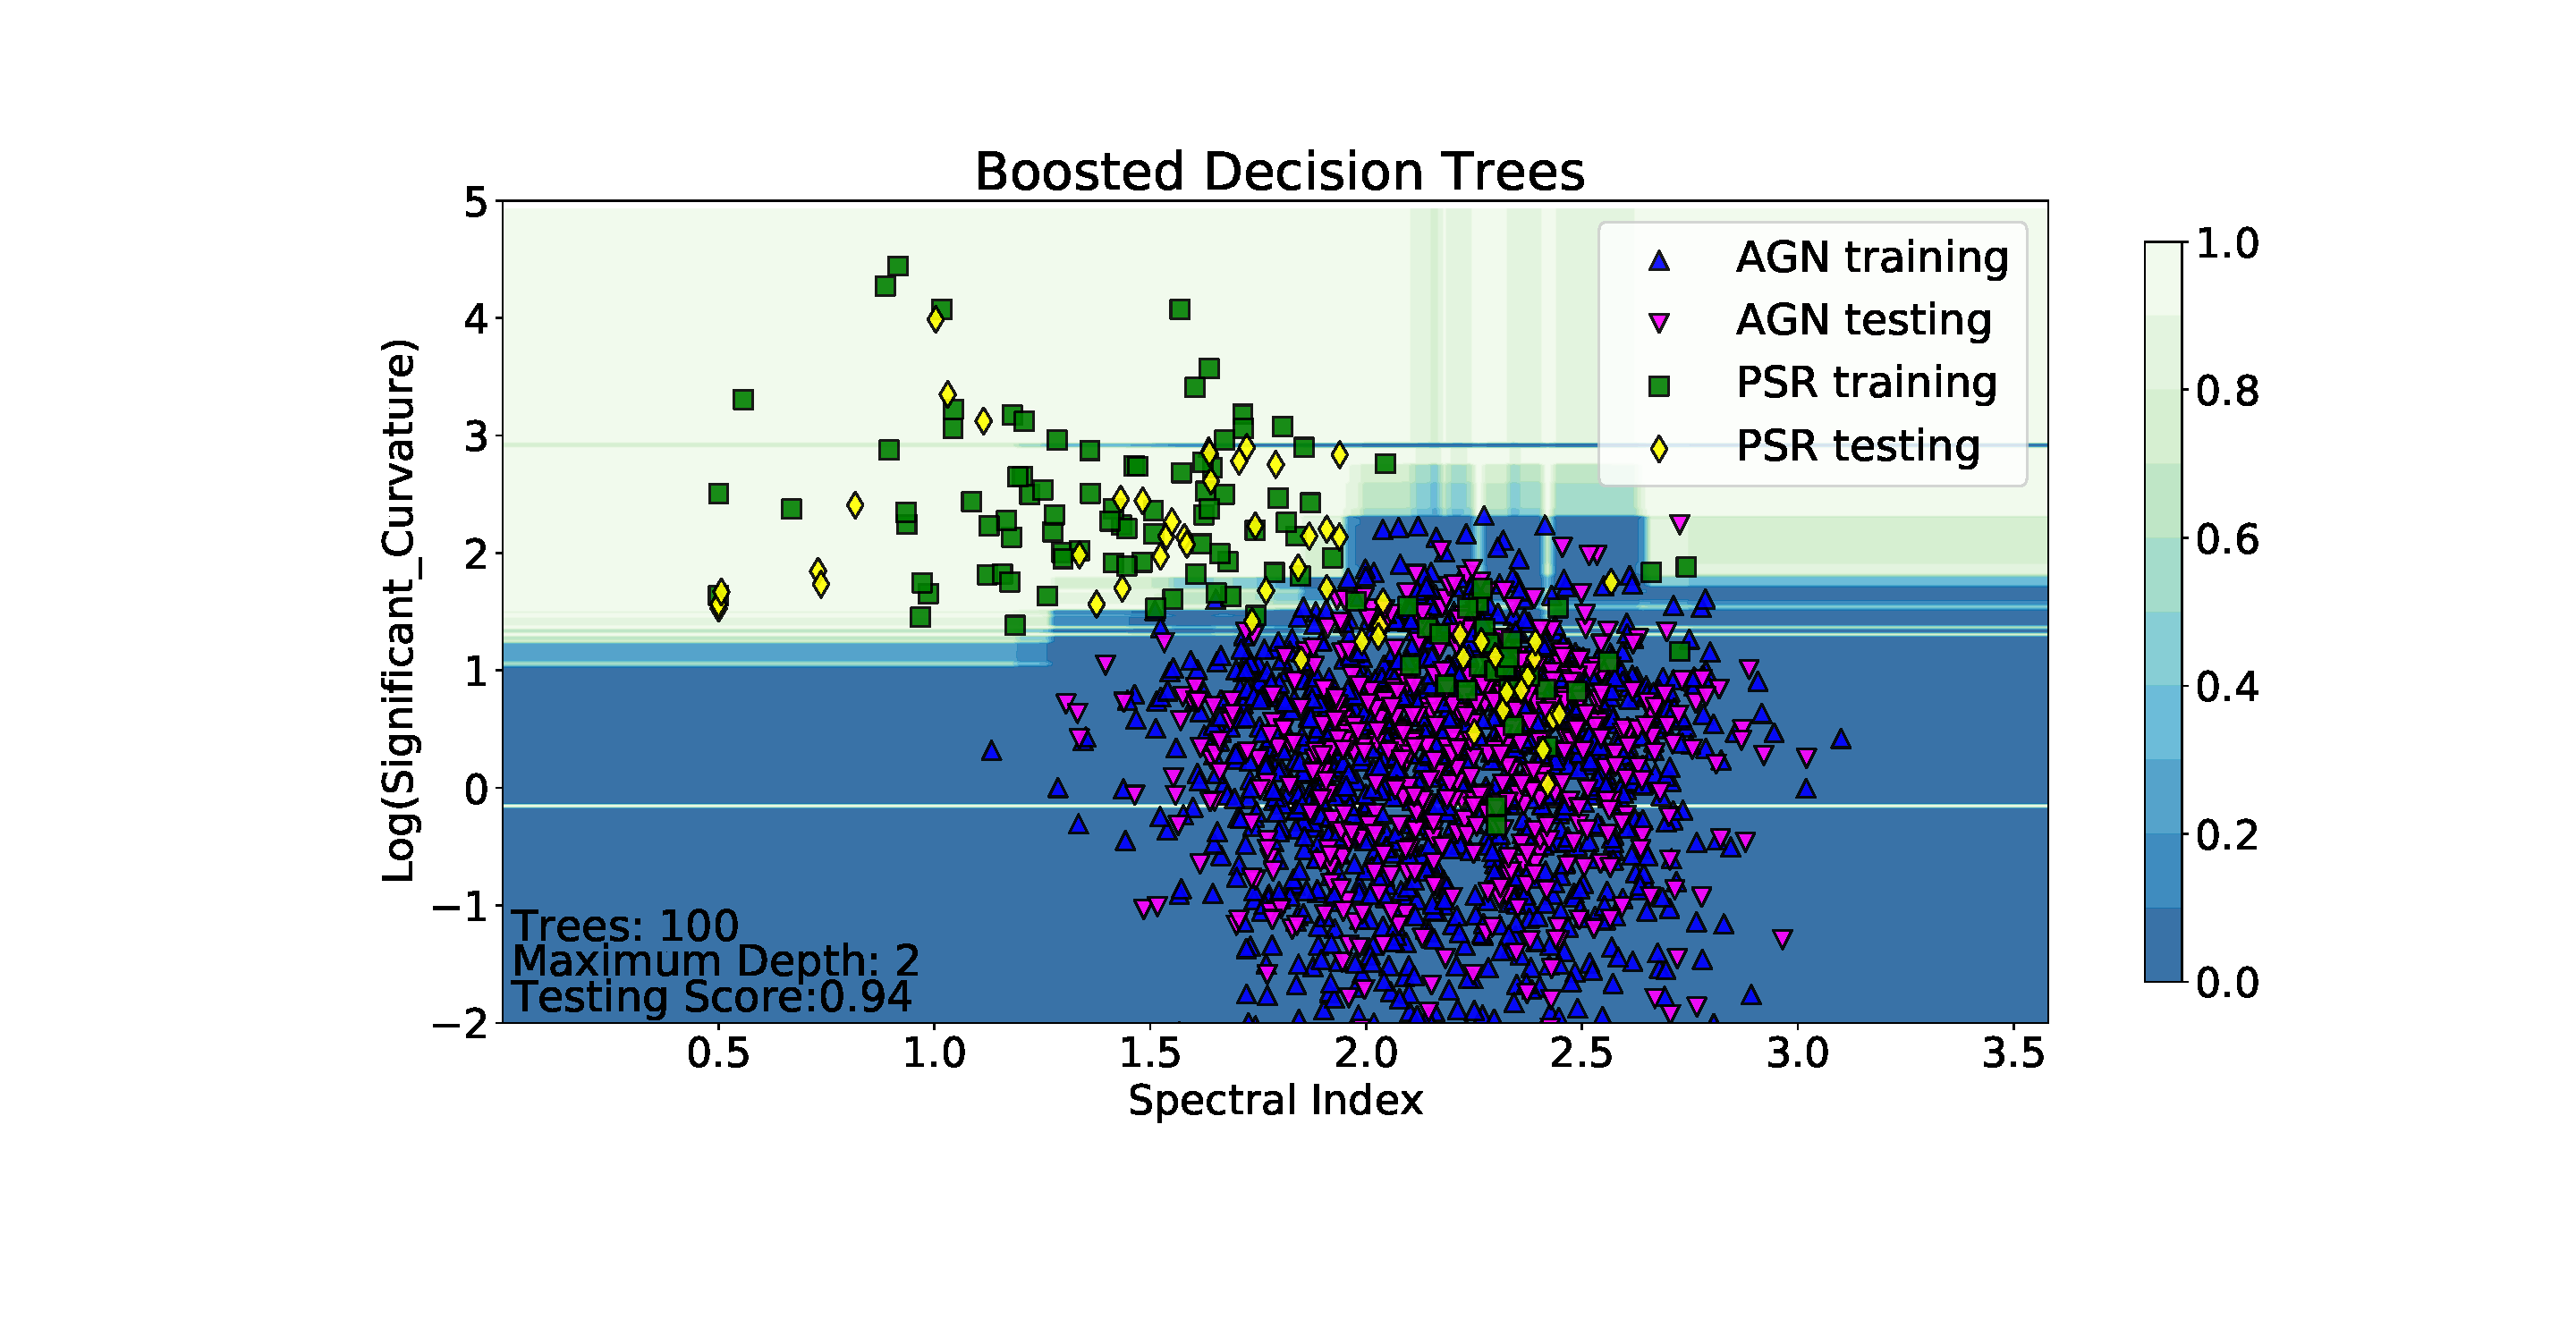
\includegraphics[width=0.6\textwidth]{plots/classification_domains/bdt_100_2.pdf}
\hspace*{-1.5cm}
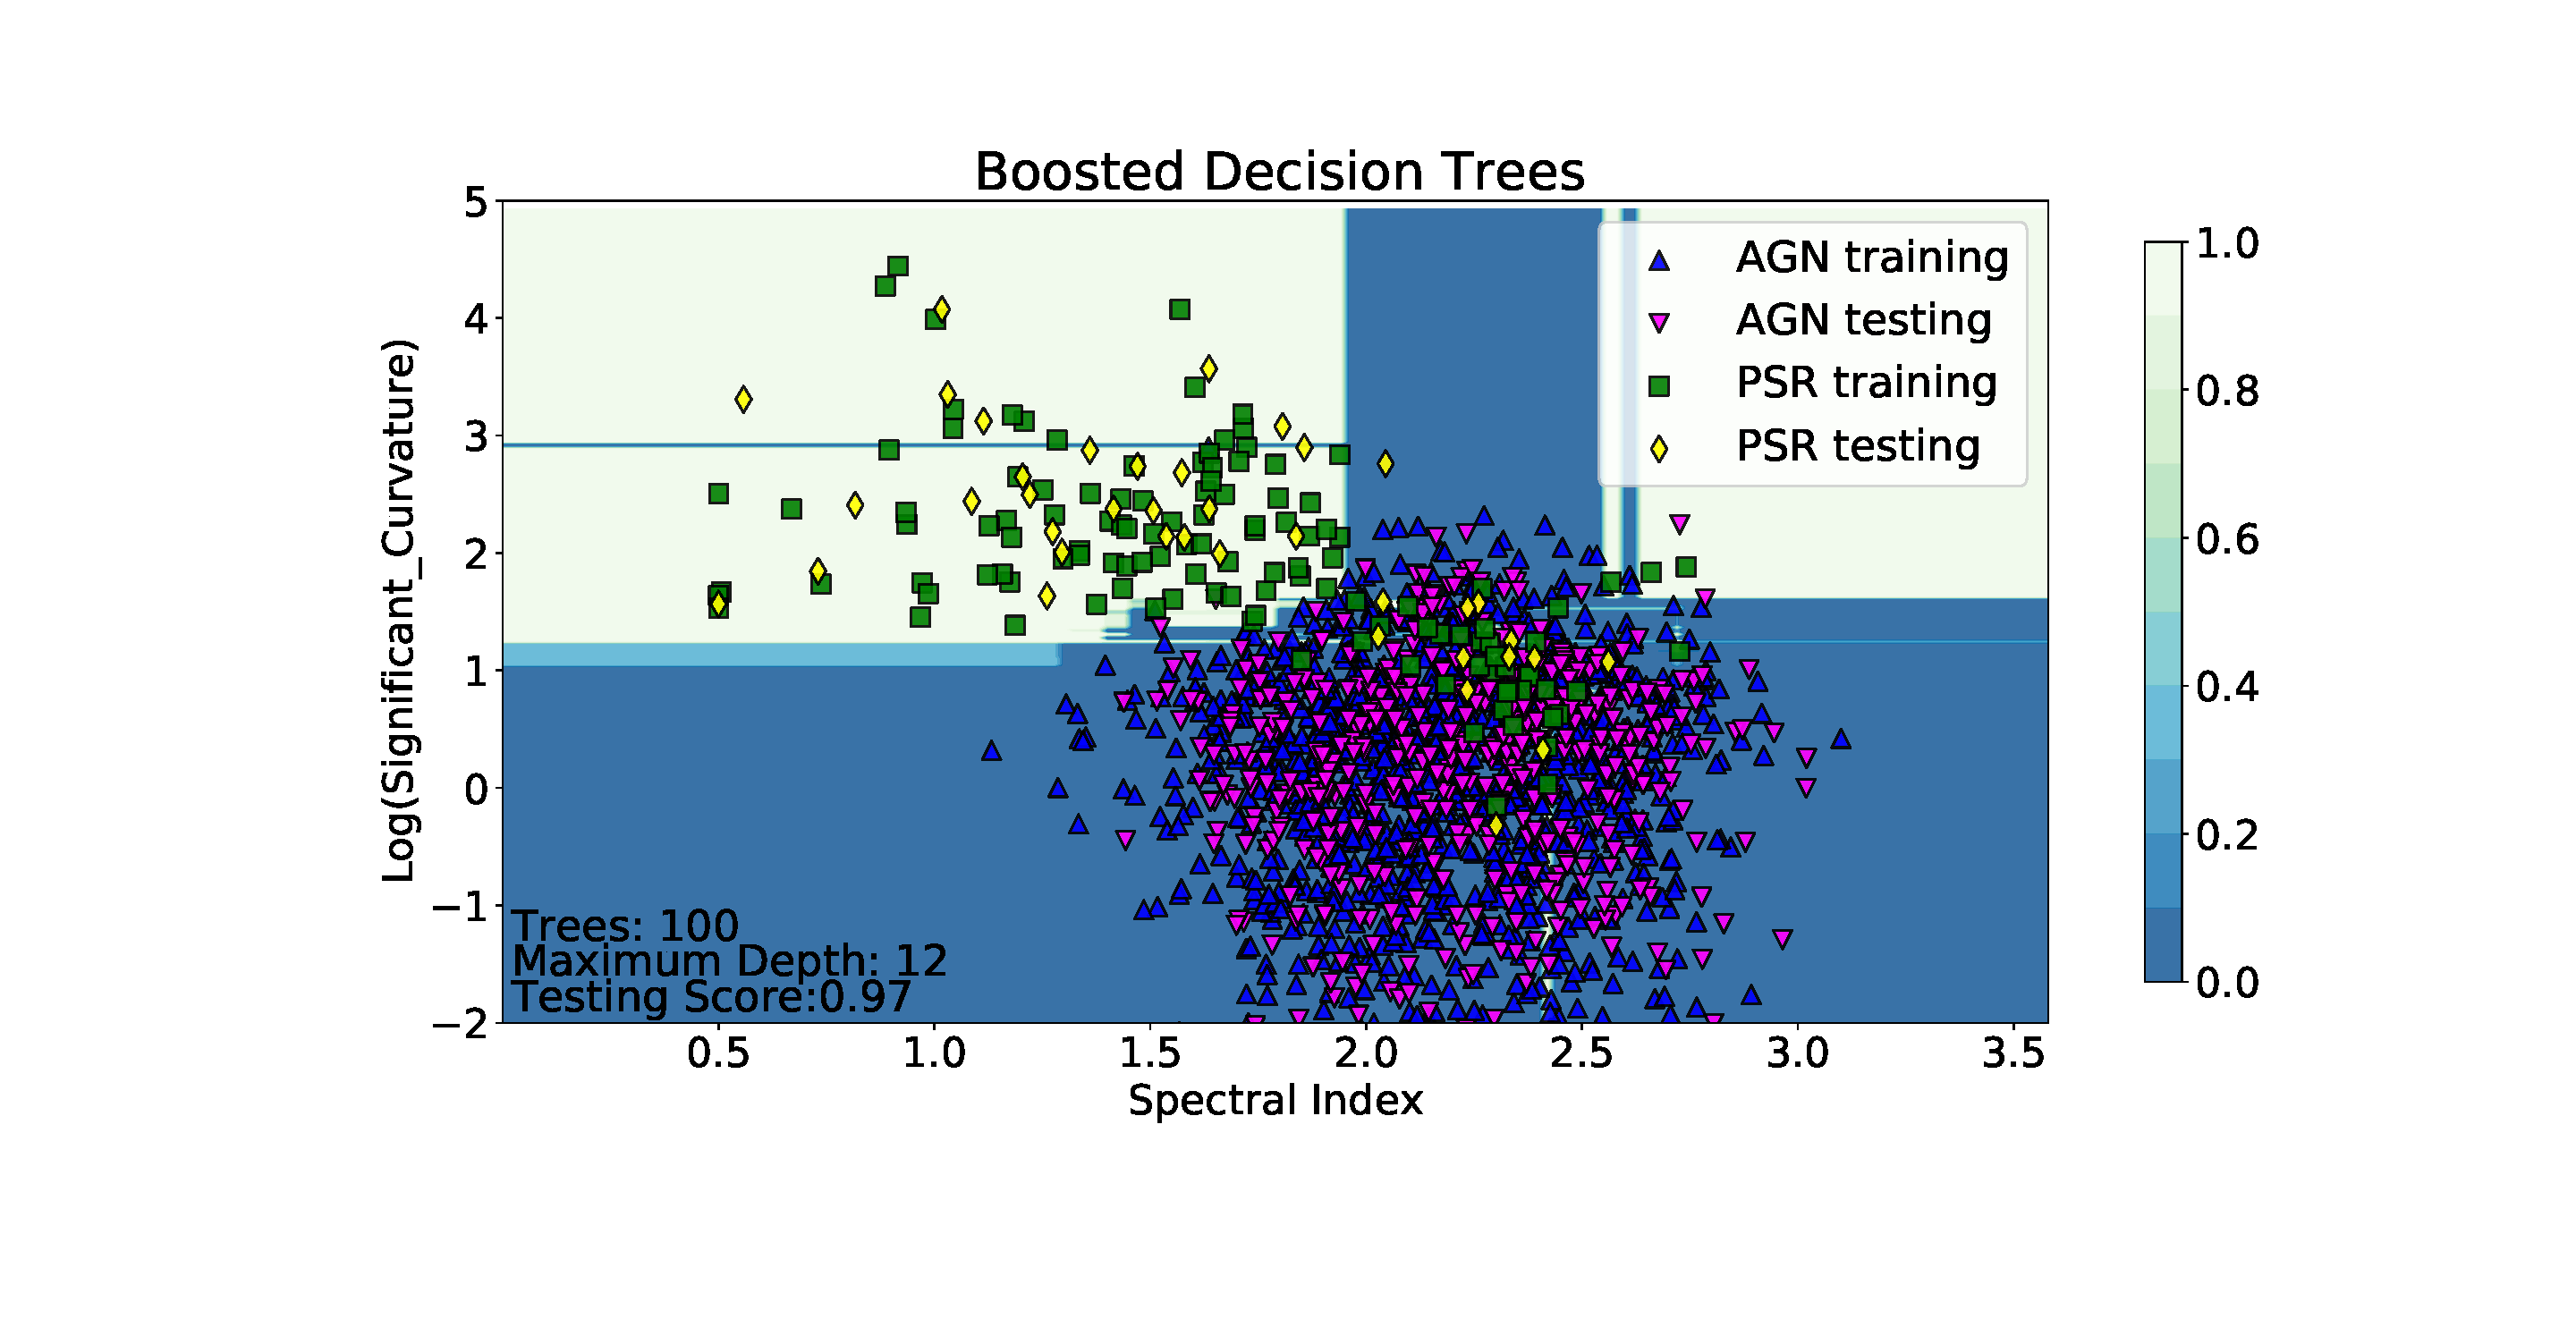
\includegraphics[width=0.6\textwidth]{plots/classification_domains/bdt_100_12.pdf}
\caption{Classification Domains for BDT}
\label{fig:BDT_domains}
\end{figure}


\begin{comment}
Is learning rate equivalent to the 
Boosted Decision Trees or Gradient boosting algorithms are similar to Random Forests, having number of trees and maximum depth as parameters. However, here we also have the learning rate which specifies how fast (or slow) a model learns. This parameter is quite important, as a high value will converge faster but under-fit, whereas a lower value will over-fit. Therefore, we first chose an architecture of (50,6) and (20,6) to look at the dependence on number of trees. Here we found that low learning rate is preferred, and the maximum accuracy is reached at around 0.1-0.3. After a maximum the accuracy falls drastically since the BDT doesn't have enough time to learn properly. However, after a certain maximum depth, this doesn't hold true anymore irrespective of the number of trees. In this case, the BDT is complex enough that it learns fast and the accuracy doesn't fall even for higher learning rates. The figures below illustrate this.\\



\begin{figure}[h]
%\centerin
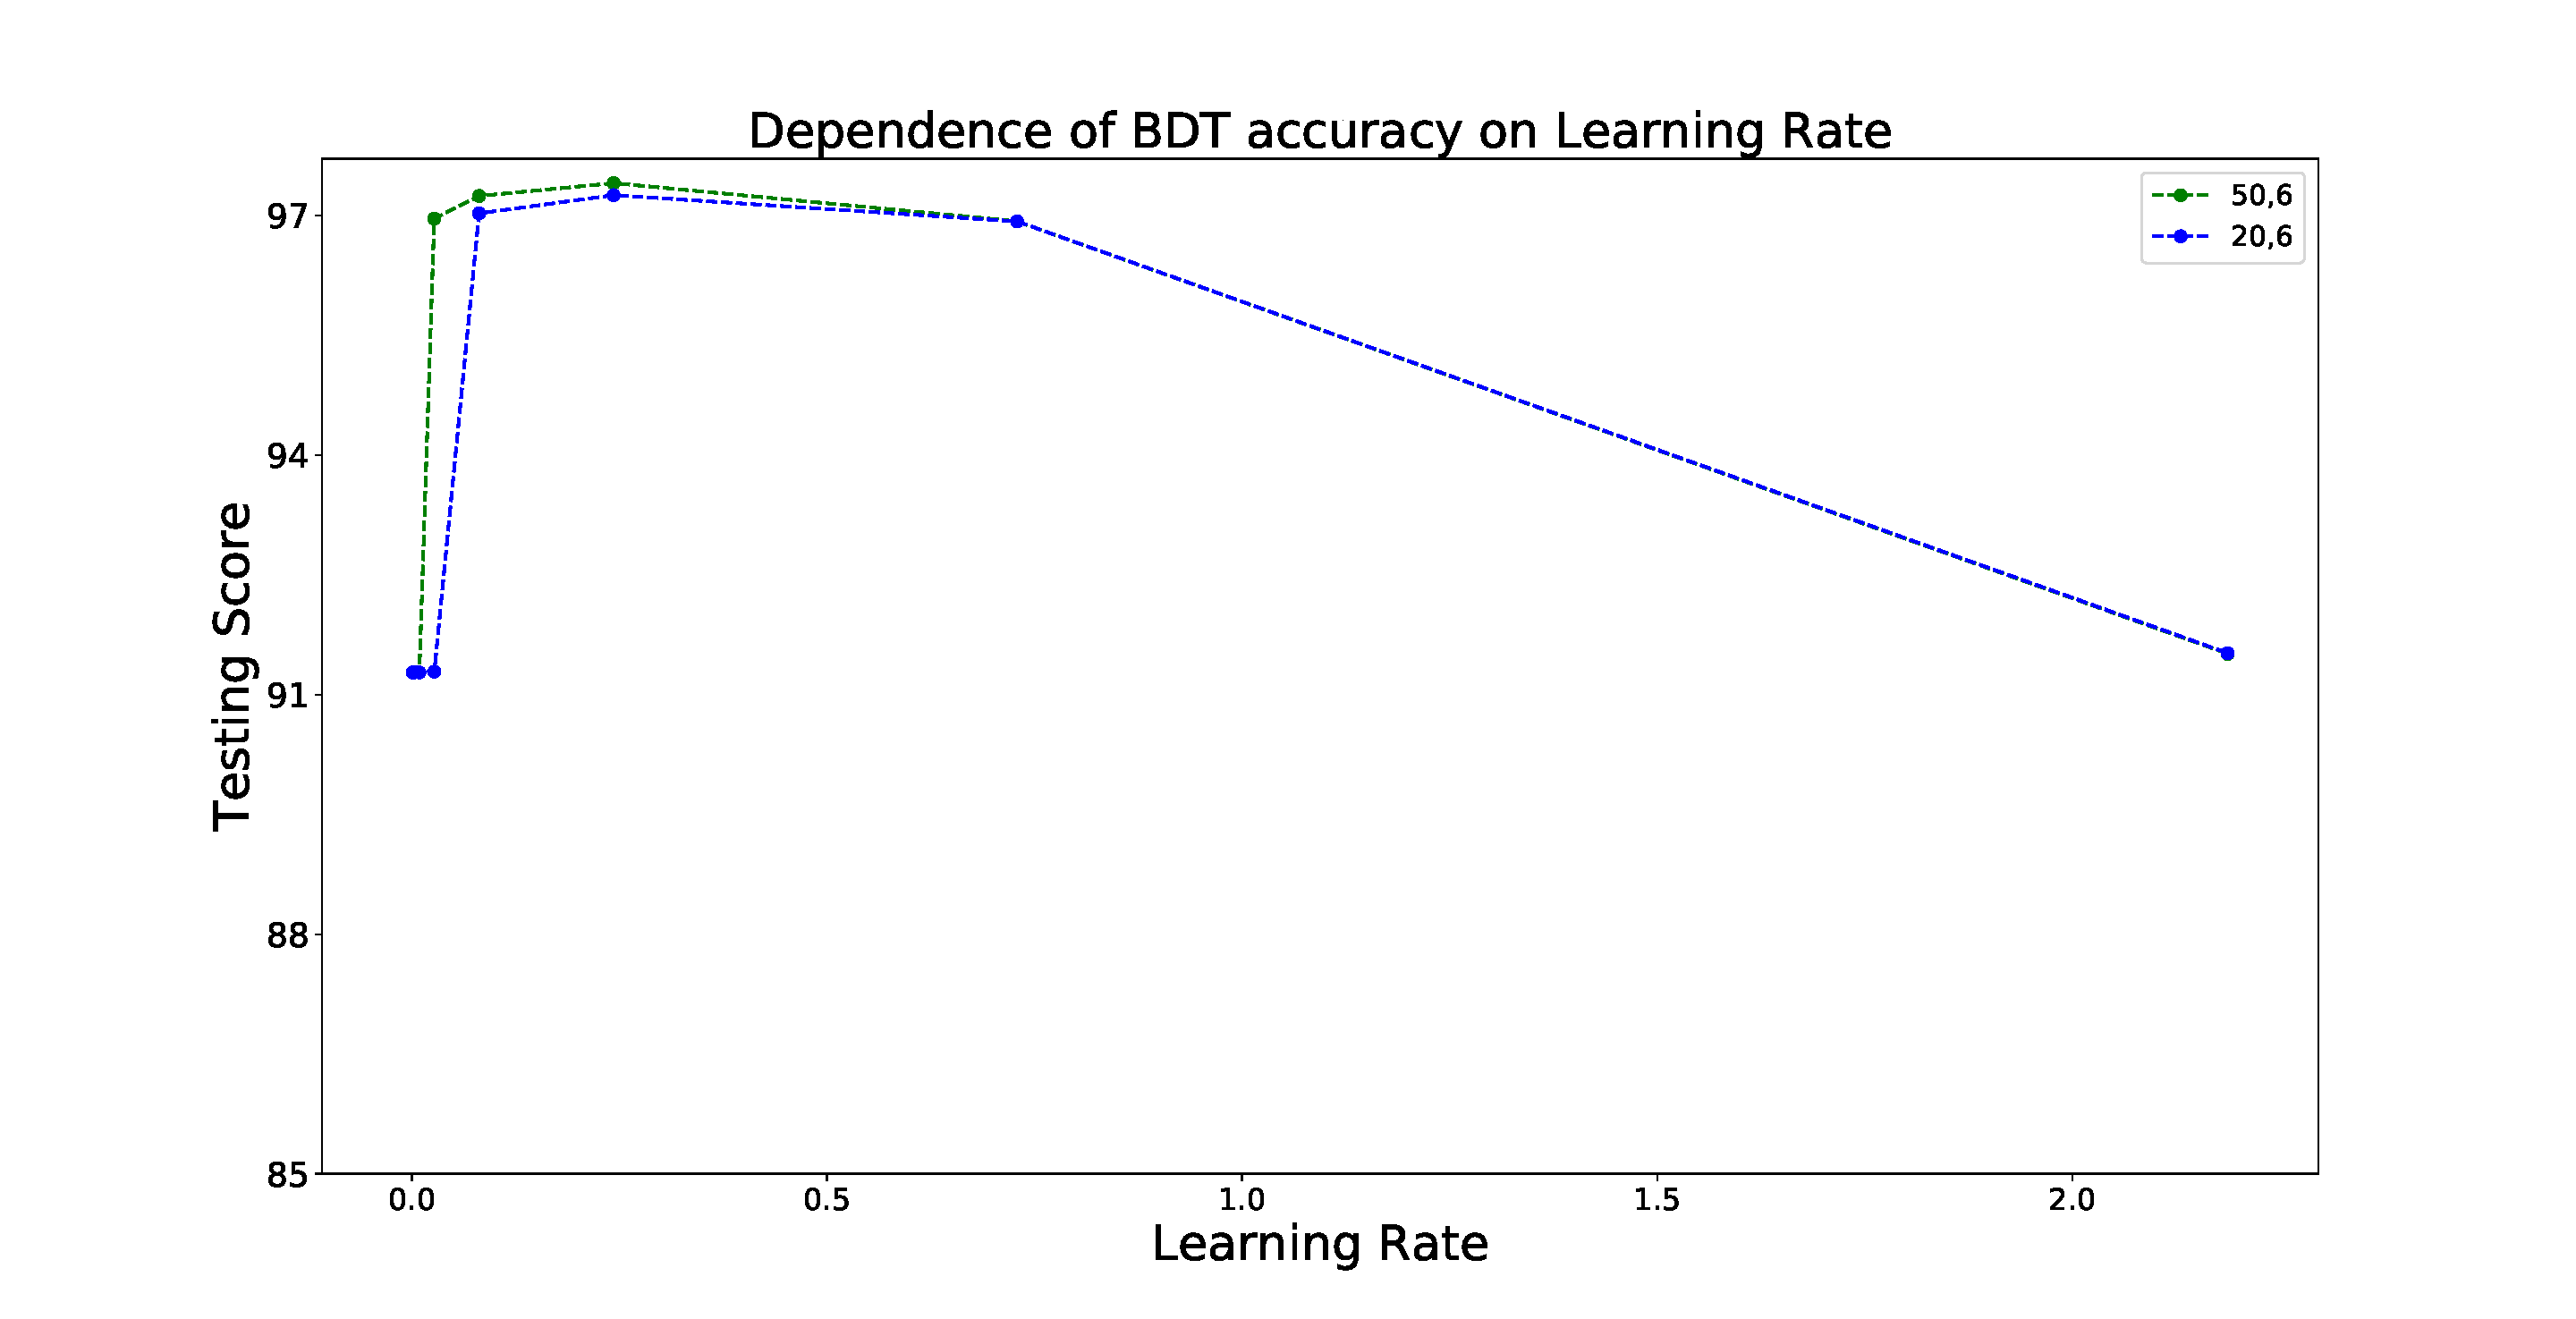
\includegraphics[width=\twopicsp\textwidth]{plots/lr.pdf}
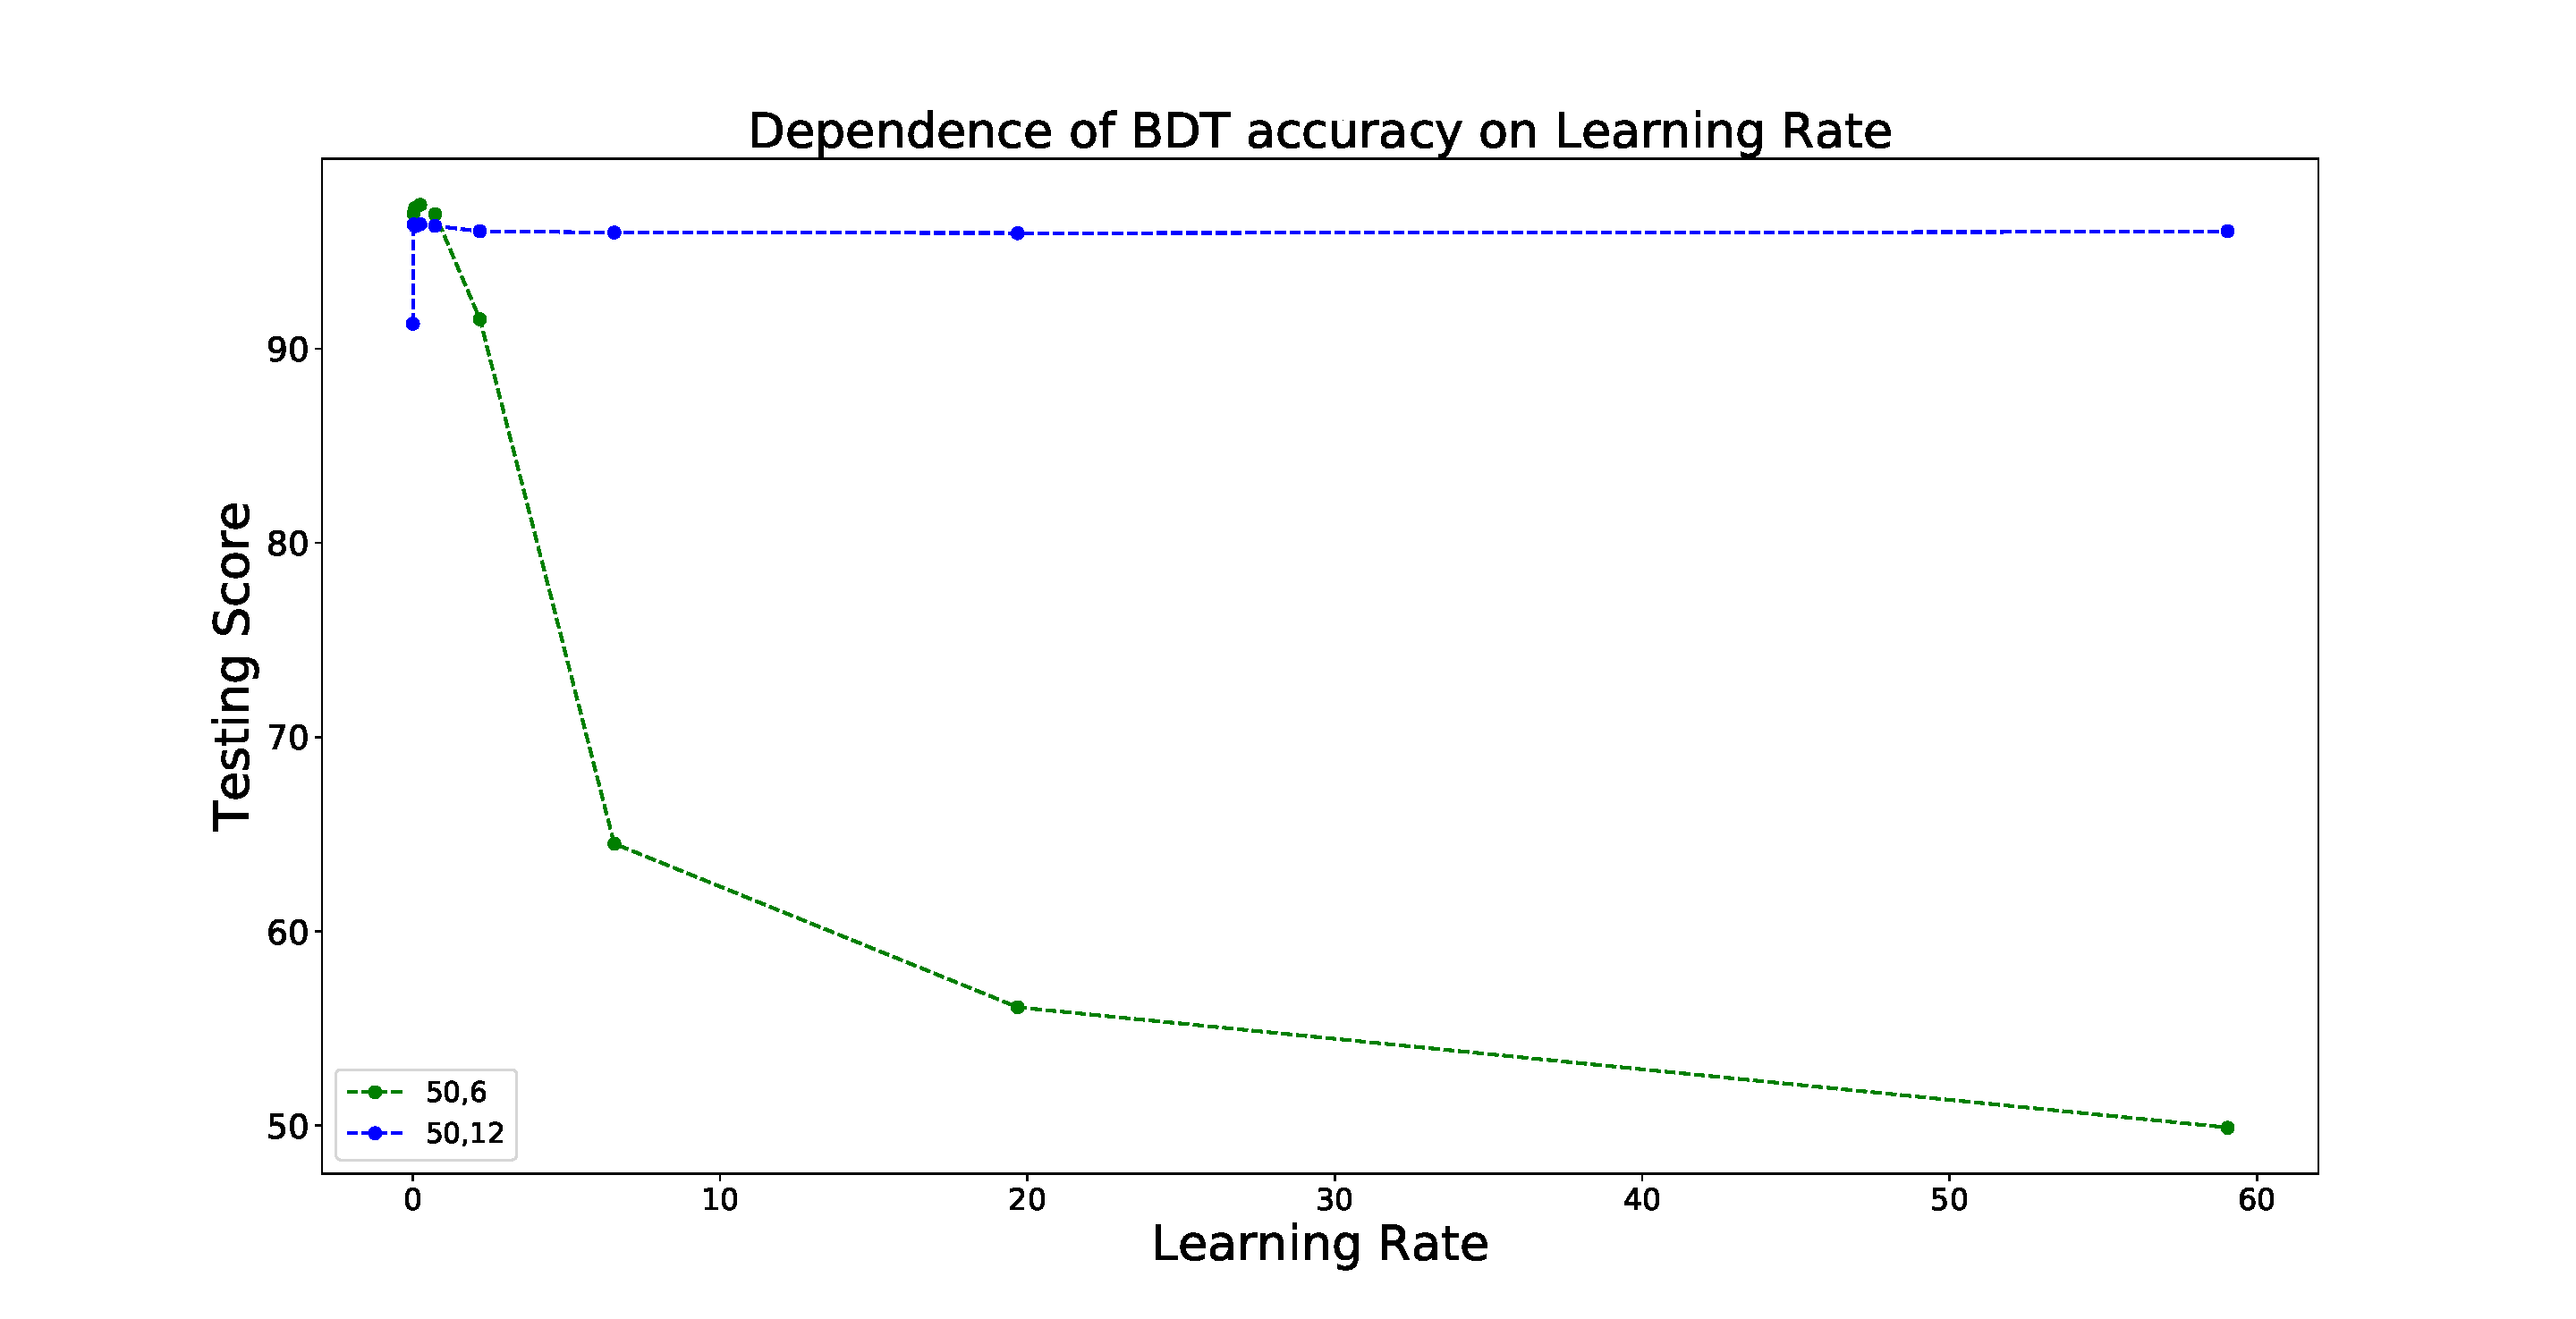
\includegraphics[width=\twopicsp\textwidth]{plots/lr3.pdf}
\caption{Dependence of BDT accuracy on learning rate with number of trees and maximum depth kept constant.
\dima{I'd include the name of the algorithm in the filenames, so that we can easier find them in the folder. ``lr'' sounds more like logistic regression.}}
\label{fig:BDT_learning_rate}
\end{figure}
\end{comment}




\subsection{Logistic Regression}

Logisitc Regression parameters include maximum iterations, tolerance, and a regularization parameter. In the figure below on can see that iterations change the accuracy only for the saga solver, and both lbfgs and liblinear are unchanged. The latter are faster algorithms good for smaller datasets like ours. Furthermore for our data set there is no strict dependence on the tolerance and after a threshold vale the regularization also produces the same result.
%\dima{Which parameters do we use for the final algorithm? For some set of parameters, the LR should be equivalent to NN in our case,
%in particular, the domains should be exactly the same (up to numerical convergence). 
%We can discuss several solvers, but for plots and further calculations I'd suggest to choose one solver and use only it, 
%I'm not sure if many people would be interested to see a dependence on the solver.}


\begin{figure}[h]
%\centerin
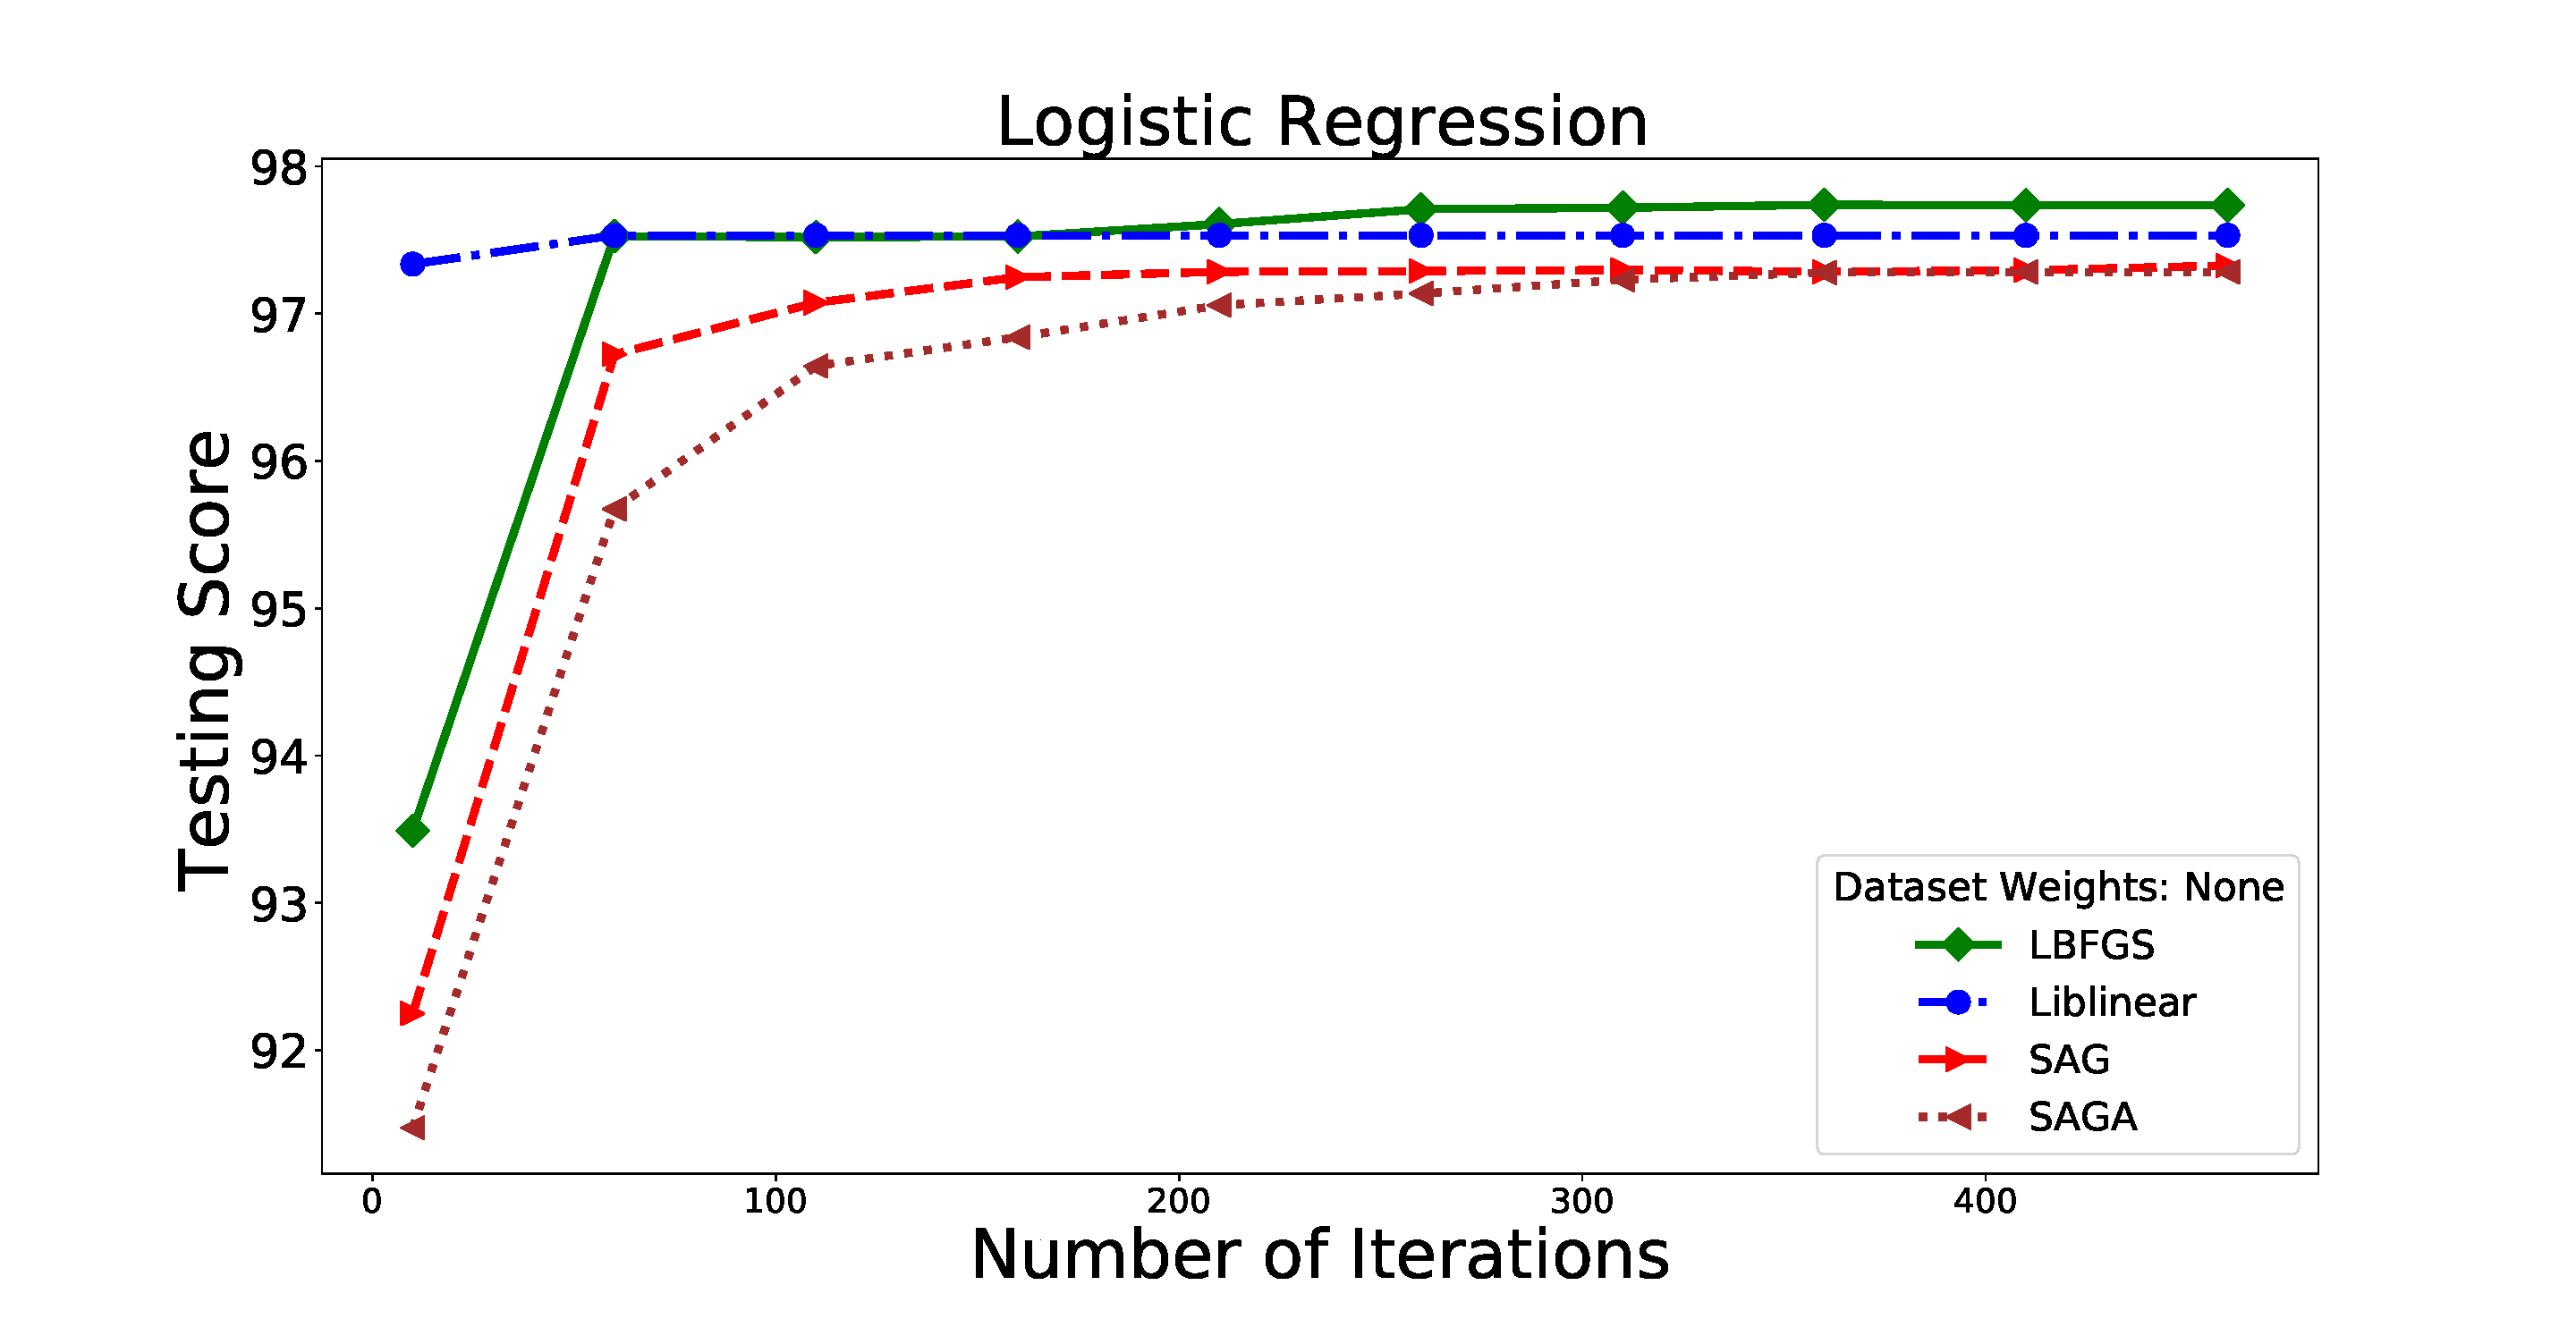
\includegraphics[width=\twopicsp\textwidth]{plots/lr_train.pdf}
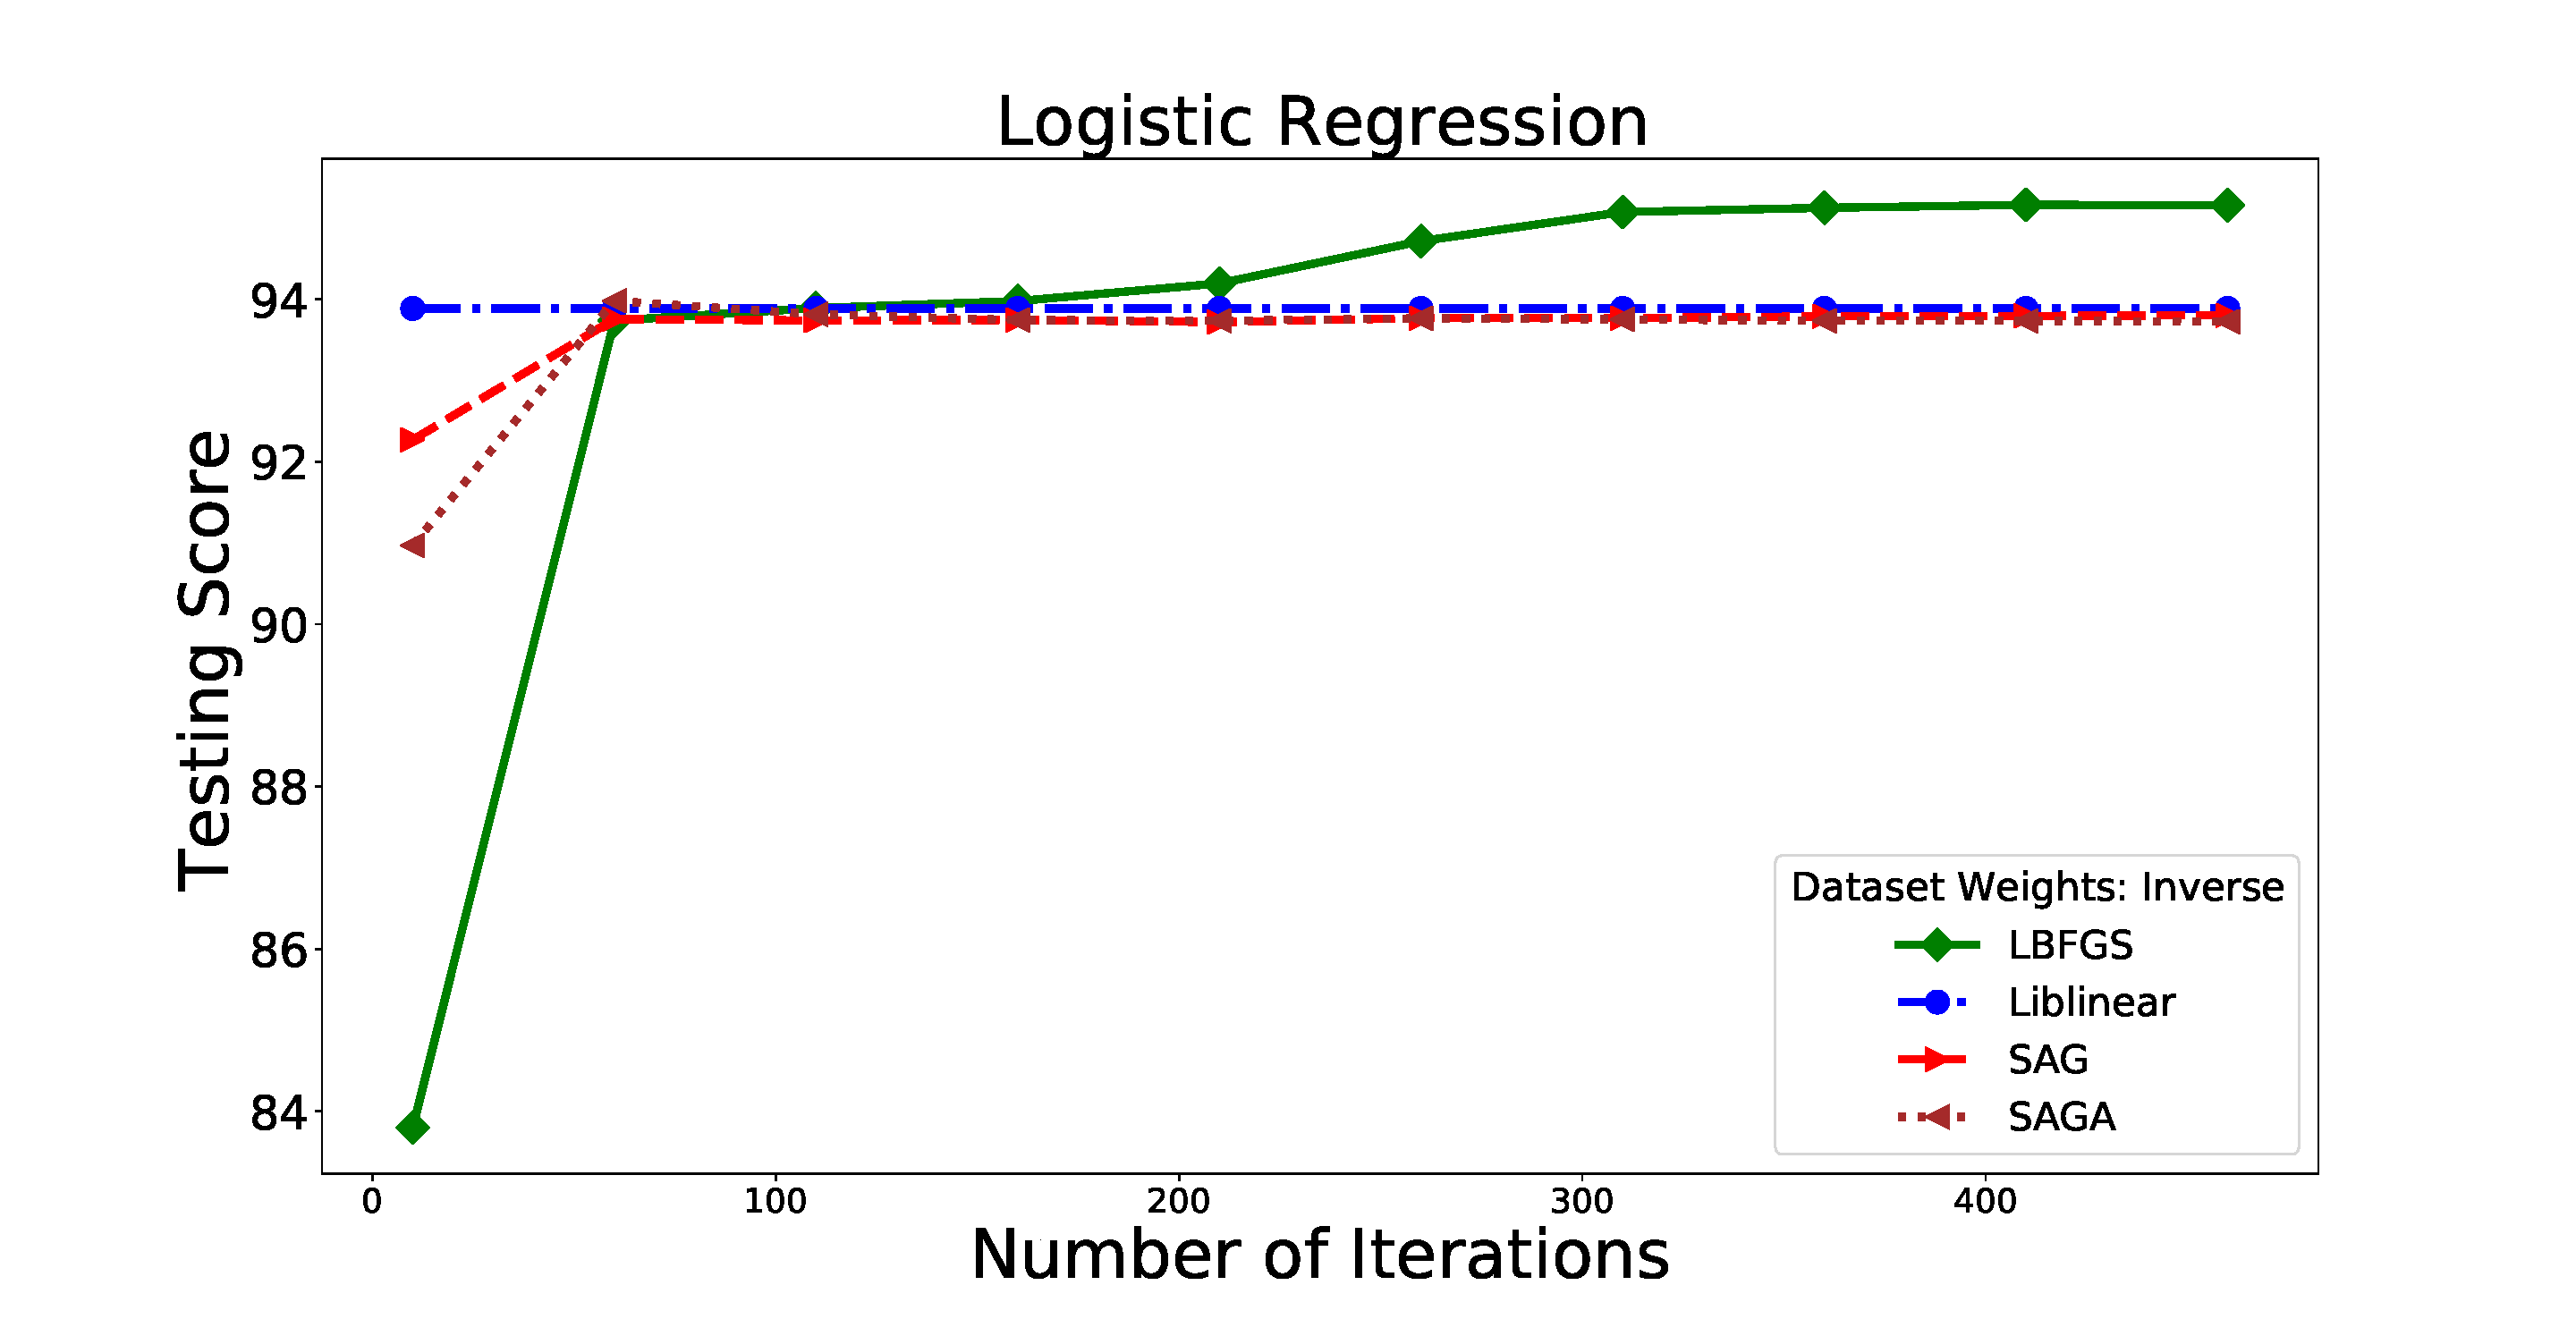
\includegraphics[width=\twopicsp\textwidth]{plots/lr_train_weights.pdf}
\caption{Dependence of LR accuracy on Iterations for different solvers. The difference in accuracy due to weighting is almost 3\% and therefore a significnt effect.}
%\dima{I think it's a wrong plot for regularization (it says tolerance in the plot title). 
%I'm not sure we need to plot accuracy vs tolerance or iterations.
%Also please add the algorithm names in the filenames.}}
\label{fig:LR_accuracy}
\end{figure}

Classification domains are presented in Figure \ref{fig:LR_domains}. As can be seen, when a Neural Network with no hidden layer is compared, the results are almost identical. \\

\begin{figure}[h]
%\centerin
\hspace*{-1.5cm}
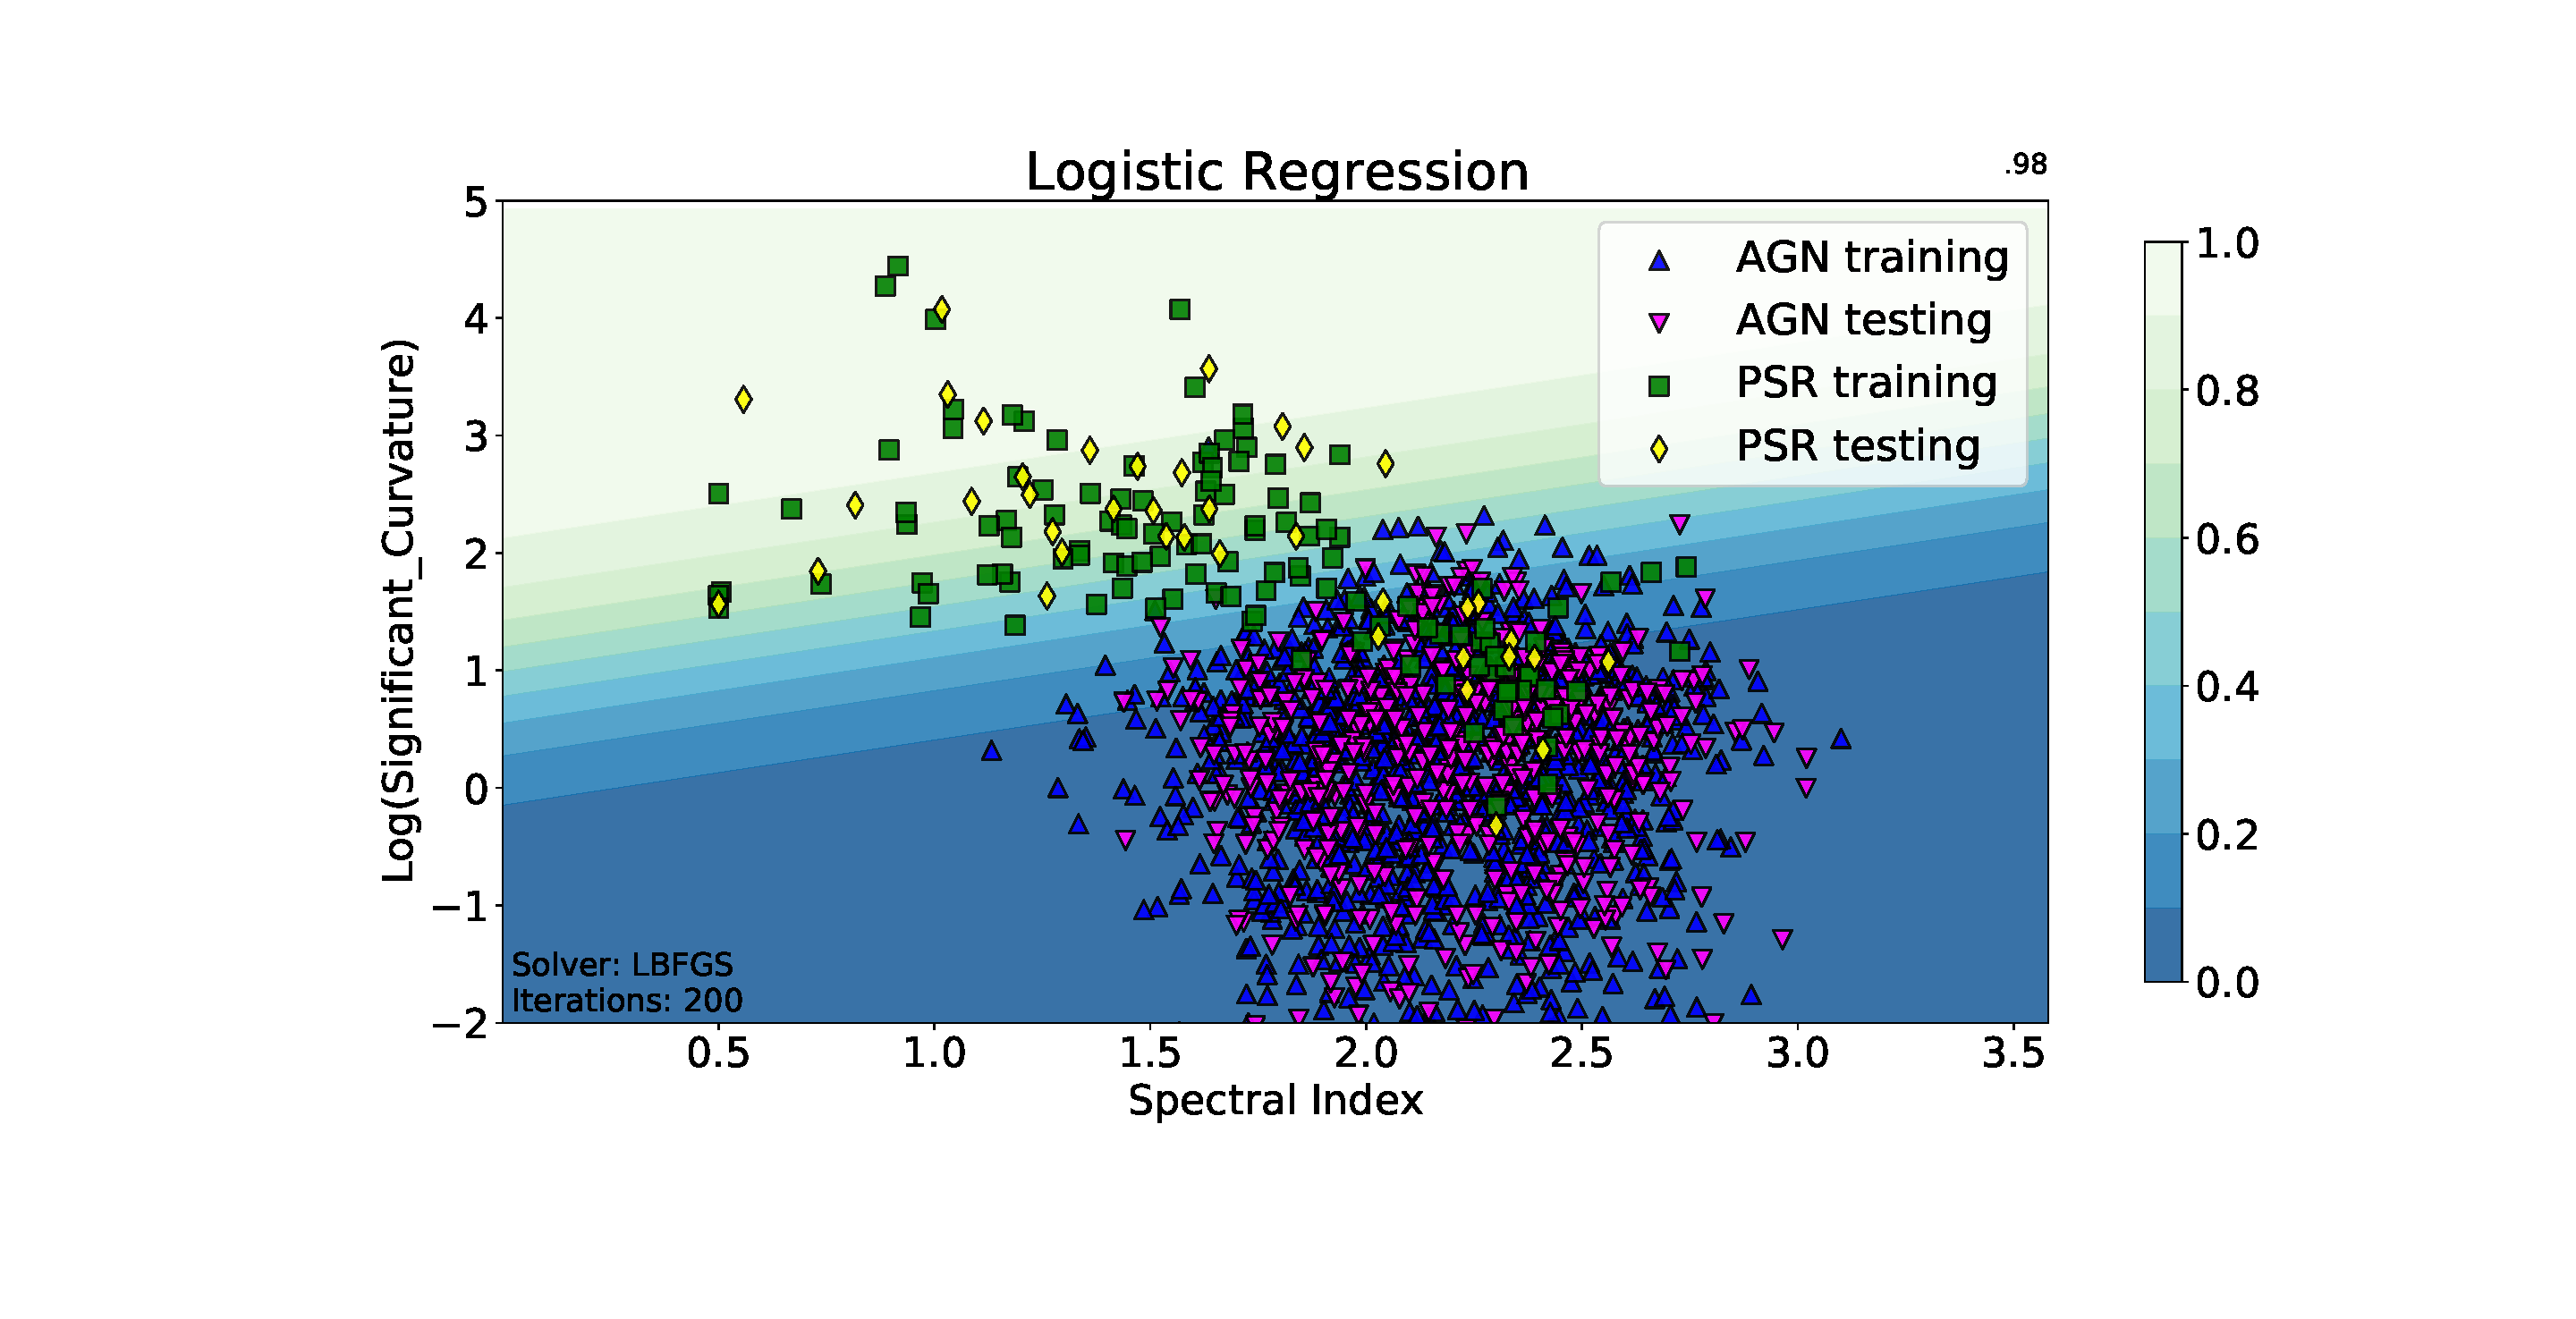
\includegraphics[width=0.6\textwidth]{plots/classification_domains/lr_200_lbfgs.pdf}
%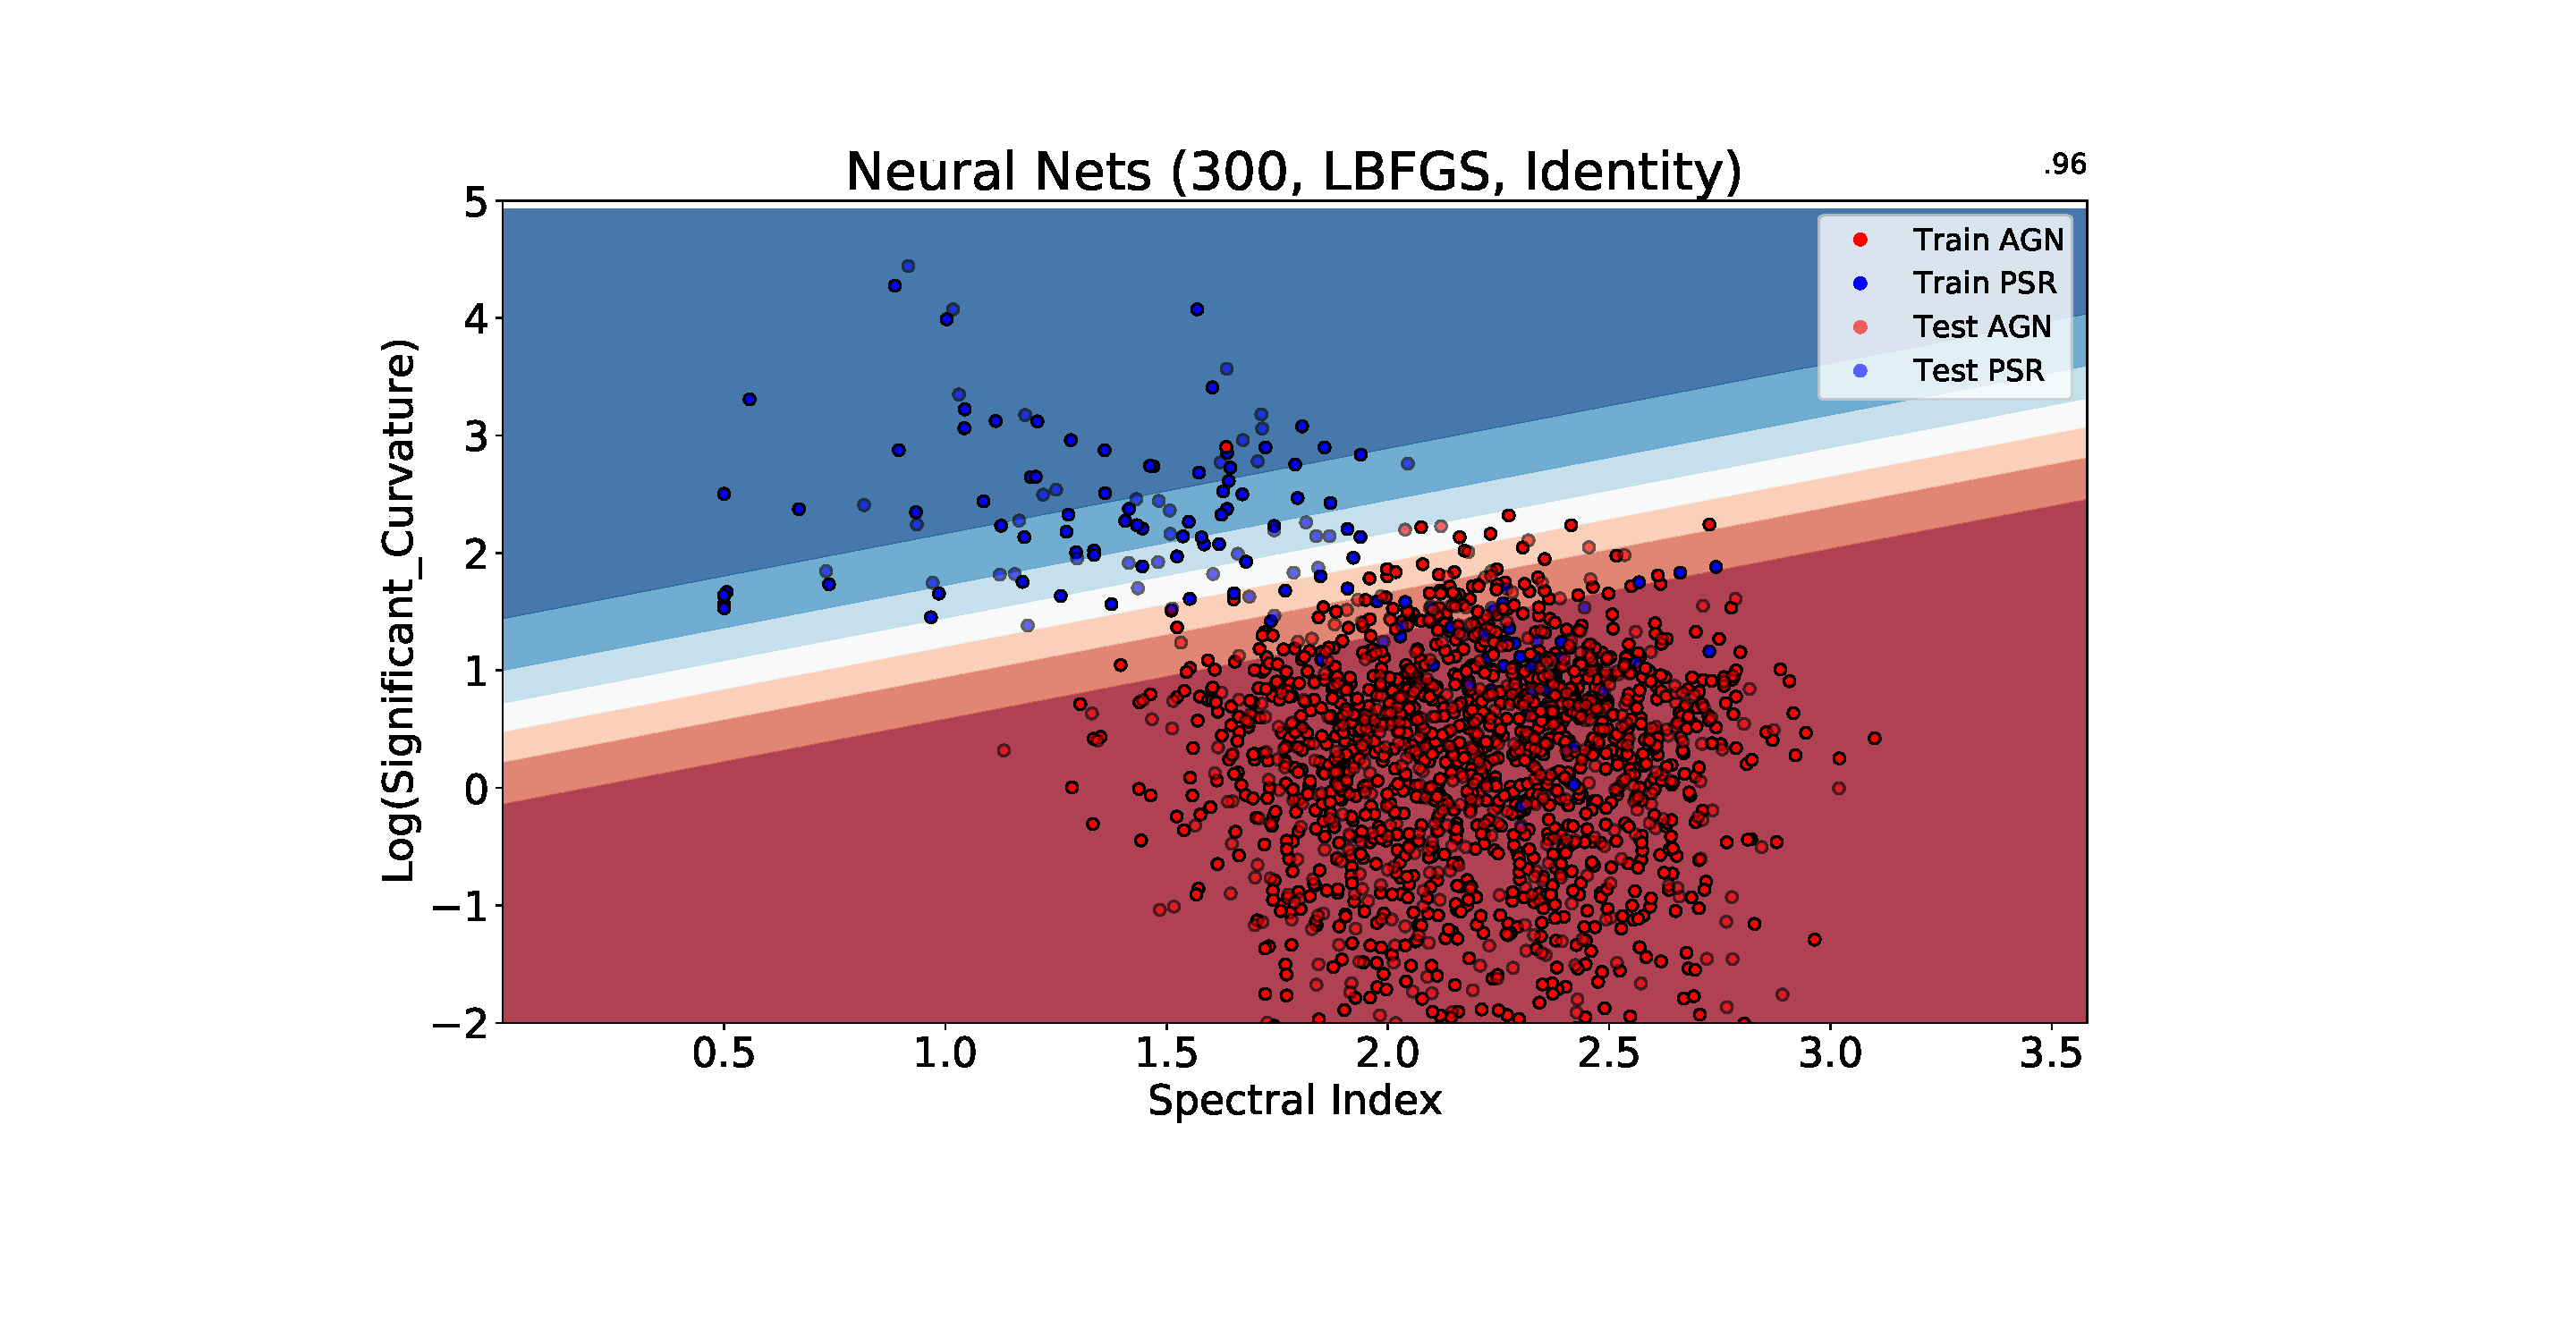
\includegraphics[width=\twopicsp\textwidth]{plots/classification_domains/NN_300_LBFGS_Identity.pdf}
\caption{Classification domains for Logistic Regression}
%\dima{There should be a set of parameters, which gives the same result as for the NN in Figure \ref{fig:NN_domains}.}}
\label{fig:LR_domains}
\end{figure}


